% !TeX program = pdflatex
% !TeX root = main.tex
\documentclass[twoside,twocolumn,9pt]{article}
\usepackage{extsizes}
\usepackage[super,sort&compress,comma]{natbib}
\usepackage[left=1.5cm,right=1.5cm,top=1.785cm,bottom=2.0cm]{geometry}
\usepackage{amsmath,amssymb,amsfonts,amsthm}
\usepackage{array,tabularx,booktabs}
\usepackage{graphicx,float,placeins}
\usepackage{balance,lastpage,fancyhdr,fnpos}
\usepackage[format=plain,justification=justified,singlelinecheck=false,font={stretch=1.125,small,sf},labelfont=bf,labelsep=space]{caption}
\usepackage[english]{babel}
\usepackage{mathptmx,sectsty,droidsans,charter}
\usepackage[T1]{fontenc}
\usepackage[usenames,dvipsnames]{xcolor}
\usepackage{setspace}
\usepackage[compact]{titlesec}
\usepackage{url}
\usepackage{hyperref}
\hypersetup{
  hidelinks,
  pdftitle={Increasing electricity exports through delivery-informed allocation in distribution networks},
  pdfauthor={Junjie Huang, Tao Yu, Zhenning Pan, Yufeng Wu, Wencong Xiao, Rankai Zhu, Jie Huang, and Yusheng Xue}
}
\usepackage{epstopdf}

\addto{\captionsenglish}{\renewcommand{\refname}{Notes and references}}
\definecolor{cream}{RGB}{222,217,201}
\definecolor{rscbar}{RGB}{151,171,190}
\newtheorem{assumption}{Assumption}
\newtheorem{proposition}{Proposition}[section]
\newtheorem{definition}{Definition}[section]
\newtheorem{theorem}{Theorem}[section]
\newcommand{\suppref}{\textit{Supporting Information}\textsuperscript{\dag}}
% Real repository; author-review access status is stated in Data availability.
\newcommand{\repositoryurl}{\url{https://github.com/MarxHuang/ecf-export-access}}

\begin{document}
\raggedbottom
\pagestyle{fancy}
\thispagestyle{plain}
\fancypagestyle{plain}{\renewcommand{\headrulewidth}{0pt}}
\makeFNbottom
\makeatletter
\renewcommand\LARGE{\@setfontsize\LARGE{15pt}{17}}
\renewcommand\Large{\@setfontsize\Large{12pt}{14}}
\renewcommand\large{\@setfontsize\large{10pt}{12}}
\renewcommand\footnotesize{\@setfontsize\footnotesize{7pt}{10}}
\renewcommand\@biblabel[1]{#1}
\renewcommand\@makefntext[1]{\noindent\makebox[0pt][r]{\@thefnmark\,}#1}
\makeatother
\renewcommand{\thefootnote}{\fnsymbol{footnote}}
\renewcommand\footnoterule{\vspace*{1pt}\color{cream}\hrule width 3.5in height 0.4pt\color{black}\vspace*{5pt}}
\renewcommand{\figurename}{\small Fig.~}
\sectionfont{\sffamily\Large}
\subsectionfont{\normalsize}
\subsubsectionfont{\bfseries}
\setstretch{1.125}
\setlength{\skip\footins}{0.8cm}
\setlength{\footnotesep}{0.25cm}
\setlength{\jot}{7pt}
\titlespacing*{\section}{0pt}{4pt}{4pt}
\titlespacing*{\subsection}{0pt}{12pt}{1pt}
\setlength{\columnsep}{6.5mm}
\setlength{\bibsep}{0.9pt}
\setlength{\textfloatsep}{7pt plus 2pt minus 2pt}
\setlength{\floatsep}{6pt plus 2pt minus 2pt}
\setlength{\intextsep}{6pt plus 2pt minus 2pt}
\renewcommand{\topfraction}{0.92}
\renewcommand{\textfraction}{0.06}
\fancyfoot{}
\fancyfoot[LO,RE]{\vspace{-7.1pt}
\includegraphics[height=9pt]{head_foot/LF}}
\fancyfoot[CO]{\vspace{-7.1pt}\hspace{13.2cm}
\includegraphics{head_foot/RF}}
\fancyfoot[CE]{\vspace{-7.2pt}\hspace{-14.2cm}
\includegraphics{head_foot/RF}}
\fancyfoot[RO]{\footnotesize\sffamily 1--\pageref{LastPage}~\textbar\hspace{2pt}\thepage}
\fancyfoot[LE]{\footnotesize\sffamily \thepage~\textbar\hspace{3.45cm}1--\pageref{LastPage}}
\fancyhead{}
\renewcommand{\headrulewidth}{0pt}
\renewcommand{\footrulewidth}{0pt}

\twocolumn[
\begin{@twocolumnfalse}
 {{\sffamily\bfseries\Large Energy \& Environmental Science}\hfill
 \raisebox{0pt}[0pt][0pt]{
\includegraphics[height=55pt]{head_foot/RSC_LOGO_CMYK}}\\[1ex]
{\setlength{\fboxsep}{0pt}\colorbox{rscbar}{\parbox[c][1.28cm][c]{18.5cm}{\hspace{0.55cm}\color{white}\sffamily\bfseries\large PAPER}}}}\par
\vspace{1em}
\sffamily
\begin{tabular}{@{}m{4.2cm}@{\hspace{0.25cm}}p{13.3cm}@{}}

\includegraphics{head_foot/DOI} & \noindent\raggedright\arraybackslash\LARGE\textbf{Increasing electricity exports through delivery-informed allocation in distribution networks$^\dag$} \\
\vspace{0.3cm} & \vspace{0.3cm} \\
& \noindent\large Junjie Huang,\textit{$^{a}$} Tao Yu,\textit{$^{a}$} Zhenning Pan,\textit{$^{a}$} Yufeng Wu,\textit{$^{a}$} Wencong Xiao,\textit{$^{a}$} Rankai~Zhu,\textit{$^{a}$} Jie~Huang,\textit{$^{b}$} and Yusheng Xue\textit{$^{\ast c}$} \\

\includegraphics{head_foot/dates} & \noindent\normalsize
 When distribution networks are constrained, how export access is shared
 affects how much locally generated electricity reaches the grid. In
 request-based allocation, access is assigned before participants know how
 much they can export. Unused export permission can block delivery elsewhere,
 but a shortfall alone cannot establish that loss. Automatically tightening
 future access can also prevent useful delivery when output recovers. We model
 how participants choose requests before their available output is known. The analysis identifies
 when a larger request improves the participant's expected payoff but reduces
 total delivery. We propose externality-conditioned counterfactual feedback
 (ECF) to update future request ceilings using completed operating records.
 After each interval, ECF recalculates the allocation for that interval,
 capping requests from participants with unused awards at their completed
 delivery. The calculation retains the interval's loads, network topology, limits and
 allocation rule. It uses post-event estimates of available export to
 calculate what each participant could have delivered. Future ceilings tighten
 for the unused-award group only if the alternative releases access for
 others, increases their delivery and total delivery, and passes
 alternating-current (AC) power-flow checks. Otherwise, ceilings recover toward
 registered capacity. Controlled medium-voltage simulations test five
 allocation rules. With a moderate update weight and no shortfall charge, ECF
 delivers more electricity on average than spreading the same total request
 reduction proportionally across participants. In a separate 80-day Australian
 simulation using public photovoltaic and load profiles, ECF increases modeled
 delivery by 0.59\% relative to either no feedback or this equal-total control.
 Total authorization rises while its unused portion falls relative to no
 feedback. A control that applies the same ceiling update after every unused
 award leaves less permission unused than ECF, yet ECF delivers 2.76\% more
 electricity. Giving the latest interval full weight instead
 reduces total delivery below the no-feedback level. These findings distinguish
 increasing delivered electricity from merely reducing unused permission.
 They show how completed operating records can improve future export allocation
 without changing network limits or replacing the allocation rule. \\
\end{tabular}
\end{@twocolumnfalse}\vspace{0.2cm}
]

\renewcommand*\rmdefault{bch}\normalfont\upshape
\rmfamily
\section*{}
\vspace{-1cm}
\footnotetext{\textit{$^{a}$ School of Electrical Engineering, South China University of Technology, and Guangdong Provincial Key Laboratory of Intelligent Measurement and Advanced Metering of Power Grid, Guangzhou 510640, China. E-mail: ep0129rkzhu@mail.scut.edu.cn (Rankai Zhu).}}
\footnotetext{\textit{$^{b}$ NARI Technology Co., Ltd., Nanjing 211106, China.}}
\footnotetext{\textit{$^{c}$ State Grid Electric Power Research Institute (NARI Group Corporation), Nanjing 211106, China. E-mail: xueyusheng@sgepri.sgcc.com.cn.}}
\footnotetext{\dag~Supporting Information (SI), code, calculated results, and figure data are deposited at \repositoryurl. Access is currently restricted to author review; see Data availability.}

\section*{Broader context}
The growth of distributed generation makes better use of existing network
capacity important alongside network expansion. Flexible export arrangements
in South Australia, California, and the EU manage generation within network
limits \cite{sapn2024dapr,cpuc2022e5230,eu2024flexibleconnections}; China's
distributed photovoltaic requirements also emphasize connection capacity and
controllability \cite{nea2025distributedpv}. These developments make access to
constrained networks an ongoing operating concern. Yet permission to export
and electricity delivered are different outcomes. Where participants request
access before output is known, an unused award can prevent another connection
from supplying electricity that was available. Reducing requests after every
shortfall is not enough: it can also remove access needed when output recovers.
The challenge is to learn from unused awards without treating all of them as
lost opportunities. This study uses completed operating records to identify
when an alternative allocation could have delivered more electricity, then
uses that comparison to guide later requests. Existing network limits,
allocation rules, and settlement arrangements remain in place. The resulting
operating principle is to judge an adjustment by the delivery it enables,
not simply by the unused permission it removes. It requires a reliable record
of available export, because metered shortfall alone cannot show what others
could have delivered.

\section{Introduction}
\label{sec:introduction}
\subsection{Background and Motivation}

Distributed generation, including photovoltaic (PV) generation, can supply the
wider power system only if local networks can carry the electricity not
consumed on-site. Voltage and equipment-loading limits constrain simultaneous
export at some locations and times. Operating envelopes translate these
constraints into connection-level bounds
\cite{petrou2021dynamiclimits,liu2022opfenvelopes,hoque2024doemarket}, which
increasingly form part of flexible export and connection arrangements
\cite{sapn2024dapr,cpuc2022e5230,eu2024flexibleconnections,nea2025distributedpv}.
When several connections share a binding limit, assigning access to one can
restrict another. How access is shared then affects not only permission to
export, but also how much available electricity reaches the network.

Request-based allocation introduces a timing problem. Participants ask for
access before their available export is fully known, and the allocation rule
divides access using those requests. A large request protects delivery if
output is high, but can leave part of the resulting award unused if output is
low. Such a request can reflect uncertainty, private information, or a rational
preference to preserve access for a high-output outcome
\cite{mallaki2021strategic,ellman2021baseline,wang2022baseline}. Its value to
the participant need not coincide with its effect on other connections.

Fig.~\ref{fig:problem_motivation} shows why an unused award alone cannot reveal
lost delivery. Two connections share a binding network constraint. In (a), both
use their awards fully. In (b) and (c), connection B leaves the same portion
unused, but the consequences differ. Giving A more access would not increase
delivery in (b), because A has no additional electricity available. In (c), A
could use that access, so an alternative allocation under the same conditions
would allow more delivery. An award and its meter reading reveal the shortfall,
but cannot distinguish these two situations.

\begin{figure*}[!t]
\centering
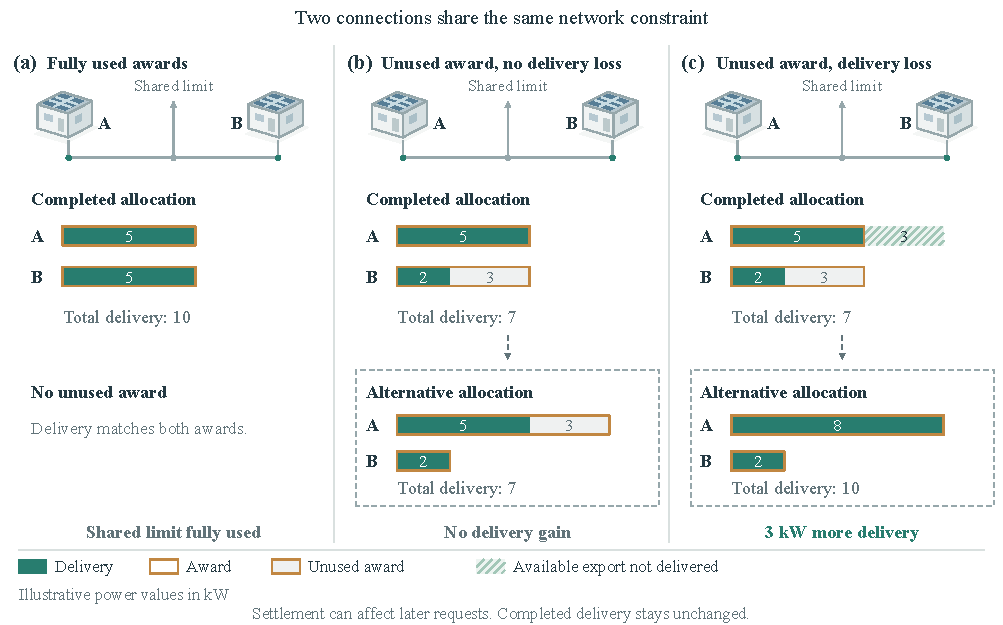
\includegraphics[width=\textwidth]{figures/fig01_problem_motivation.pdf}
\caption{When unused export permission displaces delivery. Two connections
share a binding network constraint. (a) Both awards are fully used.
(b) B leaves part of its award unused, but A has no additional available
export. An alternative allocation increases A's award without increasing
delivery. (c) B leaves the same portion unused while A has available export
that its award prevents it from delivering. The alternative allocation
increases total delivery. Teal fills show delivery, amber outlines show awards,
and hatching shows available export not delivered. Numbers within each segment
give its power in kW. Dashed frames show
calculations for the completed interval. Settlement can affect later requests
but cannot restore that interval's lost delivery. The illustrative values use
a shared 10~kW authorization bound and initial awards of 5~kW each; they are
not case-study results.}
\label{fig:problem_motivation}
\end{figure*}

Neither charging for a shortfall nor reducing all requests answers this
allocation question on its own. A shortfall charge changes the participant's
incentive to request access, whereas the delivery lost elsewhere depends on who
could have used it. Broad reductions can avoid unused awards but also remove
access needed during high-output intervals. The operational challenge is
therefore to use the information revealed after delivery to improve later
allocation, while retaining useful access under uncertainty.

This question extends the closed-loop use of operating information in
cyber--physical power systems \cite{yu2016smartgridcps,xue2017cpsse} to the
sharing of constrained export access. Completed records reveal more than
whether a participant used its award: together with available-export
information, they can show whether a different allocation would have allowed
others to deliver more. The question is how to use that distinction in later
requests without discarding the protection that advance access provides.

\subsection{Related Work}

Operating-envelope research establishes how much export a network can support.
Optimal-power-flow formulations convert voltage and equipment limits into connection
bounds \cite{petrou2021dynamiclimits,liu2022opfenvelopes}. Robust formulations
protect these bounds against uncertain feeder conditions
\cite{liu2022robustdoe,liu2023linearopfdoe}. Regulatory guidance and demonstration
specifications show how flexible limits can be communicated and administered
\cite{aer2024exportlimits,arena2024converge,aemo2023edgedataspec}. Market and
capacity studies incorporate the bounds into secure exchange, bidding, and
capacity assessment
\cite{ullah2021physical,pankhurst2024transactive,hoque2024doemarket,
azim2025doetrading,attarha2022networksecure,mahmoodi2024capacity}.

Within network limits, allocation methods divide access using weighted proportional, equitable, or
bargaining objectives
\cite{petrou2020weighted,alam2023allocation,cuenca2022nonbias,
jiang2025bargaining}. Curtailment studies further show that sharing outcomes
depend on the chosen fairness measure and allocation objective
\cite{liu2020fairness,lusis2020reducing,gupta2024analysis,
gupta2024fairness}. Together, these approaches make export allocation sensitive
to network limits and to the chosen sharing objective. Feasibility, however,
does not ensure that the resulting permission will be used: actual output
becomes known after an award based on requests and forecasts has been issued.

Allocated limits can also be exchanged before delivery. SecuLEx lets customers
trade portions of their operating envelopes before the operating interval,
subject to network-security checks \cite{vassallo2027seculex}. This adjusts
already-issued limits as forecasts or preferences change.

Operating records can also influence subsequent limits. Local-voltage methods
use measurements to calculate operating envelopes
\cite{hashmi2023localvoltage}. Moring et al.\ formulate fairness across multiple
intervals using joint allocation or, in a separate method, allocation
objectives weighted by past curtailment
\cite{moring2024fairovertime}. A recent preprint combines accumulated delivery
ratios, pricing, and constrained matching in a stateful coordination layer
\cite{sweeney2026stateful}. These approaches already connect measured or
historical conditions to allocation. Our question concerns a different use of
the completed record: whether an alternative allocation would have allowed
other participants to deliver electricity that was available at that time.

Participant-choice models explain why those advance requests matter. Local
energy and flexibility-market studies connect network constraints with bids,
prices, payments, and clearing outcomes
\cite{chen2022energy,tsaousoglou2021mechanism,
belgioioso2021operationally}. Game and mechanism models derive participant
choices from incentives rather than treating them as fixed. Demand-response
research shows how reported baselines respond to private incentives, uncertain
events, and later meter data
\cite{ellman2021baseline,wang2022baseline,wang2021selfreported}.
Distribution-level flexibility procurement also represents uncertain resource
availability and unreliable delivery
\cite{tsaousoglou2021uncertainty,essayeh2025stochastic,
mallaki2021strategic,anaya2021flexibility}. These studies connect requests to
incentives and assign consequences to unreliable delivery. They motivate
treating larger requests as choices under uncertainty rather than as arbitrary
reporting errors. They also clarify the distinction needed here: a charge
based on one participant's shortfall and the delivery forgone by other
participants need not have the same magnitude or depend on the same information.

These approaches provide network-feasible allocation, incentives, and several
ways to use operating history. The distinction examined here is not whether
history should matter, but what a completed shortfall justifies changing.
Awards and meter readings identify unused permission. Available-export
information is also needed to determine whether someone else could have used
it. We use that comparison to guide subsequent requests while retaining the
underlying allocation rule.

\subsection{Contributions}

We first identify when protecting a participant's own export reduces total
delivery. A single uncertain-output model generates both request choice and
later delivery, linking the incentive for a larger request to its effect on
other connections. The resulting request--access--delivery externality
distinguishes productive larger requests from those that increase the
requesting group's payoff and unused award while lowering total delivery.
The analysis gives conditions for this divergence and evaluates finite changes
when active network constraints change.

We then introduce externality-conditioned counterfactual feedback (ECF), which
uses recoverable delivery rather than shortfall alone to select later request
updates. It compares the completed allocation with a physically feasible
alternative and tightens future ceilings only when that alternative recovers
delivery elsewhere and increases the total. A bounded update preserves the
existing allocation rule and limits the response to the latest record. The
comparison qualifies an unused-award group; it does not assign individual
responsibility or require private payoff information.

Two matched controls support these contributions. Equal-total reduction
isolates where requests are reduced, while the same update without replay
qualification isolates the value of checking recoverable delivery. Controlled
comparisons connect these effects to request incentives and allocation rules;
public-data simulations examine dynamic response, information quality, and
spatial variation. Section~\ref{sec:concept} explains the operating sequence,
Results develops the findings, and Methods specifies the model. The
\suppref{} supplies the full derivations and supporting analyses.

\long\def\EESsystemmethod{%
\subsection{Network allocation and information timing}
\label{sec:framework}

The model separates three stages: an uncertain request, a network-constrained
award, and delivery limited by realized available export. Feedback carries
information from completed delivery into the next request stage. Let
$\mathcal G=(\mathcal B,\mathcal L)$ denote the distribution-network graph, and
let $\mathcal N$ denote the set of participating connections. The map
$\nu(i)\in\mathcal B$ assigns participant $i$ to a bus.

In interval $t\in\mathcal T$, participant $i$ has a fixed connection bound
$C_i>0$. This bound caps the request admitted to allocation and the resulting
award; the raw request may exceed it. The participant observes a private signal
$s_i(t)$ about its available active-power
export $a_i(t)\ge0$. Its conditional cumulative distribution function (CDF) is
$F_i(\cdot\mid s_i(t))$. The participant submits request $r_i(t)\ge0$ before
availability is realized. The coordinator applies allocation rule $\mathcal R$
under network model $\mathcal M$. It grants export access
$x_i^{\mathcal R,\mathcal M}(t)$. Metered delivery is then
$y_i(t)=\min\{x_i^{\mathcal R,\mathcal M}(t),a_i(t)\}$. We suppress the rule and
model superscripts when they are clear. The request is based on this available-export
model, and delivery is limited by its later realization.

Before allocation, the coordinator does not observe $s_i(t)$, $F_i$, or
$a_i(t)$. Availability is realized during the interval. After completion, the
coordinator observes $y_i(t)$ and receives the specified
available-export record $a_i^{\mathrm{tel}}(t)$. Here, the superscript
$\mathrm{tel}$ denotes the post-event record interface, whether the record is
measured or constructed from specified data. ECF also uses the admitted-request
record, completed allocation, unchanged allocation rule and network model, and
bound $C_i$. The private signal and available-export CDF remain with the
participant.

\begin{assumption}[Post-event available export in the experiments]
\label{ass:post_event_available_export_record}
For each completed controlled interval, the data-generating process records
connection-point available export after allocation and delivery. The controlled
study sets $a_i^{\mathrm{tel}}(t)=a_i(t)$ for every participant. This record is
unavailable when $\mathbf x(t)$ is selected, so it cannot alter that allocation.
The Australian replay instead constructs a profile-derived available-export
proxy from scaled gross-PV and household-consumption profiles. That proxy
generates modeled delivery. The primary replay also uses its unperturbed value
as $a_i^{\mathrm{tel}}(t)$; record sensitivities alter only this replay input.
\end{assumption}

\begin{assumption}[Validity of the same-state replay]
\label{ass:counterfactual_consistency}
After an interval is complete, the replay changes only the admitted request
vector. The network topology $\mathcal G$, exogenous network data $\mathbf z(t)$,
and participant set remain fixed. The allocation rule and its parameters also
remain fixed. The reactive-power setting is part of $\mathbf z(t)$. Available
export remains $a_i(t)$ for the replay. For any replayed access
$\widetilde{\mathbf x}(t)$, delivery is
$\widetilde y_i(t)=\min\{\widetilde x_i(t),a_i(t)\}$. The available-export record must describe
the available export in that completed state. The comparison therefore evaluates two allocations against the same available
export.
\end{assumption}

The second assumption applies when changing the awarded access changes only
connection-point delivery and does not alter the underlying available export in
the completed interval. An inverter, plant controller, or auditable portfolio
process may provide the record. If a different access award would also change
underlying available export through inverter control, storage dispatch,
flexible demand, or portfolio redispatch, the replay must model those responses.
A validated error bound permits the conservative test in
\eqref{eq:robust_replay_lower_bound}. Completed delivery also provides a lower
bound when an available-export record is missing. ECF does not tighten the
later ceiling unless valid records or delivery bounds establish increased
delivery in the replay.

Fig.~\ref{fig:claim_allocation_framework} summarizes this timing in
Section~\ref{sec:concept}. The model below keeps the completed allocation,
post-event replay, and next-interval ceiling as separate objects.

Let $\mathbf r(t)=[r_i(t)]_{i\in\mathcal N}$ and
$\mathbf x^{\mathcal R,\mathcal M}(t)=
[x_i^{\mathcal R,\mathcal M}(t)]_{i\in\mathcal N}$. The vector
$\mathbf r^{\mathrm{cap}}(t)$ is the request after applying bound $C_i$. The
ECF request ceiling is $\psi_i(t)\in[0,C_i]$. It starts at $C_i$ and is
updated in Section~\ref{sec:filtering}. The admitted request vector is
$\mathbf r^{\mathrm{adm}}(t)=[r_i^{\mathrm{adm}}(t)]_{i\in\mathcal N}$:
\begin{equation}
r_i^{\mathrm{cap}}(t)=\min\{r_i(t),C_i\},\qquad
r_i^{\mathrm{adm}}(t)=\min\{r_i^{\mathrm{cap}}(t),\psi_i(t)\}.
\label{eq:request_layers}
\end{equation}
Before feedback, $\psi_i(t)=C_i$, so the two bounded requests coincide. Every
allocation below uses the admitted request, not the unbounded submission.

The vector $\mathbf z(t)$ contains exogenous network inputs. These include
loads, fixed injections, reactive-power assumptions, network limits, and fixed
model coefficients. Voltage, branch flow, and other solved quantities belong to
$\boldsymbol\xi_{\mathrm{net}}$. They are not components of $\mathbf z(t)$. The
network feasible set is
\begin{equation}
\mathcal F_{\mathcal M}(\mathcal G,\mathbf z(t))
=
\left\{(\mathbf x,\boldsymbol\xi_{\mathrm{net}}):
\begin{array}{l}
\mathbf f_{\mathcal M}^{\mathrm{eq}}(\mathbf x,\boldsymbol\xi_{\mathrm{net}};\mathcal G,\mathbf z(t))=\mathbf{0},\\[1mm]
\mathbf f_{\mathcal M}^{\mathrm{ineq}}(\mathbf x,\boldsymbol\xi_{\mathrm{net}};\mathcal G,\mathbf z(t))\le\mathbf{0}
\end{array}
\right\},
\label{eq:network_feasible_set}
\end{equation}
where $\mathbf f_{\mathcal M}^{\mathrm{eq}}$ and
$\mathbf f_{\mathcal M}^{\mathrm{ineq}}$ collect the network equations and
limits. The allocation map is
\begin{equation}
\mathbf x^{\mathcal R,\mathcal M}(t)
=
\Pi_{\mathcal R}\!\left(
\mathbf r^{\mathrm{adm}}(t);\,
\mathcal F_{\mathcal M}(\mathcal G,\mathbf z(t)),
\boldsymbol\eta_{\mathcal R}(t)
\right).
\label{eq:general_allocation_map}
\end{equation}
The vector $\boldsymbol\eta_{\mathcal R}(t)$ contains allocation weights and
other rule or objective parameters. Network equations and limits instead belong
to $\mathcal F_{\mathcal M}$ through $\mathcal G$ and $\mathbf z(t)$.
ECF changes neither: its ceiling changes the admitted-request input when the
ceiling binds. This separation permits the same feedback to be compared under
different allocation rules.

The controlled study computes all five allocations with the AC-derived affine
second-order cone program (SOCP) proxy in
Section~\ref{sec:rules_models}. The closed-form expressions given later for WP,
ER, and EA explain local rule behavior; they do not replace the conic network
model in the experiments. Radial AC power flow verifies every resulting
allocation afterward.

For fixed $\mathcal G$, $\mathbf z(t)$,
$\boldsymbol\eta_{\mathcal R}(t)$, and current ceilings
$\{\psi_i(t)\}_{i\in\mathcal N}$, the local request-to-access Jacobian includes
the capacity and admission layers:
\begin{equation}
\mathbf J_x^{\mathcal R,\mathcal M}(\mathbf r(t);t)
=
\frac{\partial\mathbf x^{\mathcal R,\mathcal M}(t)}
{\partial\mathbf r(t)}.
\label{eq:access_sensitivity}
\end{equation}
For $i\ne j$, a negative off-diagonal entry
$J_{x,ji}^{\mathcal R,\mathcal M}$ has a direct meaning. Participant $j$
receives less access when $r_i$ increases locally. This derivative is valid only within one
smooth regime. If a connection bound, request ceiling, active set, or network
constraint changes, we use paired finite differences.

}

\long\def\EESbehaviormethod{%
\subsection{Request choice and delivery effects elsewhere}

The request model explains why a participant can seek more access even when
that choice reduces delivery elsewhere. Its one-period payoff values own
delivery and charges for unused award. We compare the resulting request with
the forecast-based request before introducing the temporal feedback.

\subsubsection{Request choice under uncertain available export}

Let $a_i^{\mathrm{fcst}}(t)$ be participant $i$'s private point forecast. The
conditional cumulative distribution function
$F_i(\cdot\mid s_i(t))$ describes uncertainty in its available export.

For the payoff derivation, fix the interval, all other requests, the allocation
rule, the network model, the exogenous network data, and the conditional
available-export CDFs. We suppress those fixed arguments below. The reference request
uses the point forecast:
$r_i^{\mathrm{ref}}(t)=a_i^{\mathrm{fcst}}(t)$. For participant $i$, define a
larger request by
\begin{equation}
r_i^{\mathrm{chg}}(\gamma_i)
=\gamma_i r_i^{\mathrm{ref}}(t),
\qquad \gamma_i\ge1.
\label{eq:changed_request}
\end{equation}
All other requests retain their reference values. We then recompute
$\mathbf x(\gamma_i)$ with $t$, $\mathcal G$, $\mathbf z(t)$,
$\boldsymbol\eta_{\mathcal R}(t)$, $\mathcal R$, and $\mathcal M$ fixed. The
scalar $\gamma_i$ is therefore a request multiplier, not a time argument. The
value $\gamma_i=1$ gives the reference side of the matched pair.

Let $\vartheta\ge0$ be the modeled cost per unit of unused award, normalized by
the value per unit of delivered export. The realized payoff proxy, measured in
MW-equivalent units, is
\begin{equation}
u_i(t)=y_i(t)-\vartheta[x_i(t)-y_i(t)]^+.
\label{eq:realized_private_payoff}
\end{equation}
Here $[\,\cdot\,]^+$ is the positive-part operator. For the fixed interval, let
$\bar y_i(\gamma_i)=\mathbb E[\min\{x_i(\gamma_i),a_i\}\mid s_i]$ denote
expected delivery. Let
$\bar h_i(\gamma_i)=\mathbb E[[x_i(\gamma_i)-a_i]^+\mid s_i]$ denote the expected
unused award. Expected total delivery is $\bar Y=\sum_j\bar y_j$. The
participant's expected payoff is
\begin{equation}
\begin{aligned}
U_i(\gamma_i;\vartheta)
&=\bar y_i(\gamma_i)-\vartheta\bar h_i(\gamma_i)\\
&=\mathbb E\!\left[
\min\{x_i(\gamma_i),a_i\}
-\vartheta[x_i(\gamma_i)-a_i]^+
\mid s_i\right].
\end{aligned}
\label{eq:behavioral_payoff}
\end{equation}
The controlled request model selects the smallest payoff-maximizing multiplier
on a fixed grid:
\begin{equation}
\gamma_i^\star
=\min\!\left(
\operatorname*{arg\,max}_{\gamma\in\Gamma}U_i(\gamma;\vartheta)
\right).
\label{eq:endogenous_best_response}
\end{equation}
Here $\Gamma$ is the multiplier grid. Let $q_{\mathrm{pf}}$ denote the
participant reactive-power setting; Q0 and Q95 are specified in
Section~\ref{sec:network_ac}. When the experimental factors are shown
explicitly, we write
$\gamma_i^\star(\vartheta,\sigma,\mathcal R,q_{\mathrm{pf}})$. The uncertainty
scale $\sigma$ enters through the available-export CDF. Both
$q_{\mathrm{pf}}$ and $\mathcal R$ enter through the allocation response.
Participant location and the fixed network model and data remain implicit. For
each multi-interval trajectory, this selected multiplier is held fixed, while
$a_i^{\mathrm{fcst}}(t)$ supplies the time variation. Choosing the smallest
maximizer resolves a payoff tie. The
participant uses its private CDF to make this choice. The coordinator receives
the submitted request and later the completed-state records. Available export
and delivery then obey
\begin{equation}
a_i(t)\sim F_i(\cdot\mid s_i(t)),
\qquad
y_i(t)=\min\{x_i(t),a_i(t)\}.
\label{eq:available_export_delivery_link}
\end{equation}
Equations~\eqref{eq:behavioral_payoff} and
\eqref{eq:available_export_delivery_link} use the same available-export CDF. The
request is chosen under that model, and delivery is a later realization from it.

\subsubsection{Private payoff and effects on aggregate delivery}

The following result separates the participant's incentive from the effect on
aggregate delivery. We suppress the conditional arguments $s_j$.

\begin{proposition}[Marginal effects on private payoff and aggregate delivery]
\label{prop:private_aggregate_request_gradient}
Fix the other requests, exogenous network data, and conditional available-export
CDFs. Suppose
$F_j(\cdot\mid s_j)$ is continuous at $x_j$ and the allocation map is locally
differentiable. Write $J_{ji}=\partial x_j/\partial r_i$ for the corresponding
entry of the request-to-access Jacobian in
\eqref{eq:access_sensitivity}. With
$\bar Y=\sum_j\mathbb E[\min\{x_j,a_j\}\mid s_j]$,
\begin{align}
\frac{\partial U_i}{\partial r_i}
&=J_{ii}\!\left[1-F_i(x_i)-\vartheta F_i(x_i)\right],
\label{eq:private_request_gradient}\\
\frac{\partial\bar Y}{\partial r_i}
&=\sum_{j\in\mathcal N}J_{ji}\left[1-F_j(x_j)\right].
\label{eq:feeder_request_gradient}
\end{align}
\end{proposition}
\noindent\textit{Proof sketch.}
For nonnegative available export,
$\mathbb E[\min\{x,a\}]=\int_0^x[1-F(u)]\,\mathrm du$ and
$\mathbb E[(x-a)^+]=\int_0^xF(u)\,\mathrm du$. Differentiate these two
identities and apply the chain rule through $J_{ji}$. This gives
\eqref{eq:private_request_gradient}--\eqref{eq:feeder_request_gradient}.
Section S2 of the \suppref{} gives the continuous-regime proof. Section S8 treats
request bounds, feedback ceilings, and active-set boundaries. We use derivatives
only within one smooth allocation regime. Otherwise, we use a matched finite
difference.

If $J_{ii}>0$, an interior private optimum targets
$F_i(x_i)=1/(1+\vartheta)$. This choice includes the participant's own delivery
and unused award but omits effects on other participants. Those cross-participant
effects can be negative when requests share a binding constraint, as shown for
the allocation rules in Section~\ref{sec:rule_response}. The normalized
shortfall cost that makes the private marginal payoff equal the marginal change
in aggregate delivery is
\begin{equation}
\vartheta_i^{\mathrm{ext}}
=-\frac{\sum_{j\ne i}J_{ji}[1-F_j(x_j)]}
{J_{ii}F_i(x_i)},
\qquad J_{ii}F_i(x_i)>0.
\label{eq:externality_equivalent_shortfall_cost}
\end{equation}
The value $\vartheta_i^{\mathrm{ext}}$ measures the outside delivery effect per
unit of marginal unused award. It varies with the allocation state and can
change sign. We use it as a local diagnostic.

An allocation response can cross an active-set boundary. The case study
therefore also uses a matched finite-difference counterpart. For one participant's
request step, define
\begin{align*}
\Delta\bar y_i&=\bar y_i^{\mathrm{chg}}-\bar y_i^{\mathrm{ref}},\\
\Delta\bar Y_{\mathcal N\setminus\{i\}}
&=\sum_{j\ne i}(\bar y_j^{\mathrm{chg}}-\bar y_j^{\mathrm{ref}}),\\
\Delta\bar h_i&=\bar h_i^{\mathrm{chg}}-\bar h_i^{\mathrm{ref}}.
\end{align*}
When $\Delta\bar h_i>0$, the corresponding finite-difference cost ratio is
\begin{equation}
\vartheta_{i,\Delta}^{\mathrm{ext}}
=-\frac{\Delta\bar Y_{\mathcal N\setminus\{i\}}}{\Delta\bar h_i}.
\label{eq:finite_difference_externality_equivalent_shortfall_cost}
\end{equation}
We report this ratio only when the unused-award increment is positive. A
positive value then means that the request step reduces delivery outside the
participant. Both
\eqref{eq:externality_equivalent_shortfall_cost} and
\eqref{eq:finite_difference_externality_equivalent_shortfall_cost} quantify a
state-specific delivery effect on other participants.

\subsubsection{Matched classification of request effects}

Let the nonempty set $\mathcal K\subseteq\mathcal N$ contain the participants
whose requests change jointly. Superscripts $\mathrm{ref}$ and $\mathrm{chg}$
denote matched reference and changed-request states. Static cases use the expected
changes
\begin{align}
\Delta U_{\mathcal K}
&=\sum_{i\in\mathcal K}(U_i^{\mathrm{chg}}-U_i^{\mathrm{ref}}),\nonumber\\
\Delta\bar h_{\mathcal K}
&=\sum_{i\in\mathcal K}
(\bar h_i^{\mathrm{chg}}-\bar h_i^{\mathrm{ref}}),
&\Delta\bar Y&=\bar Y^{\mathrm{chg}}-\bar Y^{\mathrm{ref}}.
\label{eq:expected_group_classification_changes}
\end{align}
Dynamic intervals use realized payoff and the change in unused award:
\begin{align}
\Delta u_{\mathcal K}(t)
&=\sum_{i\in\mathcal K}
[u_i^{\mathrm{chg}}(t)-u_i^{\mathrm{ref}}(t)],\nonumber\\
\Delta H_{\mathcal K}(t)
&=\mathop{\sum}_{i\in\mathcal K}\!\left(
[x_i^{\mathrm{chg}}(t)-y_i^{\mathrm{chg}}(t)]^+
-[x_i^{\mathrm{ref}}(t)-y_i^{\mathrm{ref}}(t)]^+\right).
\label{eq:realized_group_classification_changes}
\end{align}
With tolerance $\tau_E$, a static comparison is classified as an externality
when all three components of
$(\Delta U_{\mathcal K},\Delta\bar h_{\mathcal K},-\Delta\bar Y)$ exceed
$\tau_E$. Thus, the changed-request group's combined expected payoff rises, its
combined expected unused award rises, and aggregate delivery falls. A dynamic interval applies the same test to
$(\Delta u_{\mathcal K},\Delta H_{\mathcal K},-\Delta Y)$. A productive high
request case raises combined payoff without a decrease in aggregate delivery
beyond the numerical tolerance. Because $\vartheta\ge0$, the externality
conditions imply that delivery to the changed-request group rises. Aggregate
delivery can then fall only if delivery outside that group falls by more.
Section S2 of the \suppref{} gives the exact bounds. This paired classification
is used for mechanism analysis. The completed-state replay in
Section~\ref{sec:filtering} is the separate operational test that determines
whether a later request ceiling changes.

The controlled experiment evaluates \eqref{eq:endogenous_best_response} on the
forecast-linked probability tree in Section~\ref{sec:case_setup}. This gives a
one-period request and later available-export realization from the same model;
its role is to generate internally consistent controlled cases. Within one
smooth allocation regime, a state-specific shortfall cost could match the local
marginal delivery effect. The required value changes when the state or active
constraints change. ECF instead uses a completed-state replay to decide
whether an unused award warrants a later request-ceiling adjustment.

\subsubsection{Outcome measures}

Every comparison matches the rule, network model, exogenous data, and interval.
Participant-group effects are obtained by summing component changes over the
named group. Static comparisons use the barred quantities defined above. For a
realized matched interval, aggregate metered delivery and unused award are
\begin{align*}
Y^{\mathrm{ref}}&=\sum_i y_i^{\mathrm{ref}}, &
H^{\mathrm{ref}}&=\sum_i[x_i^{\mathrm{ref}}-y_i^{\mathrm{ref}}]^+,\\
Y^{\mathrm{chg}}&=\sum_i y_i^{\mathrm{chg}}, &
H^{\mathrm{chg}}&=\sum_i[x_i^{\mathrm{chg}}-y_i^{\mathrm{chg}}]^+.
\end{align*}
Hence
$\Delta Y=Y^{\mathrm{chg}}-Y^{\mathrm{ref}}$, and delivery loss is
$[-\Delta Y]^+$.

We summarize allocation equality with the capacity-normalized Jain index. Let
$\mathbf C=(C_i)_{i\in\mathcal N}$. All controlled-study connection bounds are
positive, and every reported controlled allocation vector is nonzero. Thus,
\begin{equation}
J_{\mathrm{norm}}(\mathbf x,\mathbf C)
=\frac{(\sum_{i:C_i>0}x_i/C_i)^2}
{|\{i:C_i>0\}|\sum_{i:C_i>0}(x_i/C_i)^2}.
\label{eq:jain_normalized}
\end{equation}
For a matched pair,
$\Delta J_{\mathrm{norm}}=J_{\mathrm{norm}}(\mathbf x^{\mathrm{chg}},\mathbf C)
-J_{\mathrm{norm}}(\mathbf x^{\mathrm{ref}},\mathbf C)$.
The \suppref{} gives the raw Jain index and its boundary conventions.
The externality classification uses the delivery, payoff, and unused-award
changes defined above; the Jain index is reported separately. The classification
therefore differs from ordinary redistribution or forecast error.


}

\long\def\EESallocationmethod{%
\subsection{Allocation rules}
\label{sec:rules_models}

Whether one request changes access elsewhere depends on how the allocation rule
couples participants. The controlled study therefore compares five rules using
the same network data, connection bounds, and conic approximation of the network
limits. Every resulting allocation then undergoes the same radial AC check for
its reactive-power setting. The rules differ in how they select an allocation
within that common domain. WP confines the allocation
to a common proportional ray. ER and EA use one-parameter families defined by a
common reduction and a common cap, respectively. ME and FA optimize directly
over the full conic domain. Within each matched comparison, the rule and its
formulation are held fixed. The operator $\Pi_{\mathcal R}$ maps admitted
requests to authorized access. For an optimization-based rule,
$W_{\mathcal R}$ defines the objective, and $\mathcal F_{\mathcal M}$ supplies
the network constraints.

Table~\ref{tab:policy_taxonomy} lists the rules. Weighted proportional, equal
reduction, equal access, maximum export, and fairness-aware allocation are
abbreviated WP, ER, EA, ME, and FA. The label ME refers here to maximizing
authorized access, not metered delivery. Network
representation is a separate choice:
all five controlled rules use the conic proxy domain for allocation and the same
radial AC procedure for subsequent verification.

\begin{table}[!t]
\caption{Export-access allocation rules used in the controlled study}
\label{tab:policy_taxonomy}
\centering
\footnotesize
\setlength{\tabcolsep}{1.8pt}
\renewcommand{\arraystretch}{1.06}
\begin{tabular}{@{}>{\raggedright\arraybackslash}p{0.38in}>{\raggedright\arraybackslash}p{0.84in}>{\raggedright\arraybackslash}p{0.84in}>{\raggedright\arraybackslash}p{0.91in}@{}}
\hline
Rule & Allocation principle & How requests interact & Experimental role \\
\hline
WP & Common proportional scale \cite{alam2023allocation} & Shared scale and binding proxy constraints & One-parameter scaling benchmark \\
ER & Common absolute reduction \cite{liu2020fairness,lusis2020reducing} & Shared reduction level & One-parameter reduction benchmark \\
EA & Common access cap \cite{alam2023allocation} & Shared cap and capped set & One-parameter cap benchmark \\
ME & Maximum total authorized access \cite{liu2022opfenvelopes,mahmoodi2024capacity} & Request bounds and active proxy constraints & Total-access conic rule \\
FA & Authorized access with a normalized equality term \cite{liu2020fairness,gupta2024analysis,gupta2024fairness} & Request bounds, proxy constraints, and equality term & Access--equality comparison \\
\hline
\end{tabular}
\end{table}

\subsubsection{One-parameter allocation rules}

Each rule uses the admitted requests in \eqref{eq:request_layers}. WP sets
$x_i=\rho r_i^{\mathrm{adm}}$ and chooses the largest feasible common scale
$\rho\in[0,1]$. ER sets $x_i=\max\{0,r_i^{\mathrm{adm}}-\lambda\}$ and chooses the
smallest feasible common reduction
$\lambda\in[0,\max_i r_i^{\mathrm{adm}}]$. EA sets
$x_i=\min\{r_i^{\mathrm{adm}},\mu\}$ and chooses the largest feasible common cap
$\mu\in[0,\max_i r_i^{\mathrm{adm}}]$. These one-parameter allocation families
are evaluated against the same conic proxy domain used below; they are not
separate physical network models.
The \suppref{} gives their equations, zero-request boundary cases, and
analytical forms for one aggregate allowance. A request change can alter the binding
voltage or branch constraint or the membership of a piecewise allocation set.
We then re-solve the allocation rather than extend a local formula across that
boundary.

\subsubsection{Full-domain optimization rules}

The following equations describe one fixed interval, so time arguments are
suppressed. ME and FA use the same affine conic approximation of the AC network
limits without a one-parameter restriction on $\mathbf x$. The proxy has three
main parts. A
second-order cone (SOC) constraint bounds the normalized allocation radius. A
cone at each branch end bounds the affine active- and reactive-power prediction.
Affine rows bound bus voltage. The model assumes $C_i>0$ for every participant.
With $\mathbf D_C=\operatorname{diag}((C_i)_{i\in\mathcal N})$, the normalized
radius $\zeta$ satisfies $\|\mathbf D_C^{-1}\mathbf x\|_2\le\zeta$. Each branch
cone has a nonnegative affine right-hand side in $\zeta$. The \suppref{} gives
the full constraint form and guard-margin definitions. The archived
machine-readable records contain the numerical coefficient arrays.

ME Stage~1 is therefore an SOCP. ME Stage~2 and FA contain
convex quadratic terms. Introducing epigraph variables for those terms gives
equivalent rotated SOC representations. This proxy differs from the branch-flow
relaxation in \cite{farivar2013branch1}. Radial AC power flow supplies the
physical check. The common primary optimization form is
\begin{equation}
\begin{aligned}
\max_{\mathbf x,\boldsymbol\xi_{\mathrm{net}}}\quad
&W_{\mathcal R}(\mathbf x,\mathbf r^{\mathrm{adm}};\boldsymbol\eta_{\mathcal R})\\
\mathrm{s.t.}\quad
&0\le x_i\le r_i^{\mathrm{adm}},\quad i\in\mathcal N,\\
&(\mathbf x,\boldsymbol\xi_{\mathrm{net}})\in
\mathcal F_{\mathcal M}(\mathcal G,\mathbf z).
\end{aligned}
\label{eq:opf_stub}
\end{equation}
Here $\mathbf r^{\mathrm{adm}}$ is the request presented to the optimizer.
The vector $\boldsymbol\xi_{\mathrm{net}}$ contains its endogenous network
variables. ME maximizes total authorized access:
\begin{equation}
W_{\mathrm{ME}}(\mathbf x)=\sum_i x_i.
\label{eq:max_export_objective}
\end{equation}
For FA, the fixed rule-parameter vector is
$\boldsymbol\eta_{\mathrm{FA}}=(\alpha_{\mathrm{FA}},\epsilon_{\mathrm{FA}})$.
Here $\alpha_{\mathrm{FA}}>0$ is the MW-valued access--equality weight, and
$\epsilon_{\mathrm{FA}}>0$ is an MW-valued denominator offset. Before FA is
solved, the dimensionless ME reference fraction is recomputed from the ME
solution for the same admitted request, network model, and exogenous network
data:
\begin{equation}
\bar f_{\mathrm{ME}}^{\mathcal M}(\mathbf r^{\mathrm{adm}})
=\frac{1}{|\mathcal N|}\sum_{i\in\mathcal N}
\frac{x_i^{\mathrm{ME},\mathcal M}(\mathbf r^{\mathrm{adm}})}{r_i^{\mathrm{adm}}+\epsilon_{\mathrm{FA}}}.
\label{eq:fairness_reference_fraction}
\end{equation}
The FA objective is
\begin{equation}
\begin{aligned}
W_{\mathrm{FA}}(\mathbf x,\mathbf r^{\mathrm{adm}};
\boldsymbol\eta_{\mathrm{FA}})
=\sum_i x_i-\alpha_{\mathrm{FA}}\sum_i\left(
\frac{x_i}{r_i^{\mathrm{adm}}+\epsilon_{\mathrm{FA}}}
-\bar f_{\mathrm{ME}}^{\mathcal M}(\mathbf r^{\mathrm{adm}})
\right)^2.
\end{aligned}
\label{eq:fairness_objective}
\end{equation}
The quadratic term pulls each participant's request-normalized authorized
fraction toward the average fraction in the same-context ME allocation. It is
an allocation-equality term, not a measure of broader social fairness.
Table~\ref{tab:behavior_design} reports the experimental settings.

Let $n=|\mathcal N|\ge2$, and let $\mathbf 1_n$ be the all-ones vector. ME uses
two stages. Stage~1 maximizes total authorized access. Stage~2 applies a fixed,
strictly convex tie-break objective while preserving the Stage~1 objective to a
certified tolerance. Its feasible set includes
\begin{equation}
\mathbf 1_n^{\mathsf T}\mathbf x\ge X_{\min}^{\mathrm{ME}},
\qquad X_{\min}^{\mathrm{ME}}=X_1^{\mathrm{ub}}-\tau_H.
\label{eq:certified_near_optimal_set}
\end{equation}
Here $X_1^{\mathrm{ub}}$ is a valid Stage~1 upper bound, and $\tau_H>0$ is the
hierarchy tolerance. Under the certificate conditions in the \suppref{}, the
selected allocation is unique and its total authorized access is within
$\tau_H$ of the Stage~1 optimum.

FA uses the same-context ME solution only to compute
\eqref{eq:fairness_reference_fraction}; it does not impose the ME near-optimality
floor. It can therefore trade total authorized access against request-normalized
access equality as $\alpha_{\mathrm{FA}}$ changes. The \suppref{} gives the
complete ME hierarchy, its unique-selection and authorized-access bounds, the
cone formulation, and the KKT sensitivity derivation. Deterministic selection
ensures that a paired response reflects changed requests rather than an
arbitrary choice among ME optima. At an active-set change, we re-solve both
allocations and use their paired difference. The conic and AC checks retain
the distinct roles described above.


\subsubsection{How one request changes access elsewhere}
\label{sec:rule_response}

The allocation rule determines how one request changes access at other
connections. WP couples requests through a common scale. ER applies a common
reduction to admitted requests, and EA applies a common access cap. Under ME
and FA, a request change can also change which network constraints are active.

For the local derivations, fix the interval, rule, network model, exogenous data,
and rule parameters. Requests also remain below their fixed upper bounds and feedback
ceilings. Thus, $r_i^{\mathrm{adm}}=r_i$ locally. A binding ceiling ends this
smooth regime. We write $r_{i_0}=r_{i_0}^{\mathrm{ref}}(t)$ and suppress fixed
indices. Consistent with \eqref{eq:changed_request},
$r_{i_0}^{\mathrm{chg}}(\gamma_{i_0})=\gamma_{i_0}r_{i_0}$. The expression
$x_i(\gamma_{i_0})$ denotes access after applying this multiplier. It is not a
time argument.

\paragraph{Paired comparison procedure.}
For each comparison, we fix the interval, exogenous data, rule, and network
model. We also fix the available-export input appropriate to the analysis: the
conditional CDF in an expected comparison or the realized available-export
record in a completed-interval comparison. We solve the reference and changed
requests without altering any other input. In the controlled comparisons, the
changed set $\mathcal K$ contains
one or five participants, each with its own multiplier. We compute participant-level
access and delivery differences before aggregation. We use a local sensitivity
only while the active regime is unchanged; otherwise, we use the matched finite
difference. The reference and changed allocations undergo the same radial AC
power-flow check.

\begin{definition}[Outside access loss after a request increase]
With the quantities above fixed, define
$\Delta x_j(\gamma_{i_0})=x_j(\gamma_{i_0})-x_j(1)$. Participant $j\ne i_0$
experiences request-induced access loss when $\Delta x_j(\gamma_{i_0})<0$.
This change occurs before delivery is observed. The vector
$\Delta\mathbf x(\gamma_{i_0})$ retains all signed access changes, including
any increases elsewhere.
\end{definition}

WP provides a transparent algebraic illustration. For this illustration, let
$h_{m,i}$ be nonnegative coefficients of linear allowance row $m$, and let $B_m$ be
its positive allowance. The resulting common scale is
\begin{equation*}
\rho=\min\{1,\min_{m:D_m>0}B_m/D_m\},\qquad
D_m=\sum_i h_{m,i}r_i.
\end{equation*}
When one such row binds, increasing $r_{i_0}$
weakly lowers $\rho$. Access can then fall for other participants. The final
allocation still satisfies the modeled limit because every request enters the
same scaling denominator. The controlled experiment instead determines the
common scale against the full conic proxy domain.

ER and EA responses also depend on the active participant set. The following
local expressions explain that dependence; Section S6 of the \suppref{}
gives the full cases. They illustrate the rule coupling rather than replace
the conic allocation used in the experiments.

\begin{proposition}[WP outside-access response under a linear allowance]
\label{prop:weighted_denominator}
Let $m^\star$ be the only active constraint near the reference point. Set
$B=B_{m^\star}>0$ and $h_i=h_{m^\star,i}\ge0$. Let
$D_{\mathrm{oth}}=\sum_{i\ne i_0}h_ir_i$. If the active constraint is unchanged,
then, for $j\ne i_0$,
\begin{equation}
\begin{aligned}
\Delta x_j(\gamma_{i_0})
&=-\frac{B r_jh_{i_0}r_{i_0}(\gamma_{i_0}-1)}
{(D_{\mathrm{oth}}+h_{i_0}\gamma_{i_0}r_{i_0})
 (D_{\mathrm{oth}}+h_{i_0}r_{i_0})},\\
\frac{\partial x_j}{\partial r_{i_0}}
&=-\frac{Br_jh_{i_0}}{(\sum_i h_ir_i)^2}.
\end{aligned}
\label{eq:wp_response_summary}
\end{equation}
Thus, a larger request weakly lowers other allocations through the common
scale. The modeled constraint remains satisfied. In the binding smooth regime,
the decrease is strict when $\gamma_{i_0}>1$, $r_j>0$, $r_{i_0}>0$, and
$h_{i_0}>0$; otherwise, it can be zero. Substitute
$x_j=Br_j/(D_{\mathrm{oth}}+h_{i_0}r_{i_0})$ to obtain the difference and
derivative.
\end{proposition}
For ER, fix a nonempty positive-allocation set $\mathcal A_+$ that contains
$i_0$. A change in the common reduction $\lambda$ changes every other positive
allocation by the same amount. The change in $\lambda$ depends on the active
proxy constraint. Under the special single equal-weight aggregate allowance
$\sum_i x_i\le B$, a request increase raises $\lambda$ by
$(\gamma_{i_0}-1)r_{i_0}/|\mathcal A_+|$ while the same set remains active.

For EA, let $\mathcal C$ be the nonempty capped set and
$\mathcal U=\mathcal N\setminus\mathcal C$ the uncapped set. The common cap
$\mu$ is likewise determined by the active proxy constraint. Under the same
single equal-weight aggregate allowance, a request increase from
$i_0\in\mathcal U$ lowers $\mu$ by
$(\gamma_{i_0}-1)r_{i_0}/|\mathcal C|$. A request already above the cap is
locally inactive. ER and EA are piecewise linear in their common scalar, but the
request-to-scalar response is network dependent in the full conic model. The
\suppref{} gives the special fixed-membership formulas. A binding ECF ceiling
makes a further increase in the submitted request locally ineffective. We
evaluate active-set and boundary changes with paired finite differences.

}

\long\def\EESfeedbackmethod{%
\subsection{ECF replay, ceiling update, and comparison controls}
\label{sec:filtering}

Under-delivery alone does not justify a later restriction. Network access may be
slack, or no other participant may be able to use it. ECF therefore combines
metered delivery with the available-export record in
Assumption~\ref{ass:post_event_available_export_record}. The unused-award group is
\begin{equation}
\mathcal N_{\mathrm{ua}}(t)=\{i:x_i(t)-y_i(t)>\epsilon_x\},
\label{eq:unused_award_group}
\end{equation}
where $\epsilon_x>0$ is the unused-award tolerance. The replay retains the
admitted request of every participant outside this group. It caps only a group
member's replay request at metered delivery:
\begin{equation}
r_i^{\mathrm{rpl}}(t)=
\begin{cases}
\min\{r_i^{\mathrm{adm}}(t),y_i(t)\},&i\in\mathcal N_{\mathrm{ua}}(t),\\
r_i^{\mathrm{adm}}(t),&i\notin\mathcal N_{\mathrm{ua}}(t).
\end{cases}
\label{eq:fulfillment_replay_request}
\end{equation}
The completed allocation remains unchanged. Under
Assumption~\ref{ass:counterfactual_consistency}, the replay uses the same rule
and network model. Its delivery uses the specified available-export record:
\begin{align}
\mathbf x^{\mathrm{rpl}}(t)
&=\Pi_{\mathcal R}\!\left(
\mathbf r^{\mathrm{rpl}}(t);
\mathcal F_{\mathcal M}(\mathcal G,\mathbf z(t)),
\boldsymbol\eta_{\mathcal R}(t)\right),
\label{eq:replay_allocation}\\
y_i^{\mathrm{rpl}}(t)&=\min\{x_i^{\mathrm{rpl}}(t),
a_i^{\mathrm{tel}}(t)\}.
\label{eq:replay_delivery}
\end{align}
Let
\begin{align}
\Delta X_{\mathrm{out}}^{+,\mathrm{rpl}}(t)&=\sum_{j\notin\mathcal N_{\mathrm{ua}}(t)}
[x_j^{\mathrm{rpl}}(t)-x_j(t)]^+,
\label{eq:outsider_access_release}\\
\Delta Y_{\mathrm{out}}^{+,\mathrm{rpl}}(t)&=\sum_{j\notin\mathcal N_{\mathrm{ua}}(t)}
[y_j^{\mathrm{rpl}}(t)-y_j(t)]^+,
\label{eq:outsider_delivery_recovery}\\
\Delta Y_{\mathrm{sys}}^{\mathrm{rpl}}(t)&=\sum_j y_j^{\mathrm{rpl}}(t)-\sum_j y_j(t).
\label{eq:feeder_delivery_recovery}
\end{align}
The first two quantities sum positive participant-level changes outside the
unused-award group. The third is the signed change in aggregate participant
delivery. A replay request inside the unused-award group does not exceed that
participant's metered delivery, so its replay delivery cannot exceed its
completed delivery. A positive aggregate change therefore also implies a
positive signed net delivery change outside the group; the positive-part sum
identifies delivery received by outside participants who gain.
The binary indicator $g(t)$ records whether the replay meets all four
conditions. We use the positive tolerance $\tau_{\mathrm{rpl}}$:
\begin{equation}
g(t)=
\begin{cases}
1,&\begin{array}{l}
\text{the replay allocation is obtained,}\\[-0.5mm]
\text{and the specified AC checks pass,}\\[-0.5mm]
\begin{gathered}
\Delta X_{\mathrm{out}}^{+,\mathrm{rpl}}(t)>\tau_{\mathrm{rpl}},\\[-0.5mm]
\Delta Y_{\mathrm{out}}^{+,\mathrm{rpl}}(t)>\tau_{\mathrm{rpl}},\\[-0.5mm]
\Delta Y_{\mathrm{sys}}^{\mathrm{rpl}}(t)>\tau_{\mathrm{rpl}}
\end{gathered}
\end{array}\\[2mm]
0,&\text{otherwise}.
\end{cases}
\label{eq:replay_condition_indicator}
\end{equation}
The required AC checks depend on the network representation. The controlled
study checks convergence, power balance, voltage, and apparent power at both
branch ends for allocation and delivery states
(Section~\ref{sec:network_ac}). The Australian study checks load-only and
authorized-export endpoints as well as profile-derived delivery, using the
customer-voltage and native transformer limits in
Section~\ref{sec:australian_method}. Both studies evaluate the replay delivery
state separately from the awarded-access state.
The test evaluates the completed unused-award group as a whole. It does not assign
responsibility to one member. The indicator remains zero if any condition fails:
no outside access is released, outside or total delivery does not rise, or the
replay fails the specified AC checks. When $g(t)=1$, the later target applies to
every member of the unused-award group.

The controlled study sets $a_i^{\mathrm{tel}}(t)=a_i(t)$. Suppose a deployment instead
certifies the error bound
$|a_i^{\mathrm{tel}}(t)-a_i(t)|\le\delta_i$. Define the lower record
\begin{equation}
a_i^{\mathrm{L}}(t)=\max\{y_i(t),a_i^{\mathrm{tel}}(t)-\delta_i\},
\qquad
y_i^{\mathrm{rpl,L}}(t)=\min\{x_i^{\mathrm{rpl}}(t),a_i^{\mathrm{L}}(t)\}.
\label{eq:robust_replay_lower_bound}
\end{equation}
For operational use, the error radius $\delta_i\ge0$ must come from independent
validation data. The numerical comparison in Section S10.9 of the \suppref{}
instead uses prescribed radii to examine the resulting delivery tradeoff.
The vectors $\mathbf a(t)$ and $\mathbf y^{\mathrm{rpl,L}}(t)$ collect the
corresponding participant-level quantities.

\begin{proposition}[Conservative delivery recovery under bounded record error]
\label{prop:robust_replay_recovery}
Suppose metered delivery is exact and $y_i(t)\le a_i(t)$. Also suppose
$|a_i^{\mathrm{tel}}(t)-a_i(t)|\le\delta_i$. Evaluate the two
delivery-recovery conditions in \eqref{eq:replay_condition_indicator} with
$\mathbf y^{\mathrm{rpl,L}}(t)$. If both
exceed $\tau_{\mathrm{rpl}}$, they also exceed that threshold under the
componentwise true replay delivery
$\min\{\mathbf x^{\mathrm{rpl}}(t),\mathbf a(t)\}$.
\end{proposition}
\noindent\textit{Proof sketch.}
The error bound gives $y_i(t)\le a_i^{\mathrm{L}}(t)\le a_i(t)$. Therefore,
$y_i^{\mathrm{rpl,L}}(t)\le\min\{x_i^{\mathrm{rpl}}(t),a_i(t)\}$ componentwise. Outside
delivery recovery and total delivery recovery both increase with replay
delivery. Section S3 of the \suppref{} gives the complete proof. The AC checks
are not implied by this bound and must still be performed. In a deployment, the
error radius must be established before applying the replay test.

Recall that $\psi_i(t)\in[0,C_i]$ is the ECF request ceiling in MW.
The vector $\boldsymbol\psi(t)=(\psi_i(t))_{i\in\mathcal N}$ collects all
ceilings. Each starts at $\psi_i(1)=C_i$. The post-event target is
\begin{equation}
\psi_i^{\mathrm{tar}}(t)=
\begin{cases}
y_i(t),&g(t)=1\ \text{and}\ i\in\mathcal N_{\mathrm{ua}}(t),\\
C_i,&\text{otherwise},
\end{cases}
\label{eq:metered_ceiling_target}
\end{equation}
and the one-step update is
\begin{equation}
\begin{aligned}
\psi_i(t+1)&=(1-\beta_{\mathrm{ECF}})\psi_i(t)
+\beta_{\mathrm{ECF}}\psi_i^{\mathrm{tar}}(t),\\[-0.2em]
0&\le\beta_{\mathrm{ECF}}\le1.
\end{aligned}
\label{eq:metered_ceiling_update}
\end{equation}
The next request first meets the fixed bound $C_i$. It then meets the
ECF ceiling:
\begin{align}
r_i^{\mathrm{cap}}(t+1)&=\min\{r_i(t+1),C_i\},
\label{eq:capacity_limited_request}\\
r_i^{\mathrm{adm}}(t+1)&=\min\{r_i^{\mathrm{cap}}(t+1),\psi_i(t+1)\}.
\label{eq:capacity_limited_request_claim}
\end{align}
For fixed $\psi_i(t+1)$, a larger raw request cannot bypass a binding ceiling.
During consecutive intervals that do not meet the replay conditions, the
ceiling recovers geometrically toward $C_i$ for
$0<\beta_{\mathrm{ECF}}\le1$. At $\beta_{\mathrm{ECF}}=0$, the ceiling does not
change. A participant outside the unused-award group receives no new
restriction from that interval.
The update also requires no estimate of the private available-export CDF.

The shortfall-cost benchmark changes request choice through
\eqref{eq:behavioral_payoff}. It has no post-event request-ceiling state.
Mismatch-only feedback instead smooths each delivery-to-award ratio with gain
$\beta_{\mathrm{ratio}}$ and multiplies the resulting state by $C_i$ to obtain
the next ceiling. For an award above $\epsilon_x$, a shortfall makes the target
ratio less than one. The ceiling
falls only if that target is below the previous state; it can rise when the
ratio improves. Full delivery sets the target to one. This update uses no
replay. Section S3 of the \suppref{} gives the recursion and initialization.

The equal-total control isolates where ECF reduces requests. Let
$R_{\mathrm{cap}}(t)=\sum_i r_i^{\mathrm{cap}}(t)$. If
$r_i^{\mathrm{adm,ECF}}(t)$ is the admitted request under ECF, define
\begin{equation}
\Delta R_{\mathrm{ECF}}(t)=\sum_i\left[
r_i^{\mathrm{cap}}(t)-r_i^{\mathrm{adm,ECF}}(t)\right].
\label{eq:ecf_total_request_reduction}
\end{equation}
When
$R_{\mathrm{cap}}(t)>0$, define
\begin{equation}
\upsilon(t)=1-\frac{\Delta R_{\mathrm{ECF}}(t)}{R_{\mathrm{cap}}(t)},
\qquad
r_i^{\mathrm{adm,uni}}(t)=\upsilon(t)r_i^{\mathrm{cap}}(t).
\label{eq:equal_total_control}
\end{equation}
The superscript $\mathrm{uni}$ denotes the uniform scaling used by this
equal-total control.
Set $\upsilon(t)=1$ when $R_{\mathrm{cap}}(t)=0$. ECF and this comparison remove
exactly the same total request in every interval:
\begin{equation}
\sum_i\left[r_i^{\mathrm{cap}}(t)-r_i^{\mathrm{adm,uni}}(t)\right]
=\Delta R_{\mathrm{ECF}}(t).
\label{eq:equal_request_reduction_identity}
\end{equation}
They differ only in which participants' admitted requests are reduced. For the
following interval-level identity, time arguments are suppressed. Because
$Y=X-H$, where
$X=\sum_i x_i$ and $H=\sum_i(x_i-y_i)$, their delivery difference is
\begin{equation}
Y^{\mathrm{ECF}}-Y^{\mathrm{uni}}
=\bigl(X^{\mathrm{ECF}}-X^{\mathrm{uni}}\bigr)
+\bigl(H^{\mathrm{uni}}-H^{\mathrm{ECF}}\bigr).
\label{eq:delivery_advantage_decomposition}
\end{equation}
This identity shows why reducing total authorization is neither necessary nor
sufficient to improve delivery. Less authorization helps only if its unused
portion falls by more; additional authorization helps when it exceeds any
increase in its unused portion. Equal request totals need not produce equal
award totals because the spatial request distribution affects the binding
network constraints. Section S4 of the \suppref{} derives these conditions and
a sufficient condition for a feasible redistribution to increase delivery.
They describe the resulting allocations; a later update must still be tested
under the conditions of the later interval.
ECF changes a later request
ceiling and thereby, when binding, the request input; it does not change the
network feasible set. Section S5 of the \suppref{} separately examines retained
network margins, which alter a network allowance rather than a request ceiling.

}

\long\def\EESphysicalmethod{%
\subsection{Controlled medium-voltage network and AC checks}
\label{sec:network_ac}

The controlled study tests allocation behavior inside a fixed medium-voltage
operating envelope. It uses the 141-bus radial feeder in
\cite{khodr2008capacitors}. The network data, participant locations, and
synthetic branch ratings used for the two-ended checks are fixed before the
request comparisons. Table~\ref{tab:behavior_design} reports the numerical case
settings. The participant reactive-power setting is
$q_{\mathrm{pf}}\in\{\mathrm{Q0},\mathrm{Q95}\}$. Q0 sets participant reactive
power to zero. Q95 uses 0.95 power factor with reactive-power absorption.

Each participant represents an export connection point or aggregated portfolio
on the medium-voltage feeder. This controlled representation isolates the
request--allocation--delivery mechanism. The public-data study separately
examines service connections on published medium- and low-voltage models.

The conic proxy defines the allocation domain through affine voltage rows and
two-ended branch-flow cones, given in Section S9 of the \suppref{}. A separate nonlinear radial
alternating-current (AC) power-flow calculation checks every reference,
changed-request, and replay allocation under the same reactive-power setting.
Distinct observed-delivery and replay-delivery vectors are also applied as
injections to the same AC model. A matched pair or ECF interval is physically
feasible only when every applicable award and delivery state passes.

For each interval, let $\phi_{\mathrm{pf}}=0$ in Q0 and
$\phi_{\mathrm{pf}}=\arccos(0.95)$ in Q95. Let $P_{D,b}(t)$ and $Q_{D,b}(t)$
denote the active and reactive demand at bus $b$ before participant export;
positive values denote demand. Positive $x_i(t)$ denotes awarded participant
export. Because Q95 represents reactive-power absorption, an award state is
mapped to net bus demand as
\begin{align}
P_{D,b}^{\mathrm{net}}(t)
&=P_{D,b}(t)-\sum_{i:\nu(i)=b}x_i(t),\nonumber\\
Q_{D,b}^{\mathrm{net}}(t)
&=Q_{D,b}(t)+\sum_{i:\nu(i)=b}x_i(t)\tan\phi_{\mathrm{pf}}.
\label{eq:participant_bus_injection_map}
\end{align}
For an observed- or replay-delivery check, the same map is evaluated with the
corresponding delivery vector in place of $\mathbf x(t)$.
Let $\mathcal V_b(t)$ be the nonlinear AC bus-voltage phasor. Its per-unit
magnitude is $v_b(t)=|\mathcal V_b(t)|$, with limits
$V_{\min}\le v_b(t)\le V_{\max}$. For branch $\ell$, the complex power at
reporting end $e\in\{\mathrm{fr},\mathrm{to}\}$ is
$S_{\ell,e}(t)=P_{\ell,e}(t)+\mathrm{j}Q_{\ell,e}(t)$; its magnitude is the
apparent power. Every monitored branch has a fixed positive
synthetic scenario rating $\bar S_{\ell}^{\mathrm{syn}}$. Its two-ended loading ratio is
\begin{equation}
\mathrm{LR}_\ell(t)=
\frac{\max_{e\in\{\mathrm{fr},\mathrm{to}\}}|S_{\ell,e}(t)|}
{\bar S_{\ell}^{\mathrm{syn}}}.
\label{eq:two_ended_loading_ratio}
\end{equation}
Each AC calculation must converge and satisfy active- and reactive-power
balance, the voltage limits, and $\mathrm{LR}_\ell(t)\le1$ for every monitored
branch. A matched pair passes only when both sides satisfy these conditions at
the same reactive-power setting. Rooted branch orientation is used only to
report flow direction; thermal eligibility depends on the apparent-power
magnitude at both ends. The fixed scenario ratings define the controlled
operating envelope. They are not native equipment ratings for the 141-bus
feeder.
}

\section{From unused awards to later request updates}
\label{sec:concept}

The contrast in Fig.~\ref{fig:problem_motivation}(b,c) motivates a comparison
of allocations for the completed interval. ECF uses this comparison to decide
whether to tighten later request ceilings. A preset feedback gain controls the
size of each update.

For each interval $t$, participant $i$ submits request $r_i(t)$ before its available
export is realized. The network-constrained allocation rule grants an export award
$x_i(t)$, which is the access authorized for that interval. Available export
$a_i(t)$ is realized during the interval, and delivery is
\begin{equation}
y_i(t)=\min\{x_i(t),a_i(t)\}.
\label{eq:concept_delivery}
\end{equation}
The award $x_i(t)$ is permission to export; delivery $y_i(t)$ is the electricity
actually supplied. We use ``award'', ``authorized access'', and
``authorization'' for this same permission. Available export $a_i(t)$ is what
the connection could supply before that permission limits delivery. Thus an
unused award, $x_i(t)-y_i(t)$, differs from available electricity that cannot be
delivered. Table~\ref{tab:quantity_guide} collects the quantities needed to follow
the sequence.

\begin{table}[!t]
\centering
\caption{Quantities used in allocation and post-event replay. Power quantities
are in MW; $t$ is the allocation interval, written as day and half-hour
$(d,\tau)$ in the Australian study.}
\label{tab:quantity_guide}
\footnotesize
\setlength{\tabcolsep}{3pt}
\renewcommand{\arraystretch}{1.08}
\begin{tabularx}{\columnwidth}{@{}>{\raggedright\arraybackslash}p{2.25cm}X@{}}
\toprule
Quantity & Meaning and time of use \\
\midrule
$r_i(t)$ & Submitted request, made before available export is known. \\
$r_i^{\mathrm{cap}}(t)$, $r_i^{\mathrm{adm}}(t)$ & The same request after the connection bound and then the current feedback ceiling are applied. Allocation uses the admitted request. \\
$x_i(t)$, $y_i(t)$ & Awarded access and completed delivery, respectively. Their difference is the unused award. \\
$a_i(t)$ & Available export before the award limits delivery; realized during the interval. \\
$a_i^{\mathrm{prof}}(t)$ & Australian available-export proxy constructed from public PV and load profiles. It generates modeled delivery. \\
$a_i^{\mathrm{tel}}(t)$ & Post-event record supplied to the replay. It equals $a_i(t)$ in the controlled study and $a_i^{\mathrm{prof}}(t)$ in the primary public replay. \\
$C_i$, $\psi_i(t)$ & Fixed connection bound and current request ceiling. ECF updates only the latter. \\
Superscript $\mathrm{rpl}$ & An allocation or delivery calculated for the completed-interval comparison. \\
\bottomrule
\end{tabularx}
\end{table}

After an interval, metering can reveal an unused award. To determine whether
others could have used it, the coordinator also needs a record of available
export at each connection. In operation, this record would come from authenticated inverter or
plant-controller telemetry, or an independently validated portfolio calculation. The controlled study supplies exact simulated availability. The
Australian study constructs availability from public PV and load profiles, so
its delivered export is a model outcome. Table~\ref{tab:quantity_guide}
distinguishes that proxy from the record supplied to the replay; sensitivity
tests perturb the latter while retaining the former.

The \emph{same-state replay} is an allocation calculation for that completed
interval. It lowers the unused-award group's replay requests to completed
delivery and solves the allocation again. Loads, fixed injections, topology,
network limits, rule parameters, and available export remain fixed; awards and
power-flow variables are recalculated. The comparison is valid when changing
access does not change the underlying available export. Methods states this
assumption and treats bounded record error. In the controlled study, a conic
network approximation allocates access, and nonlinear radial alternating-current
(AC) power flow checks the completed and replayed states.

ECF tightens a later request ceiling only when the replay releases access to
participants outside the unused-award group, increases their delivery, increases
total delivery, and passes the specified AC checks. If all four conditions
hold, ceilings for the unused-award group move toward completed delivery;
other ceilings move toward their fixed connection bounds. If any condition
fails, all ceilings move toward those bounds.
Fig.~\ref{fig:claim_allocation_framework} separates the completed operation,
the post-event comparison, and the update for the next interval. The calculation
changes future request ceilings, not the completed allocation or delivery.

The outside access and delivery changes describe how recovery occurs. With an
exact availability record and the same numerical threshold, increased total
delivery implies both outside gains (Section S3.1 of the \suppref{}).
They are therefore not independent filters in that model. The implementation
retains all three comparisons and checks AC feasibility separately; Methods
also specifies the treatment of uncertain records.

Two comparisons serve different purposes in this paper. The economic analysis
compares larger requests with forecast-based reference requests. The term
\emph{request--access--delivery externality} denotes a higher modeled group
payoff and a larger unused award accompanied by lower total delivery; it is
not a measure of total social welfare. ECF compares a completed
allocation with its replay and uses operating records to decide whether later
ceilings should tighten. It does not need the private payoff. The frequency of
classified externality cases and the frequency of ECF activation therefore
measure different events.

The update in Fig.~\ref{fig:claim_allocation_framework} moves the current
ceiling $\psi_i(t)$ toward the selected target $\psi_i^{\mathrm{tar}}(t)$.
The gain $\beta_{\mathrm{ECF}}$ controls this move; the fixed connection bound
$C_i$ does not change. Methods gives the exact equations.

\begin{figure*}[!t]
\centering
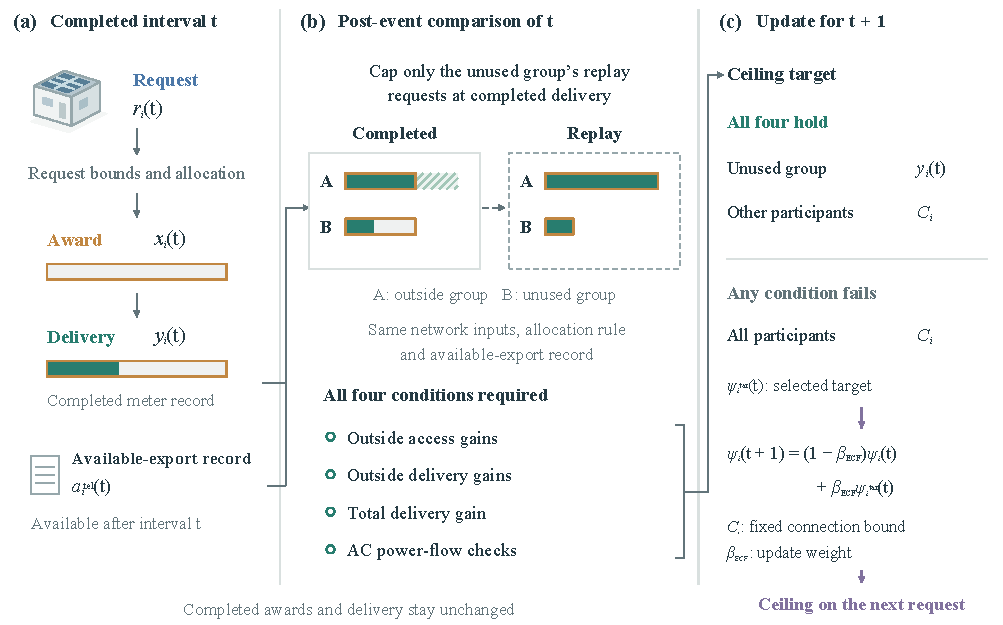
\includegraphics[width=\textwidth]{figures/fig02_ecf_framework.pdf}
\caption{Using completed delivery to update later request ceilings.
(a) Requests pass through connection bounds and current ceilings before the
existing allocation rule grants access in interval $t$.
(b) After delivery, only the unused-award group's replay requests are capped
at completed delivery. Exogenous network data, rule parameters, and the
available-export record stay fixed; awards and power flows are recalculated.
The bars follow Fig.~\ref{fig:problem_motivation}(c).
Qualification requires increased outside access, outside delivery, and total
delivery, together with the specified AC checks. Outside gains sum positive
changes; the total uses the signed system-wide change.
(c) A qualifying replay selects completed delivery as the unused group's
target and fixed connection bounds for everyone else. Otherwise, all targets
are fixed bounds. The gain $\beta_{\mathrm{ECF}}$ controls the move toward
each target. Only ceilings carry forward to $t+1$; completed awards and
delivery remain unchanged.}
\label{fig:claim_allocation_framework}
\end{figure*}

The comparison mechanisms test the delivery consequences of different updates
(Table~\ref{tab:feedback_controls}). Mismatch-only feedback uses a participant's
own delivery-to-award ratio without checking delivery elsewhere. The equal-total
control removes exactly as much total request as ECF in each interval but uses
a common proportional reduction for everyone. It therefore distinguishes the
amount of request removed from its distribution across participants.
Its matched total comes from ECF, making it an explanatory control rather than
an independently operated policy. Previous-day persistence provides
a further public-data comparison with more conservative requests.
Table~\ref{tab:experiment_evidence_map} links the resulting questions to the
experiments; Methods and the \suppref{} give their construction.

\begin{table}[!t]
\centering
\caption{ECF and comparison mechanisms. C denotes the controlled study and A
the Australian replay. Network data, allocation rule, and available-export
trajectory remain fixed within each comparison.}
\label{tab:feedback_controls}
\scriptsize
\setlength{\tabcolsep}{3pt}
\renewcommand{\arraystretch}{1.1}
\begin{tabularx}{\columnwidth}{@{}>{\raggedright\arraybackslash}p{1.65cm}>{\raggedright\arraybackslash}X>{\raggedright\arraybackslash}p{2.05cm}@{}}
\toprule
Mechanism & What changes & Question tested \\
\midrule
No feedback (C, A) & Requests are capped only by the fixed connection bound, without an adaptive ceiling. & Baseline delivery without a post-event update. \\
Shortfall-cost benchmark (C) & A modeled cost of non-delivery changes the participant's request choice before allocation. & How a stronger incentive changes requests and delivery. \\
Mismatch-only feedback (C) & A smoothed delivery-to-award ratio sets the next ceiling, without replay. & Whether own shortfall alone is a useful basis for updating access. \\
ECF without replay qualification (A) & The same ECF update applies after every unused award, with the same gain and capacity-recovery target. & Whether checking recoverable delivery adds value beyond the update formula. \\
Equal-total control (C, A) & One proportional factor removes the same total request as ECF at each interval. & Whether the distribution of request reduction matters. \\
Previous-day persistence (A) & The request uses previous-day available export with no forecast increment or replay. & Whether conservative requests save unused access at the expense of delivery. \\
ECF (C, A) & When all four replay conditions hold, the unused-award group's later ceilings move toward completed delivery. Other ceilings recover. & Whether selective use of completed records improves later delivery. \\
\bottomrule
\end{tabularx}
\end{table}

\begin{table}[!t]
\caption{Study questions, conclusions, and applicable scope}
\label{tab:experiment_evidence_map}
\centering
\scriptsize
\setlength{\tabcolsep}{3.0pt}
\renewcommand{\arraystretch}{1.13}
\begin{tabularx}{\columnwidth}{@{}>{\raggedright\arraybackslash}p{1.65cm}>{\raggedright\arraybackslash}X>{\raggedright\arraybackslash}p{2.0cm}@{}}
\toprule
Question & What the experiment establishes & Applicable scope \\
\midrule
When does an unused award displace delivery? & Controlled static comparisons
(Fig.~\ref{fig:endogenous_request_choice}) separate productive high requests
from cases in which the changed-request group obtains a higher combined modeled
payoff and a larger unused award while total delivery falls.
& Designed request comparisons under fixed network conditions. \\
What does selective feedback add? & Shortfall costs suppress both displacement
and useful delivery. At zero shortfall cost and the primary gain, ECF improves
mean delivery over mismatch-only feedback and equal-total reduction
(Figs.~\ref{fig:behavior_linked_trace}--\ref{fig:gain_and_replay}).
& Controlled profiles with exact simulated available-export records. \\
When can ECF help or harm? & Changing only the time order changes delivery;
unit gain can reverse the benefit. Delivery and allocation equality need not
move together (Figs.~\ref{fig:gain_and_replay}--\ref{fig:behavior_linked_physical_fairness}).
& Five rules within a declared synthetic envelope; all reported controlled
states pass the specified AC checks. \\
Does the delivery gain extend to public-data simulations? & The primary replay
increases delivery relative to no feedback and equal-total reduction
(Fig.~\ref{fig:australian_external_replay}). Gain, record, and cohort changes
show when that advantage persists or reverses
(Fig.~\ref{fig:australian_sensitivity}). & Published network and measured
profiles; constructed requests and modeled delivery. \\
What do the replay test and later response each contribute? & Qualification
improves delivery over the same update without it, but conservative recovery
tests do not always improve subsequent delivery
(Sections~\ref{sec:qualification_results}--\ref{sec:record_results};
SI S10.6, S10.8--S10.9, and S10.15).
& Paired network days; continuous memory within observed date blocks. \\
Who gains, and how do location and PV capacity matter? & Profile placement,
PV capacity, and topology change aggregate gains. Individual and section-level
gains are not universal (Fig.~\ref{fig:taxonomy_panel}; SI S10.10--S10.14). & Fixed participant locations in placement/capacity tests;
separate section, model, and participant outcomes. \\
\bottomrule
\end{tabularx}
\end{table}

\section{Results and discussion}
\label{sec:results}

Matching the total request reduction does not match delivered electricity.
At zero shortfall cost and gain 0.5, ECF delivers 24.8~kW more than the
equal-total control in the controlled study. The Australian public-data
simulation gives the same direction of change, with a 1.39-MWh advantage over
80 assessed days. The same daily simulation also tests whether the replay
criterion adds value beyond the update formula. Applying that formula after
every unused award leaves less authorization unused but delivers 6.42~MWh
less than ECF. Thus neither the total request reduction nor the amount of
unused authorization alone explains the delivery outcome.

The request-choice analysis first identifies when a larger request benefits
its sender at the expense of total delivery. Controlled comparisons then
examine which access is preserved by feedback and how this depends on the
allocation rule and timing. The public-data results distinguish the effects
of request distribution, the four replay conditions, and update weight. Unit gain
reverses the benefit, showing why finding recoverable delivery in a completed
interval is not enough to ensure a useful subsequent update. Physical checks
and equal-total matching are assessed separately from the delivery gains.

Controlled results report mean delivered power in kW. Their request-effect
comparisons subtract the forecast-based reference, whereas feedback comparisons
subtract the named control from ECF. The Australian replay reports modeled
energy in MWh, with smaller daily and section-level differences in kWh.
Positive feedback comparisons favor ECF; all differences are calculated before
rounding. Table~\ref{tab:experiment_evidence_map} gives the study map.

\long\def\EESexperimentalmethod{%
\subsection{Controlled multi-interval experiment}
\label{sec:case_setup}

The static experiment distinguishes productive larger requests from requests
that reduce total delivery. The multi-interval experiment then tests whether
ECF increases later delivery after an unused-award episode meets the four replay
conditions. Within each
matched comparison, we hold the allocation rule, exogenous network data,
reactive-power setting, and AC power-flow criteria fixed. The study combines the
network in Section~\ref{sec:network_ac} with the five rules in
Table~\ref{tab:policy_taxonomy}. Section S3 of the \suppref{} lists the temporal
sequences and the complete comparison design.

One conditional available-export tree links request choice to realized
delivery:
\begin{align}
    a_i^{(k)}(t)
    &=\min\!\left\{C_i,
\left(1+\sigma\varsigma_k\right)a_i^{\mathrm{fcst}}(t)\right\},
\label{eq:available_export_probability_tree}\\
(\varsigma_k)_{k=1}^{5}&=(-2,-1,0,1,2),\qquad
(\pi_k)_{k=1}^{5}=\frac{1}{16}(1,4,6,4,1).
\nonumber
\end{align}
The standardized support $(\varsigma_k)_{k=1}^{5}$ has weighted mean zero and
weighted variance one. The tested values of the dimensionless uncertainty scale
$\sigma$ keep $1+\sigma\varsigma_k$ nonnegative. Node $k$ occurs with
probability $\pi_k$, and the upper bound $C_i$ clips its available export. Thus,
the participant's forecast anchors both the ex-ante request choice and the
later available-export realization. Equation~\eqref{eq:endogenous_best_response}
selects the request multiplier from the grid in
Table~\ref{tab:behavior_design}.

The static experiment spans 30 participant locations, five allocation rules,
both reactive-power settings, five uncertainty levels, and nine normalized
shortfall-cost levels. The resulting 13,500 request-choice cases evaluate the
smallest payoff-maximizing multiplier and support the matched classification of
request increases before any temporal feedback is applied.

The multi-interval experiment carries the selected $\gamma_i^\star$ from the
corresponding static setting into a 16-interval trajectory. Each participant in
the changed-request set $\mathcal K$ submits
\begin{equation}
r_i^\star(t)=\gamma_i^\star(\vartheta,\sigma,\mathcal R,q_{\mathrm{pf}})
a_i^{\mathrm{fcst}}(t),
\label{eq:dynamic_endogenous_request}
\end{equation}
before available export is realized; participants outside $\mathcal K$ submit
their forecast requests. Three profiles contain the same support-node counts
and differ only in temporal order: clustered, intermittent, and
shock--recovery. Cyclic participant offsets prevent all participants from
realizing the same node at once. Because this is a controlled experiment, the
post-event record equals the simulated available export,
$\mathbf a^{\mathrm{tel}}(t)=\mathbf a(t)$.

The spatial cases change one participant, five electrically local participants,
or five dispersed participants. Every changed participant uses the multiplier
that maximizes its expected payoff in the corresponding single-participant,
single-interval calculation. The
five-participant cases therefore apply heterogeneous request changes
simultaneously. We compare the shortfall-cost benchmark, mismatch-only
feedback, three ECF gains, and the equal-total control. All 1,620 trajectories
are matched by allocation rule, temporal profile, changed-request set,
normalized shortfall cost, and reactive-power setting. Their 25,920 interval
comparisons preserve the same matching.

Table~\ref{tab:behavior_design} summarizes the controlled design; Section S3
of the \suppref{} gives the full trajectory construction and comparison counts.

\begin{table}[!t]
\caption{Controlled medium-voltage multi-interval design}
\label{tab:behavior_design}
\centering
\scriptsize
\setlength{\tabcolsep}{3.0pt}
\begin{tabularx}{\columnwidth}{@{}lX@{}}
\hline
Factor & Tested levels \\
\hline
Allocation rule & WP, ER, EA, ME, FA \\
Controlled feeder & 141-bus radial feeder; demand scale 0.70; 30 fixed participant buses \\
Reactive-power setting $q_{\mathrm{pf}}$ & Q0, Q95 \\
AC limits & $0.95\le v_b\le1.05$~pu; $\mathrm{LR}_\ell\le1$ using both branch ends \\
Request-choice grid $\Gamma$ & $\{1.0,1.1,\ldots,2.0\}$; smallest maximizer \\
Static uncertainty $\sigma$ & 0, 0.05, 0.10, 0.20, 0.30 \\
Static normalized shortfall cost $\vartheta$ & 0, 0.05, 0.10, 0.25, 0.50, 1, 2, 5, 10 \\
Dynamic $(\sigma,\vartheta)$ & $\sigma=0.20$; $\vartheta\in\{0,1,10\}$ \\
Temporal profile & Clustered, intermittent, shock--recovery \\
Changed-request set & One participant; local five; dispersed five \\
Comparison mechanism & Shortfall-cost benchmark; mismatch-only feedback $\beta_{\mathrm{ratio}}=0.5$; ECF $\beta_{\mathrm{ECF}}=0.25,0.5,1$; equal-total control \\
FA parameters & $\alpha_{\mathrm{FA}}=0.20$ MW; $\epsilon_{\mathrm{FA}}=10^{-6}$ MW; $\alpha_{\mathrm{FA}}$ sensitivity: $0.05,0.10,0.20,0.40,0.80$ MW \\
Controlled-study decision tolerances & $\epsilon_x=10^{-9}$ MW; $\tau_{\mathrm{rpl}}=\tau_E=2\times10^{-10}$ MW \\
Horizon & 16 intervals with exact tree frequencies \\
Sample size & 1,620 trajectories; 25,920 matched interval comparisons, each AC-checked \\
\hline
\end{tabularx}
\end{table}

}

\long\def\EESaustralianmethod{%
\subsection{Australian public-data replay}
\label{sec:australian_method}

The public-data replay combines two Australian sources. The first is a
published unbalanced OpenDSS model derived from an 11-kV feeder
\cite{geth2025australianfeeder}. It contains 1,255 service connections and 33
low-voltage sections, of which 30 carry mapped service loads. Its topology and
equipment data come from geographic information system records and documented
engineering completions.

The chronological source is the Ausgrid panel of 300 gross-metered solar homes
\cite{ausgrid2014solarhomes}. It provides half-hour gross PV generation, general
consumption, and controlled-load energy from July 2010 to June 2013. The profile
and network sources have no common customer identifier. We therefore use one
deterministic profile-to-service-point mapping. All 300 profiles are used before
any profile is reused. This primary mapping remains fixed within all primary
trajectories. A separate sensitivity uses five alternative placements of the
same profiles, as specified below.

The three source years serve separate roles. Data from 2010--2011 estimate a
half-hour-specific forecast increment from day-to-day changes. Data from
2011--2012 select the feeder load scale and qualify the allocation-stage
upper-voltage ceiling. Data
from 2012--2013 provide the later assessment trajectories. Let $d$ index
calendar days, and let $\tau\in\{1,\ldots,48\}$ index half-hours. We divide each
half-hour energy value by 0.5~h and 1,000 to obtain average power in MW.

The primary analysis retains source rows marked as actual. Estimated or
substituted gross generation and general consumption are excluded. Controlled
load is required whenever that customer-year contains the channel. We do not
impute missing values.

The request construction uses the previous calendar day. A network day is
eligible only when every distinct source profile used by the fixed mapping is
complete on both the current and previous calendar day and both dates pass the
chronology check. Reusing a source profile at several service points does not
repeat its completeness requirement. We also exclude Australian daylight-saving
transition dates from the state recursion. The assessment then contains 80
network-day trajectories, or 3,840 half-hours
per control. It includes 21 days in January, 11 in April, and 24 each in May and
June. No other assessment month contains an eligible day. A complete-customer
sensitivity retains customers with records in all three years under the same
loading assumptions.

The forward-uptake scenario assigns export participation to 418 of the 1,255
service connections. We scale the 300 PV profiles to a mean capacity of
9.9~kWp. Fixed profile reuse across 418 participants gives a participant mean
of 9.784~kWp.
The 9.9-kWp scale uses the reported mean Australian rooftop installation in the
March quarter of 2025 \cite{cer2025qcmrMarch}. This defines a forward uptake
case rather than a historical feeder reconstruction.

Let $\iota(i)$ denote the fixed profile mapping, and let
$\lambda_{\mathrm{PV}}$ and $\lambda_L$ denote the fixed PV and load scales.
After conversion to MW, $\mathrm{GG}$, $\mathrm{GC}$, and $\mathrm{CL}$ denote
gross PV generation, general consumption, and controlled load, respectively.
The scenario's profile-derived available-export proxy is
\begin{equation}
a_i^{\mathrm{prof}}(d,\tau)=\left[\lambda_{\mathrm{PV}}\,\mathrm{GG}_{\iota(i)}(d,\tau)
-\lambda_L\!\left(\mathrm{GC}_{\iota(i)}(d,\tau)+
\mathrm{CL}_{\iota(i)}(d,\tau)\right)\right]^+.
\label{eq:au_available_export_main}
\end{equation}
For control $c$, modeled connection-point delivery is
\begin{equation}
y_i^c(d,\tau)=\min\{x_i^c(d,\tau),a_i^{\mathrm{prof}}(d,\tau)\}.
\label{eq:au_delivery_main}
\end{equation}
The primary replay record is
$a_i^{\mathrm{tel}}(d,\tau)=a_i^{\mathrm{prof}}(d,\tau)$; record sensitivities
change only $a_i^{\mathrm{tel}}$. The profile-derived proxy represents
PV-minus-load surplus before network access is applied, so it can exceed $C_i$.
The bound limits the admitted request and export award, and hence
$y_i^c\le x_i^c\le C_i$; it does not clip the underlying proxy.

At each half-hour, the raw request begins with the previous day's
$a_i^{\mathrm{prof}}$ at the
same half-hour. It adds the positive part of the 90th percentile of
same-half-hour day-to-day changes estimated from 2010--2011, and then meets the
fixed connection bound $C_i$. This constructed forecast replaces the single-interval
request-choice model used in the controlled study. Household demand uses 0.95
lagging power factor, whereas PV export uses unity power factor.
For allocation, this retrospective replay treats contemporaneous half-hour
household demand as fixed exogenous data; load-forecast error is not modeled.

The Australian replay sets
$\epsilon_x^{\mathrm{AU}}=\tau_{\mathrm{rpl}}^{\mathrm{AU}}=2\times10^{-6}$~MW
(2~W). These are numerical thresholds for the unused-award and recovery tests,
not estimates of measurement accuracy. The controlled thresholds in
Table~\ref{tab:behavior_design} are smaller and serve its deterministic
calculations. Record uncertainty is treated separately through
$\delta_i$ or the stated sensitivity transformations. Section S3 of the
\suppref{} places both studies' thresholds side by side.

At each half-hour, an unbalanced nonlinear AC search scales the admitted request
as $x_i(d,\tau)=\rho r_i^{\mathrm{adm}}(d,\tau)$, with
$\rho\in[0,1]$. If the full request fails, zero-anchored bisection yields the
largest feasible lower-bracket factor encountered. This is a feasible-factor search; global maximality would additionally require
monotonic feasibility or a search of the full factor interval.
It stops when the factor bracket is at most $10^{-5}$ or after 24 iterations.
For every candidate, the load-only and authorized-export endpoints must
converge, remain above 0.90~pu, and satisfy native transformer nameplates; the
authorized endpoint must also remain below the 1.07-pu allocation-stage
upper-voltage ceiling. The profile-derived delivery state is screened against
the 0.90--1.10-pu physical voltage range and the same transformer limits.
Because the public model provides no usable native line ampacities, the physical
scope covers customer voltage and transformer loading.
Customer voltage is measured across each modeled service terminal: phase to
neutral for wye connections and phase to phase for delta connections. The
nonlinear solution tolerance is $10^{-10}$.

The scenario examines allocation of constrained export access under feasible
operating conditions. It uses a load multiplier of 0.30 and a 1.07-pu
upper-voltage ceiling during authorization, retaining 0.03~pu below the
1.10-pu physical upper limit. Feeder-setting comparisons use no-feedback
operation to check physical feasibility, retain useful delivery, and preserve
intervals in which network limits restrict requests. The selected settings
apply to all controls, sensitivities, nested sections, and representative
topologies. Delivery states are checked separately because an authorization
margin alone does not guarantee their feasibility.

In the primary comparison, each assessed day starts with $\psi_i(1)=C_i$.
The controls are no feedback,
previous-day persistence, ECF with $\beta_{\mathrm{ECF}}=0.5$, and the
equal-total control. Previous-day persistence uses the preceding day's
same-half-hour available-export proxy without the added forecast increment or
any replay. These comparisons retain state memory within each day.

The paired comparisons separate update qualification, memory, and information
quality. ECF without replay qualification retains the update formula and gain
0.5 but moves ceilings toward completed delivery after every unused award.
Each control evolves its own ceilings and deliveries under common raw requests
and network conditions (SI S10.6). The continuous-state comparison instead
carries ceilings across midnight within the ten observed blocks of 1--35 days.
It retains the three tested gains and starts a new block at capacity only
after a calendar gap (SI S10.8).

The record comparisons retain unperturbed availability for delivery assessment.
One set scales the post-event record by 0.9 or 1.1, delays it by one half-hour,
or replaces a deterministic 10\% of participant records with completed delivery.
All transformed records are floored at current modeled delivery; the first
lagged half-hour also uses delivery alone. Each setting generates its own
equal-total control. A second set compares point-record and lower-bound
recovery tests at error radii of 1\%, 5\%, and 10\% of registered capacity,
under common positive and negative biases. These controls evolve separately.
Reference availability checks their recovery decisions afterward; it does
not select their updates. The exact-record case and six bias settings per
treatment give 13 settings (SI S10.9). These are prescribed error tests, not
a calibration of instrument accuracy.

Gain sensitivities use $\beta_{\mathrm{ECF}}\in\{0.25,1.00\}$ around the
primary 0.5. The complete-customer cohort keeps the 0.30 load multiplier
while changing customer composition and the eligible calendar (SI S10.7).
A separate behavioral comparison lets participants revise request-choice
probabilities from their own completed delivery, carrying preferences and
ceilings across consecutive dates. Its fixed-probability comparison uses the
same candidate requests and random draws. Independently evolving controls
and the conditional equal-total shadow are distinguished in SI S10.15.

Spatial comparisons change profile placement, PV capacity, or network
structure separately. Five mappings reassign whole profiles within participant
and nonparticipant groups, preserving profile reuse, PV capacities and forecast
histories, participant locations, phase connections, and aggregate inputs
(SI S10.10). The capacity comparison keeps the original mapping and all 418
participant locations, scales gross PV and registered capacities by
0.50, 0.75, 1.00, 1.25, or 1.50, and recalculates net available export and
forecast increments under the same construction rule (SI S10.11).
These comparisons retain the primary dates, load scale, network limits,
gain, and initialization.

The network panels use 13 published LV sections of the parent collection and
nine representative Australian LV models \cite{geth2021lvtaxonomy}.
Each section has at least 20 mapped connections and five export participants.
Representative-model inclusion requires a convergent service-voltage check
with household injections set to zero, a usable native transformer nameplate,
and the specified minimum connection counts. Original phase connections are
retained. All panels apply the common chronology, mapping rule, controls, and
network-setting policy; SI S10.12--S10.13 report each network separately.

Energy is the sum of half-hour average power multiplied by 0.5~h. The
statistical unit is the paired network-day trajectory. Intervals, participants,
and nested LV sections remain observations within that trajectory. We report
paired-day bootstrap percentile intervals and dependent wild-bootstrap
intervals. The latter preserve short-range calendar dependence while retaining
all eligible days.
Section S10 of the \suppref{} gives the filtering, scenario construction,
energy identities, sensitivities, and topology results.

For control $c$, let $E_X^c$ denote authorized export energy over the eligible
panel, and let $E_Y^c$ denote delivered export energy. Section S10 gives their
half-hour sums and the unused-authorization identity.

The same nonlinear solves record source-terminal active power and circuit loss.
This shows how a change in connection-point delivery affects upstream exchange. Under
the OpenDSS convention, negative source power supplies the feeder. Positive
power is export toward the upstream system \cite{epriOpenDSSTotalPower}. Let
$E_{\mathrm{up}}^c$ be the half-hour source-energy sum for control $c$. A
positive paired change means less upstream import or more upstream export.
Circuit loss is reported separately. Because the model contains
voltage-dependent passive elements, reported circuit loss need not equal the
entire difference between connection-point delivery and source-terminal exchange.
}

\subsection{Private delivery gains can accompany a larger loss elsewhere}
\label{sec:behavioral_results}

Larger requests can benefit the requesting participant while reducing total
delivery. Across 1,500 controlled parameter--location cases without a shortfall
cost, the participant gains 5.2~kW of expected delivery on average while others
lose 18.8~kW. Total delivery falls by 13.5~kW. The request model values the
participant's own gain but does not include the larger loss elsewhere. Because
the same uncertain-output model determines both request choice and expected
delivery, this difference arises from the allocation response rather than from
unrelated request and output curves.

Fig.~\ref{fig:endogenous_request_choice} shows how this response changes with
forecast uncertainty $\sigma$ and normalized shortfall cost $\vartheta$.
The latter is the modeled cost per unit of unused award divided by the value
per unit of delivered export. We compare weighted proportional (WP), equal
reduction (ER), equal access (EA), maximum export (ME), and fairness-aware (FA)
allocation under two reactive-power settings. Each selected request is paired
with the same participant's forecast-based reference. Methods gives the
five-outcome available-export model and exact finite-difference calculation.

The aggregate loss does not make every larger request unproductive. We classify
a request--access--delivery externality when expected payoff and unused award
both rise while total delivery falls. A productive high request instead raises
payoff without lowering total delivery beyond the numerical tolerance. For
$\vartheta\ge0$, the externality conditions imply that the requesting
participant delivers more and others lose still more; Methods and Section S2
of the \suppref{} prove this implication and specify the classification.

Both high-request classes occur in Fig.~\ref{fig:endogenous_request_choice}.
Among the 1,500 controlled parameter--location cases at $\vartheta=0$, pooled
over all five uncertainty levels, 71.5\% meet the
externality definition and 11.9\% are productive high requests. Reference
requests account for 14.7\%, and the remaining 1.9\% are larger requests that
meet neither high-request definition. Section S2 reports the corresponding
counts. The coexistence of these classes explains why request size alone is
insufficient to identify a delivery loss.

Uncertainty and the normalized shortfall cost shift the relative frequency of
these outcomes in opposite directions. With greater forecast uncertainty, a
large award can accommodate a higher-output realization. Greater $\vartheta$ makes
unused awards more costly, so the selected request falls. At $\vartheta=10$,
10.7\% of the 1,500 cases meet the externality definition. Across all cases, the
mean total-delivery loss, counting cases without a loss as zero, falls to
0.6~kW. Productive high requests still account for 11.5\% of the cases. A
shortfall cost can therefore reduce requests that lower total delivery while
preserving some productive requests above the forecast.

Panel (d) asks how much delivery is lost elsewhere per extra unit of unused
award. For each 0.1 increase in the request multiplier, it divides the first
quantity by the second. This ratio also gives the normalized shortfall cost
that would align the participant's payoff change with the total-delivery
change. Methods denotes it $\vartheta_{i,\Delta}^{\mathrm{ext}}$ and derives its
relation to the local marginal cost. The calculation covers 4,608 steps in
which own delivery and unused award rise while total delivery falls. The median
ratio is 2.29, with an interquartile range of 1.10--5.72. Rule-specific medians
range from 0.92 for ME to 5.37 for EA. This spread shows that one system-wide shortfall cost cannot
match the cross-participant delivery effect across all tested electrical
locations and operating states. It motivates the post-event feedback comparison
in the next section.

\begin{figure}[!t]
\centering
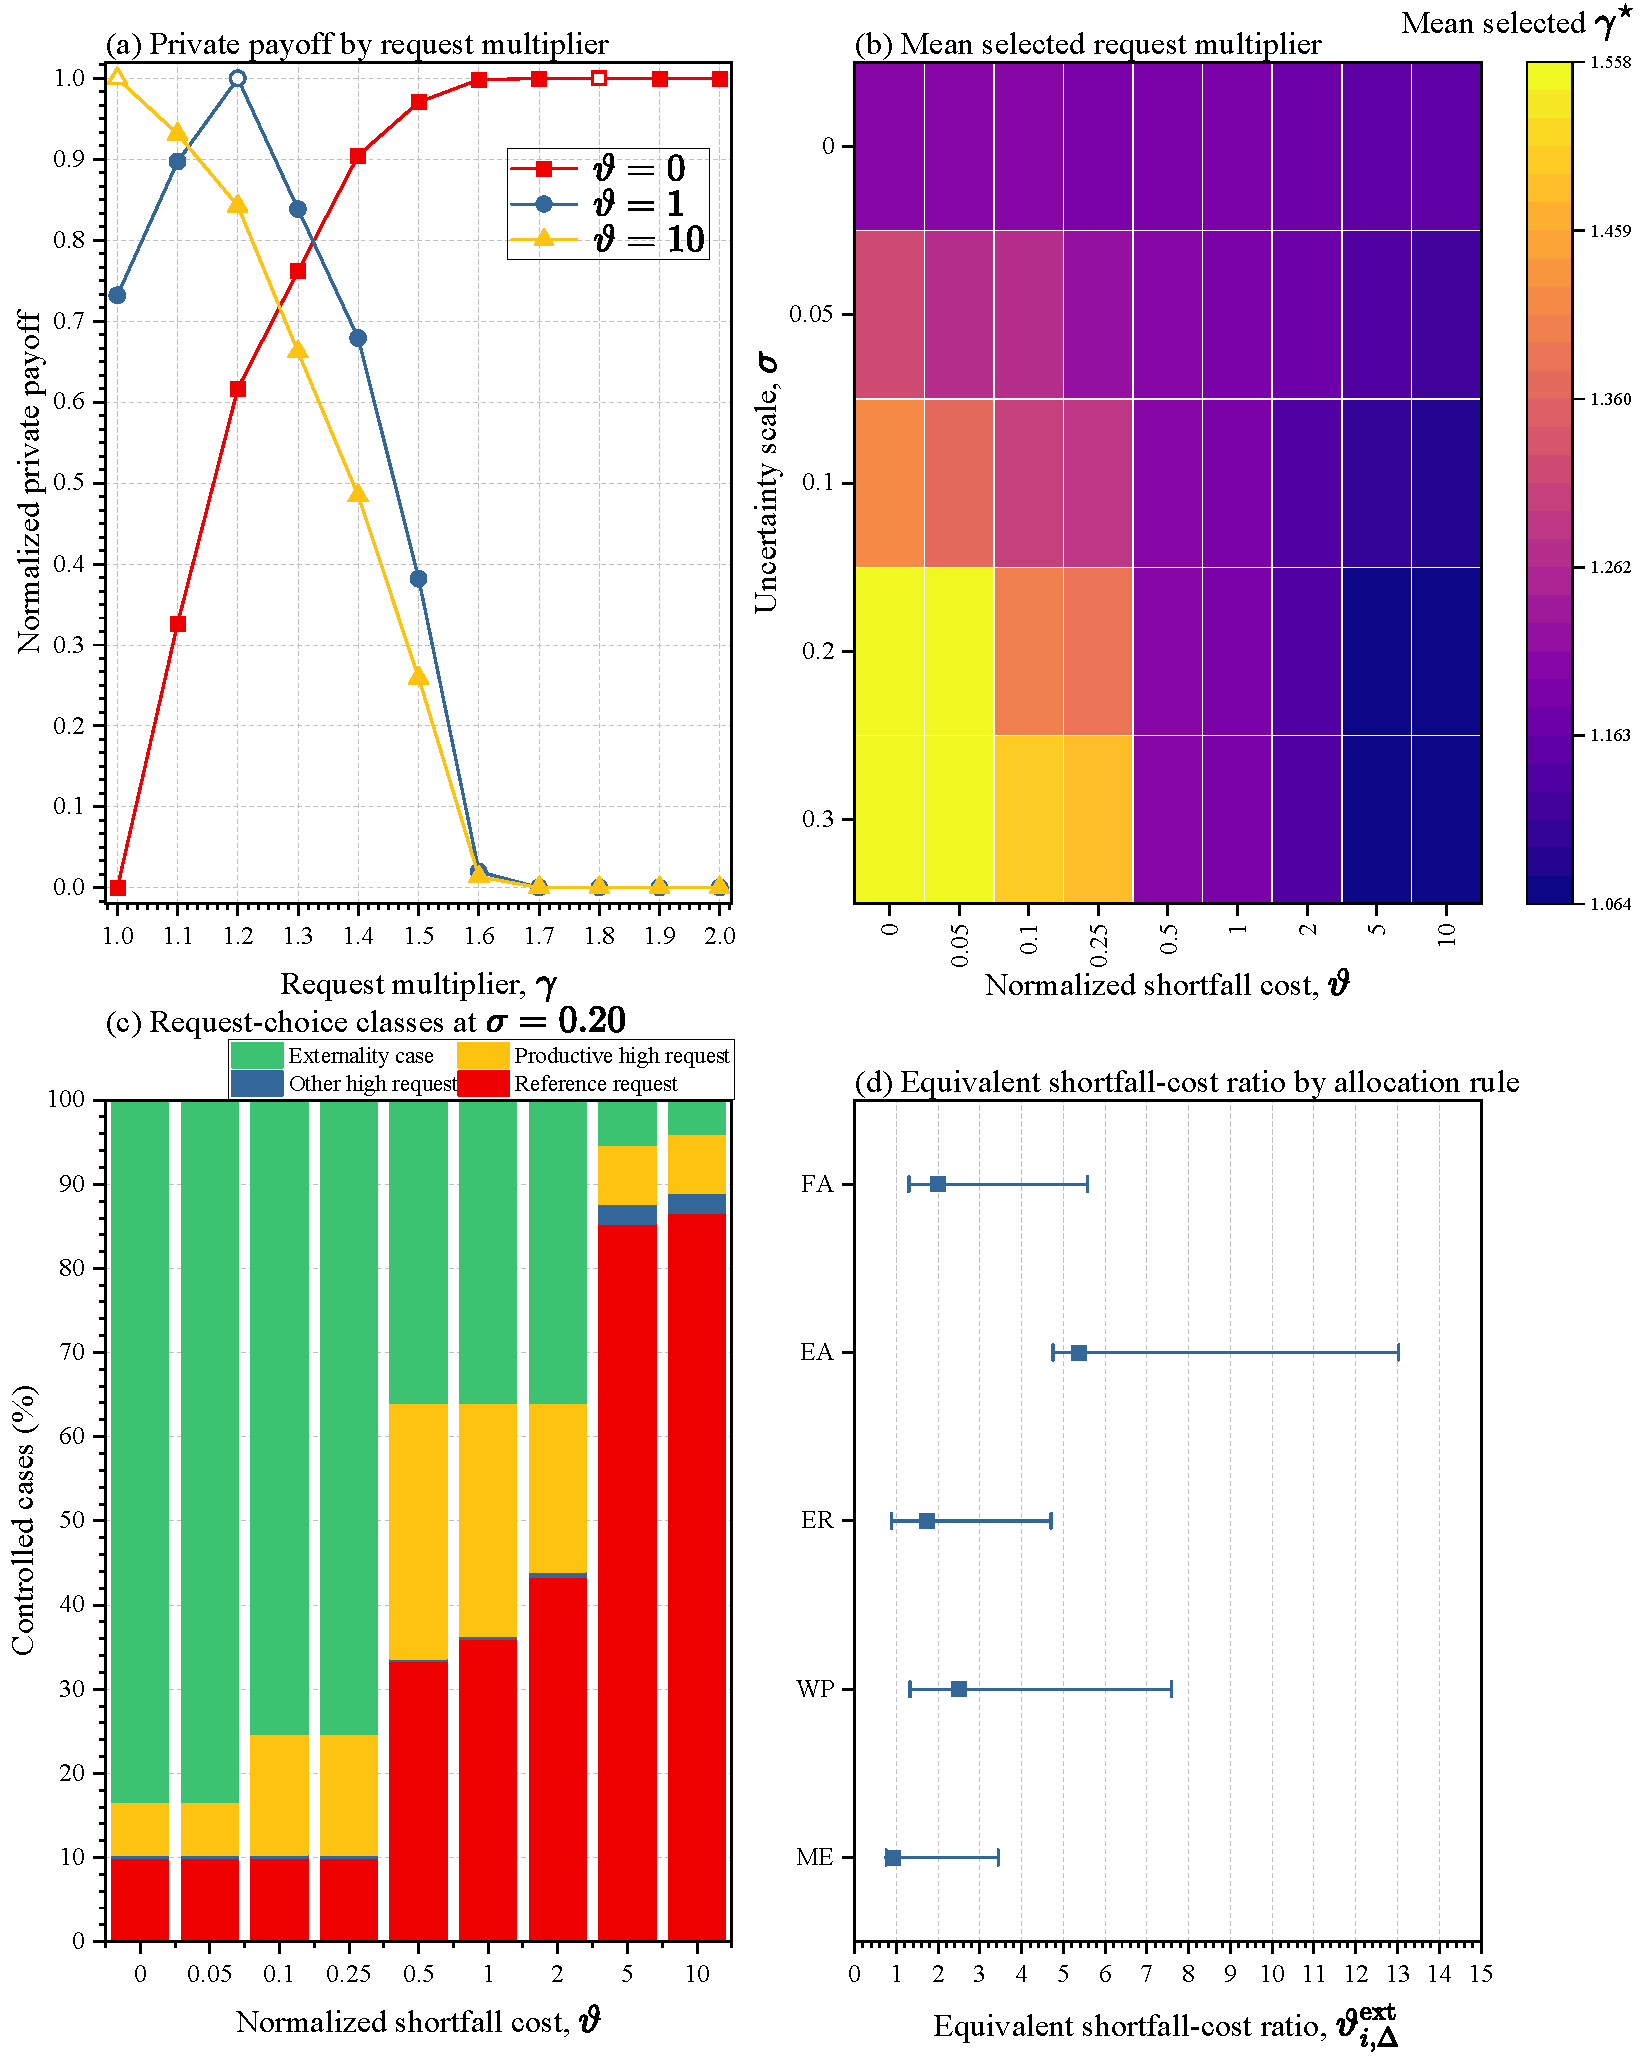
\includegraphics[width=\columnwidth]{figures/fig03_endogenous_request_choice.pdf}
\caption{How a larger request becomes productive or harmful before feedback.
(a) Representative private-payoff curves for three normalized shortfall-cost
levels.
Within each curve, payoff is rescaled as
$(U-U_{\min})/(U_{\max}-U_{\min})$; a zero span is plotted as zero.
(b) Mean selected request multiplier for each uncertainty and shortfall-cost
setting.
The mean covers participants, allocation rules, and reactive-power settings.
 (c) Shares at $\sigma=0.20$ ($n=300$): reference requests; productive high
 requests, which raise payoff without lowering total delivery; request--access--delivery
 externality cases, which raise payoff and unused awards while lowering total
 delivery; and other high requests, which meet neither high-request definition.
 (d) Finite-difference
cost ratio $\vartheta_{i,\Delta}^{\mathrm{ext}}$: expected delivery loss elsewhere per unit
increase in expected unused award for a 0.1 request-multiplier step. Squares show
rule-specific medians, and bars show interquartile ranges. WP, ER, EA, ME, and
FA denote weighted proportional, equal reduction, equal access, maximum export,
and fairness-aware allocation, respectively.}
\label{fig:endogenous_request_choice}
\end{figure}

\subsection{Selective updates preserve delivery that broad reductions remove}

At $\beta_{\mathrm{ECF}}=0.5$ and $\vartheta=0$, ECF delivers 24.8~kW more on
average than the equal-total control. Thus its advantage over uniform reduction
cannot be explained by removing more total request. The shortfall-cost and
mismatch-only comparisons ask whether request incentives or own delivery
provide the same benefit. A representative trajectory first shows the timing
needed to interpret these comparisons: feedback changes a later allocation,
not the completed interval used for the replay.
All dynamic controls start from the same raw requests and allocation in the
first interval. The changed-request group is
fixed for each trajectory, whereas the unused-award group is identified anew
after each interval and determines whose requests ECF caps in the replay.
Fig.~\ref{fig:claim_allocation_framework} shows the
timing, and Methods and Section S3 of the \suppref{} define the update.

\subsubsection{Completed delivery affects later access}

Feedback acts with a delay: it cannot change the interval whose shortfall
prompted the update. This is visible in the representative trajectory in
Fig.~\ref{fig:behavior_linked_trace}, where the controls start from the same
allocation and diverge only after a completed record becomes available. The three
16-interval profiles use standardized forecast deviations $-2,-1,0,1,2$
with counts $1,4,6,4,1$. They differ only in order: clustered groups the low
states, intermittent separates them, and shock--recovery places a low-output
episode between initial normal output and recovery. Participant offsets retain
these counts while preventing perfectly synchronized output. Section S3 gives
the exact sequences.

Fig.~\ref{fig:behavior_linked_trace} follows one trajectory in which five
electrically nearby participants change their requests and the available-export
states follow a shock--recovery ordering. It uses WP allocation, zero participant
reactive power (Q0), and $\vartheta=0$. An unused award first supplies the
candidate for replay; a feasible increase in delivery then supports a later
ceiling adjustment. The distinction between panel (c)'s completed-state recovery
and panel (d)'s later delivery is important: the former justifies attempting an
update, whereas the latter measures its outcome after available export changes.

\begin{figure}[!t]
\centering
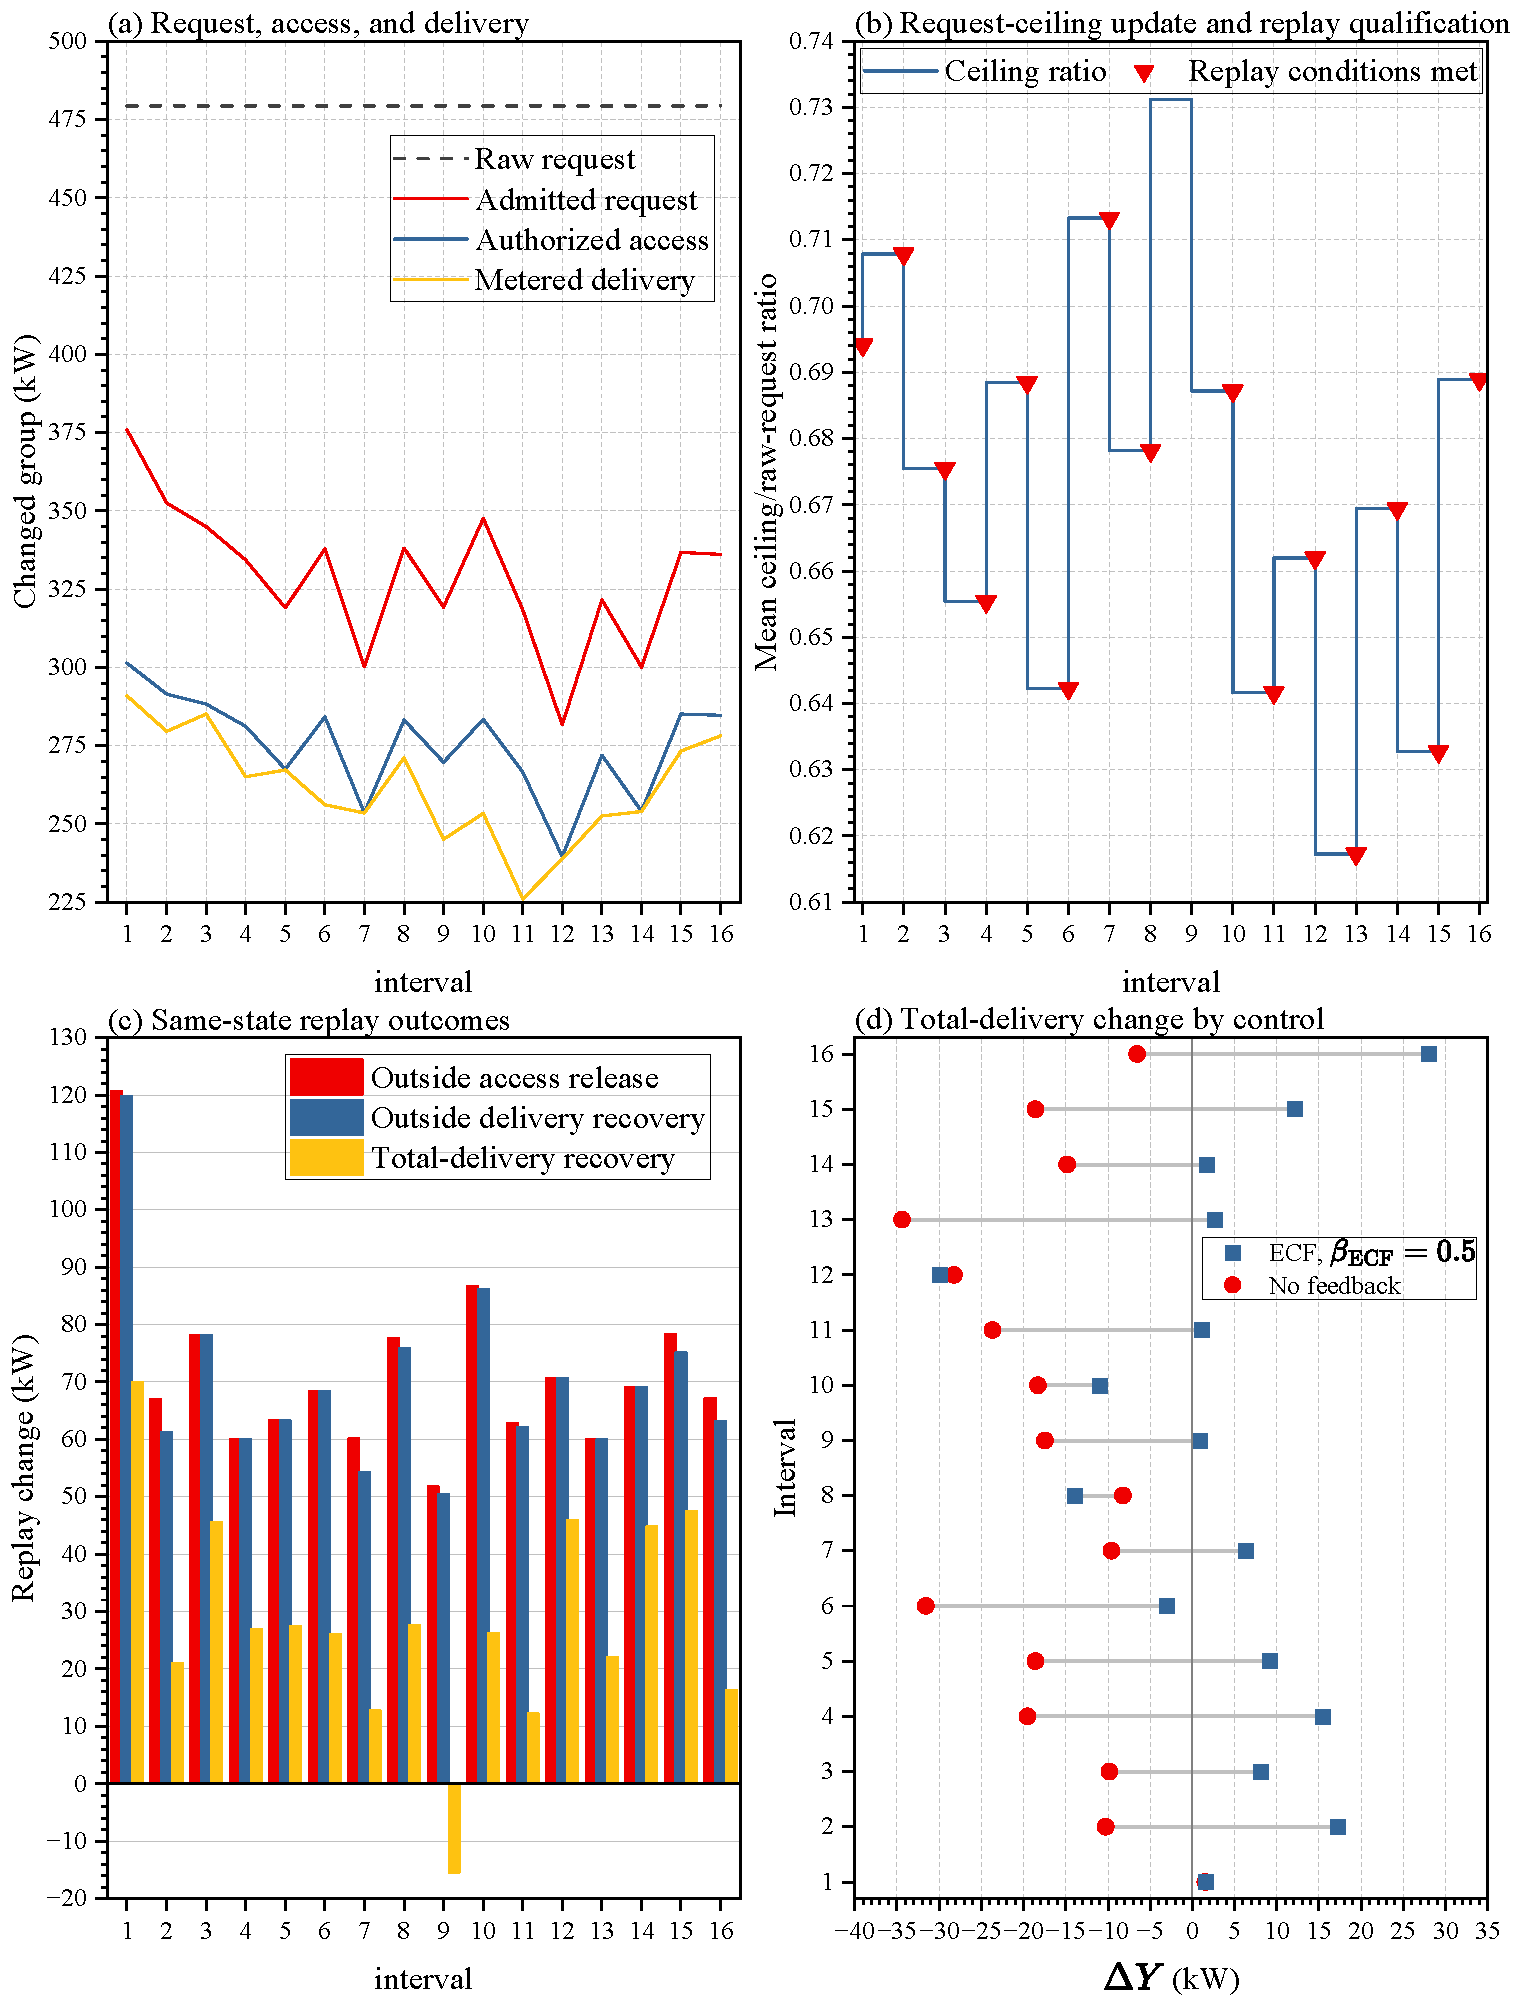
\includegraphics[width=\columnwidth]{figures/fig04_behavior_linked_temporal_trace.pdf}
\caption{One 16-interval ECF trace for the local-five, shock--recovery, WP--Q0
case at $\vartheta=0$. (a) Raw request, admitted request, awarded access, and
metered delivery for the changed-request group. (b) Mean ceiling-to-raw-request ratio
after each update. Red triangles mark intervals that meet the replay conditions.
(c) Access released and delivery recovered outside the current unused-award group, with the signed
change in total delivery. (d) Total-delivery change under ECF and no feedback.
The controls coincide in interval 1 because no earlier meter record exists.
The local-five case changes five electrically nearby participants;
shock--recovery is one 16-interval ordering of the same available-export-node
frequencies. WP denotes weighted proportional allocation, and Q0 sets
participant reactive power to zero.}
\label{fig:behavior_linked_trace}
\end{figure}

\subsubsection{A shortfall cost reduces displacement but also useful delivery}

An anticipated shortfall cost reduces the incentive to request unused access,
but also gives up some delivery during high-output intervals
(Fig.~\ref{fig:penalty_feedback_factorial}). We measure that trade-off against
forecast-based reference requests. The externality-interval share counts the
economic classification defined above; ECF activation counts a different event,
the completed-state replay meeting its four conditions.

With the shortfall cost alone, raising $\vartheta$ from 0 to 1 lowers the mean
request multiplier from 1.51 to 1.14. The externality-interval share falls from
50.1\% to 15.6\%, and delivery loss outside the changed-request group falls from
37.6 to 9.4~kW. The cost also removes 45.6\% of that group's delivery gain,
reducing it from 15.9 to 8.7~kW. At $\vartheta=10$, no interval meets the
externality definition, but the group's gain is only 0.07~kW. A strong shortfall cost therefore reduces
requests associated with delivery loss elsewhere, but it also removes useful
access when available export is unexpectedly high.

At $\vartheta=0$, the shortfall-cost benchmark coincides with no feedback.
Using that common baseline, mismatch-only feedback increases mean total
delivery by 15.2~kW, while ECF increases it by 24.9~kW. ECF's additional
advantage over mismatch-only feedback is therefore 9.7~kW. The three controls
receive the same raw requests. Relative to forecast-based reference requests,
the no-feedback loss of 21.7~kW becomes a gain of 3.2~kW under ECF. ECF retains
79.4\% of the changed-request group's no-feedback delivery gain and reduces
the delivery loss outside that group to 9.4~kW. The externality-interval share
falls by 29.0 percentage points. Section S3 reports the group decomposition and
the control comparisons with their respective baselines.

A gain in average delivery can coexist with more intervals classified as
request--access--delivery externalities because a count does not reflect the
magnitude of delivery changes. At $\vartheta=1$, ECF increases total delivery by 7.7~kW relative
to the shortfall-cost benchmark and lowers the externality-interval share by 6.7
percentage points. At $\vartheta=10$, the benchmark already has no externality
interval. Adding ECF raises the share to 1.3\%, although mean delivery still
increases relative to that benchmark. Feedback can therefore improve average
delivery even when that economic classification becomes more frequent.

\begin{figure}[!t]
\centering
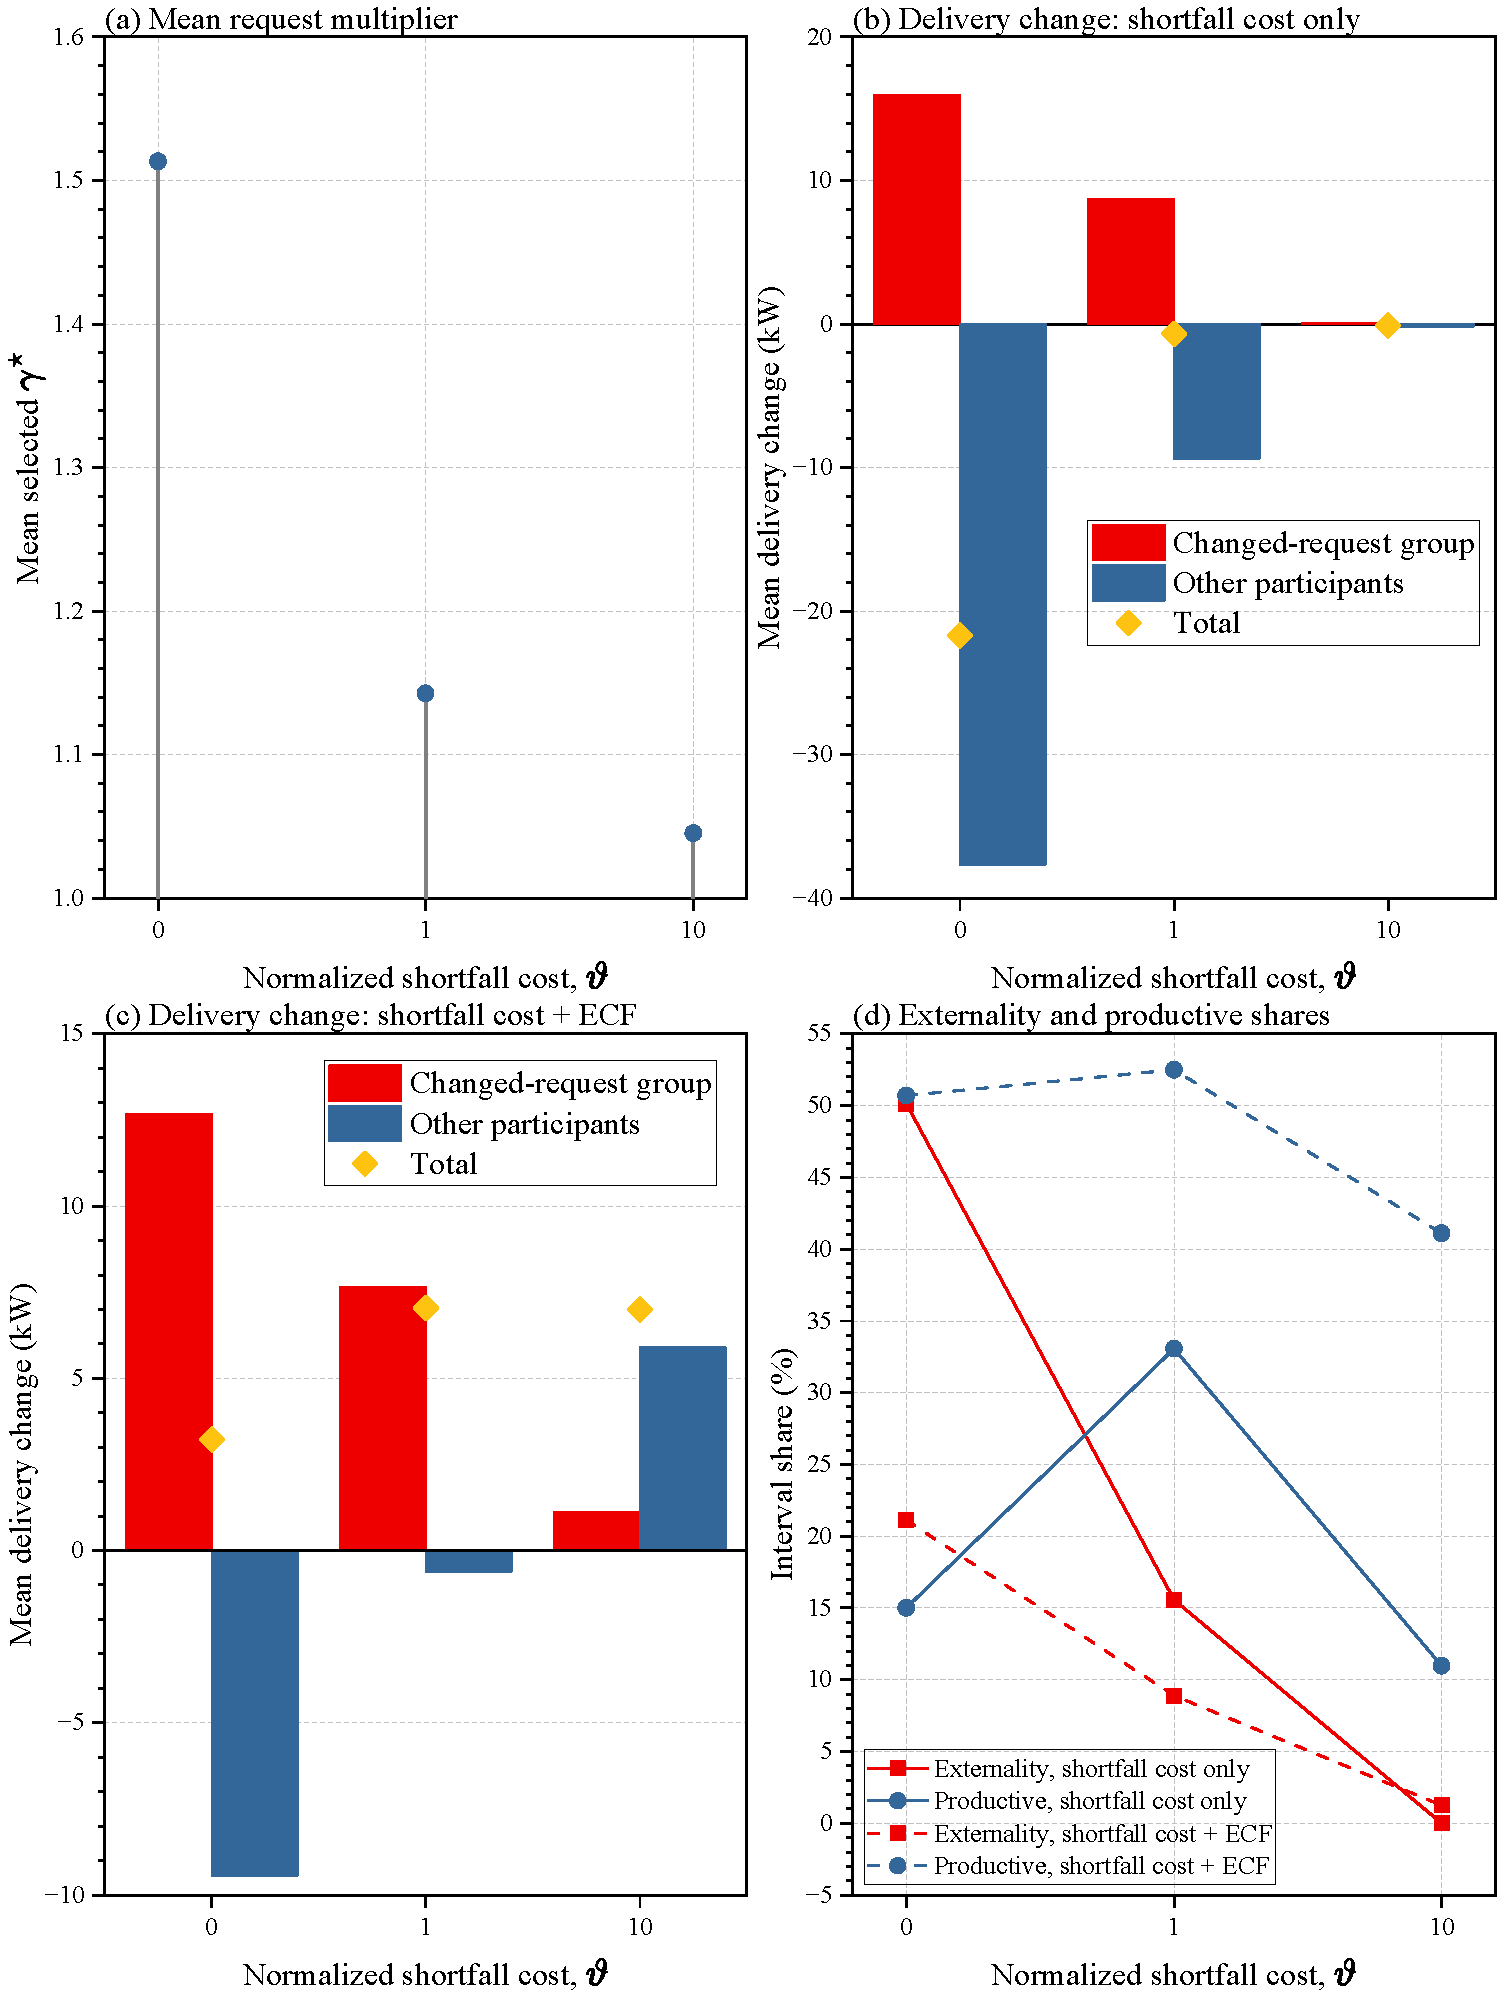
\includegraphics[width=\columnwidth]{figures/fig05_penalty_feedback_factorial.pdf}
\caption{How a modeled pre-allocation shortfall cost and post-delivery ECF affect
requests and delivery. Results cover all profiles, spatial cases, allocation
rules, and reactive-power settings. (a) Mean selected request multiplier.
(b) Delivery changes with the shortfall cost alone. The bars separate the
changed-request group and other participants; diamonds show their total. (c) The same
changes with the shortfall cost and ECF at $\beta_{\mathrm{ECF}}=0.5$. Positive blue bars denote
recovery outside the changed-request group. (d) Externality and productive-high-request
shares with and without ECF.}
\label{fig:penalty_feedback_factorial}
\end{figure}

\subsubsection{Where requests are reduced determines recovered delivery}

ECF and the equal-total control remove the same total request in every interval
but reduce different participants' requests. The comparison holds the allocation
rule, exogenous network conditions, and available output fixed. It measures
the delivery effect of the request distribution produced by ECF relative to
proportional reduction. Both electrical location and the output available at
each connection contribute to that effect. Mismatch-only feedback provides a
separate comparison with an update based on own delivery, without testing
recovery elsewhere. It changes both the information used and the update law,
whereas the equal-total control fixes the amount removed. The two comparisons
therefore assess the resulting updates from complementary directions.

At $\vartheta=0$ and $\beta_{\mathrm{ECF}}=0.5$, ECF delivers 9.7~kW more than
mismatch-only feedback and 24.8~kW more than the equal-total control.
ECF delivers more in 73.3\% and 95.6\% of the matched trajectories
($n=90$ for each comparison),
respectively. At $\vartheta=1$, the mean advantages are 6.8 and 9.0~kW. At
$\vartheta=10$, they are 6.8 and 8.2~kW. The advantage over both controls thus
persists across the three tested shortfall-cost settings.

\paragraph{A favorable replay does not guarantee a favorable later update.}
The feedback gain controls how much weight the latest interval receives.
Delivery changes nonmonotonically with that weight. At $\vartheta=0$, the mean
change relative to forecast-based requests is $-2.8$~kW for
$\beta_{\mathrm{ECF}}=0.25$. It rises to 3.2~kW at 0.5 but falls to $-23.4$~kW
at 1. The same reversal occurs at
$\vartheta=1$ and 10. The replay evaluates a completed output realization,
whereas the resulting ceiling applies to a different interval. At unit gain,
the previous ceiling is discarded in favor of that completed interval's target.
The negative response establishes the importance of this temporal distinction;
it does not by itself identify a single cause of the reversal. We use 0.5 as
the primary intermediate update weight, which gives the largest mean delivery
among the three tested gains in all three shortfall-cost settings.

The controlled study uses the exact available-export record in
Assumption~\ref{ass:post_event_available_export_record}; here, that record equals the
simulated available export. Of 12,960 replay attempts, 12,910
meet all four conditions. Among these intervals, median total-delivery
recovery is 37.8~kW. The interquartile range is 25.6--57.5~kW, and 99.5\%
of recoveries exceed 5~kW. At $\beta_{\mathrm{ECF}}=0.5$, 20 of 4,320 attempts
do not meet the conditions because total delivery does not rise. An unused award
therefore initiates a replay but does not by itself lower a later request ceiling.
These controlled trajectories combine larger requests with constrained export
access, so the replay usually finds delivery that could be recovered elsewhere.
The Australian replay has a lower activation rate of 12.6\%. The two rates
describe how often the four conditions hold in their respective experiments.

Fig.~\ref{fig:gain_and_replay} reports the gain sweep, paired control
comparisons, and replay-recovery distribution behind these main comparisons.

\begin{figure}[!t]
\centering
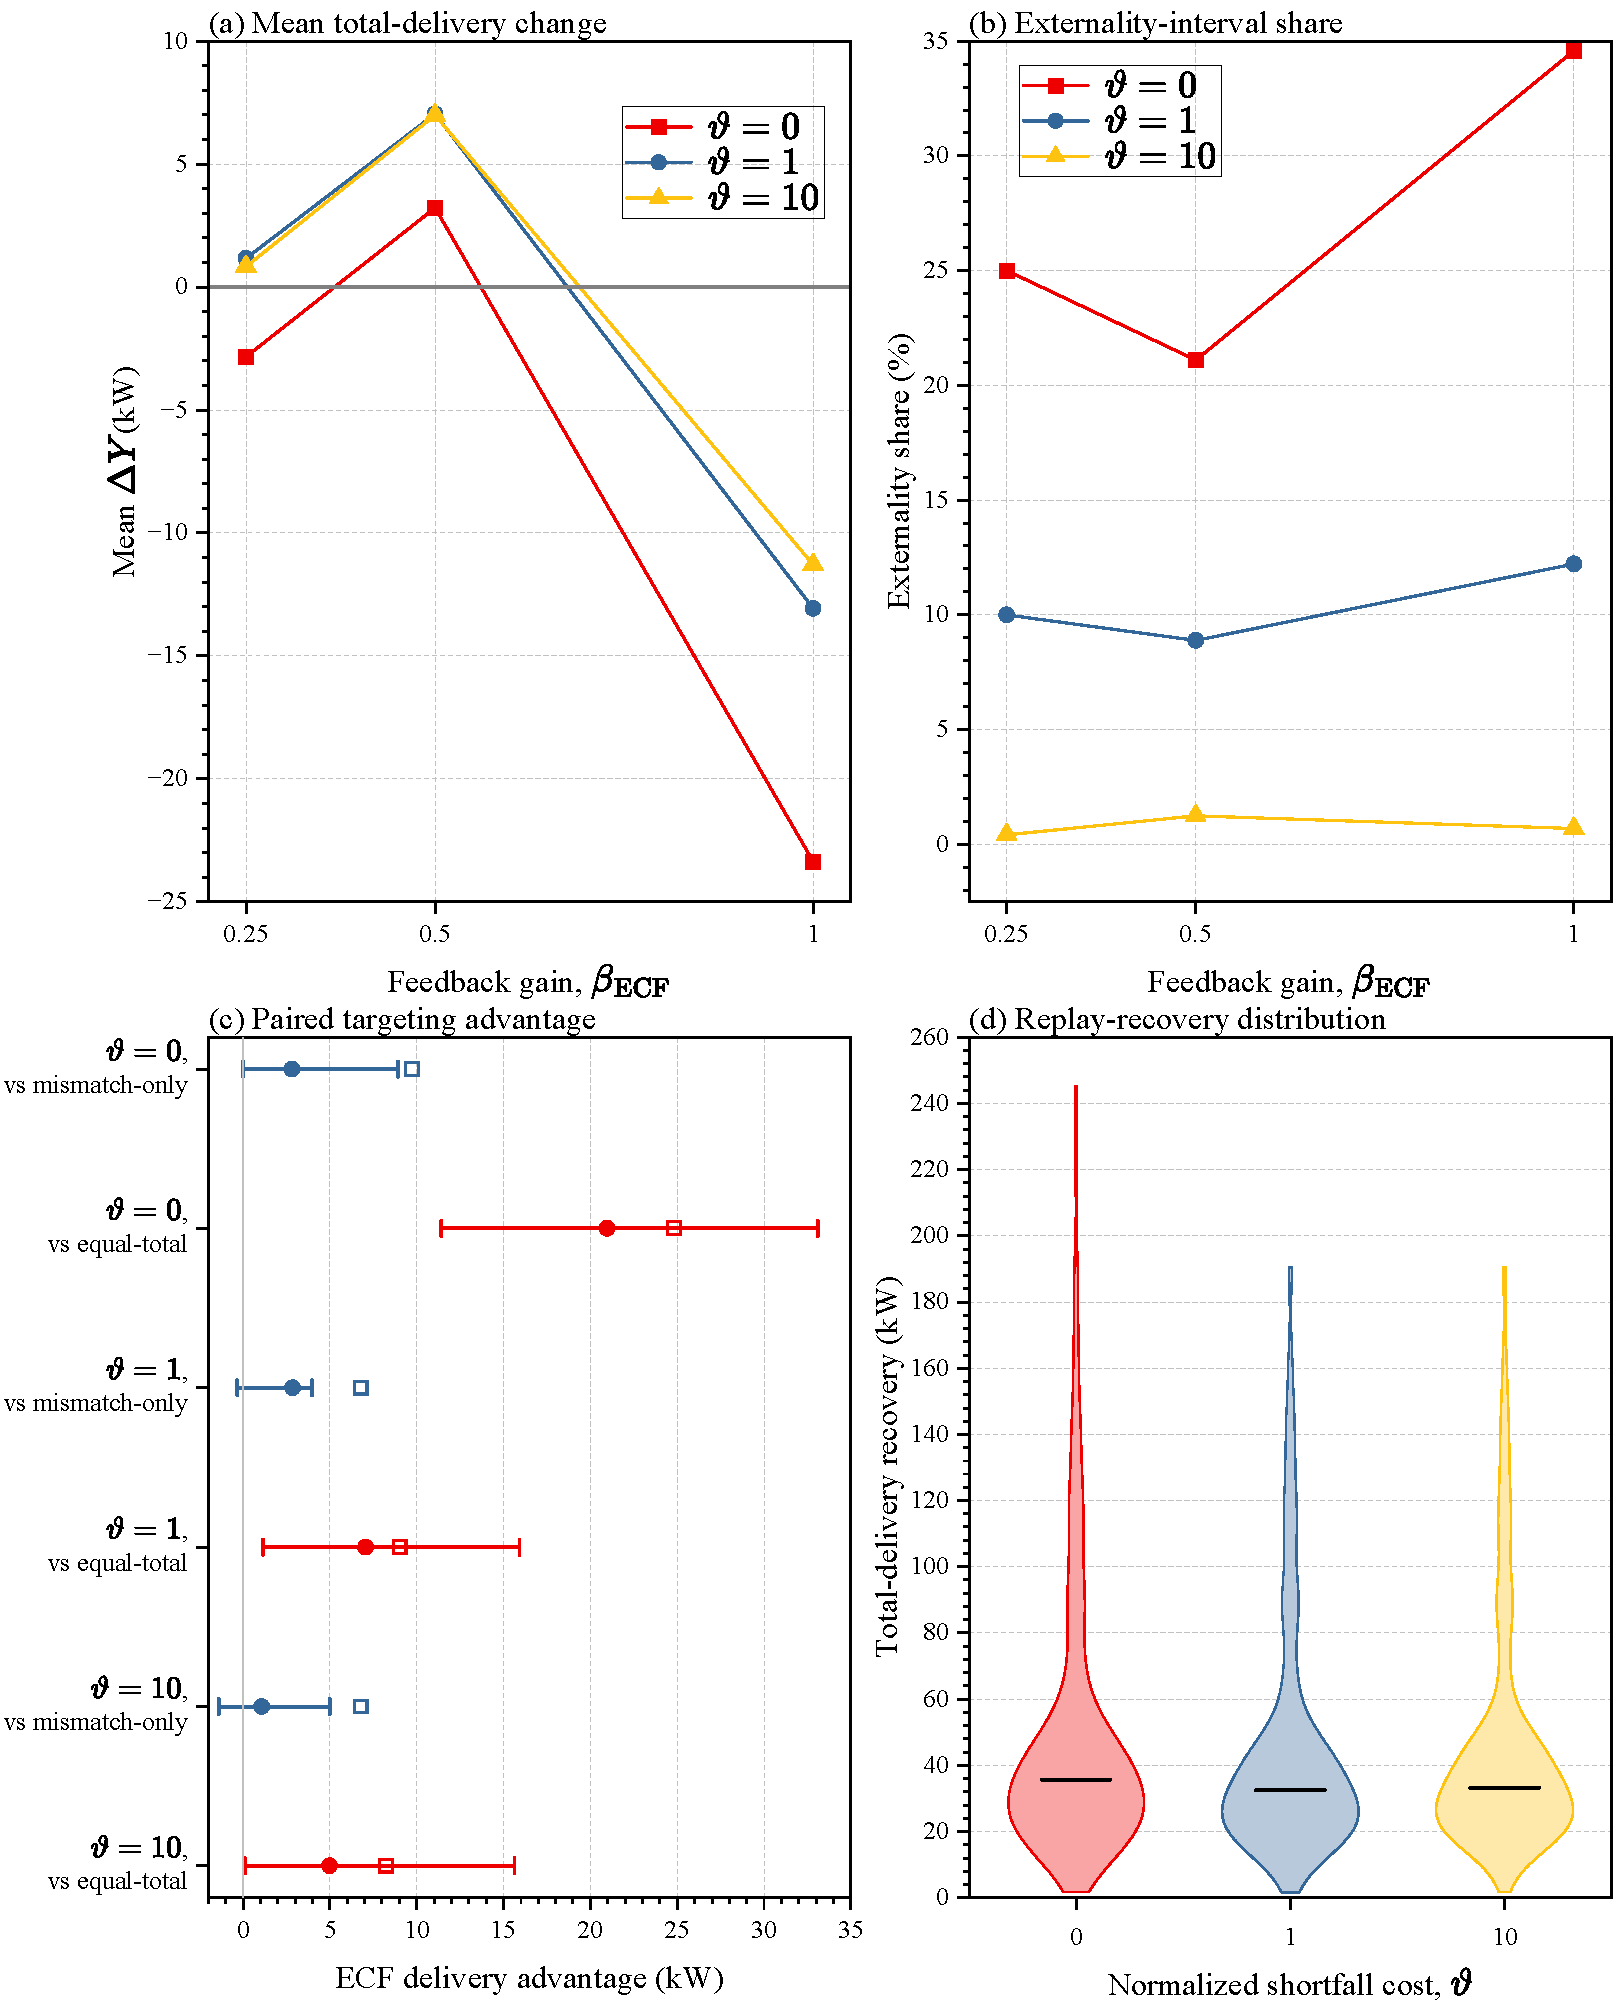
\includegraphics[width=\columnwidth]{figures/fig06_gain_and_replay.pdf}
\caption{Feedback-gain response, paired controls, and replay recovery across all
controlled dynamic cases. (a) Mean signed change in total delivery and
(b) externality-interval share for the three tested feedback gains. The series
denote $\vartheta=0,1,10$. (c) ECF delivery advantage in matched trajectories.
Rows labelled ``vs mismatch-only'' compare ECF with mismatch-only feedback. Rows
labelled ``vs equal-total'' compare ECF with the equal-total control.
Panel (c) uses the primary gain, $\beta_{\mathrm{ECF}}=0.5$.
Filled circles show medians, open squares show means, and whiskers show
interquartile ranges. The gray line marks zero. (d) Distribution of total
delivery recovered when the replay meets all four conditions. Violin width shows
empirical density, and the black horizontal segment shows the median.}
\label{fig:gain_and_replay}
\end{figure}

\subsection{Timing and allocation change the size of the delivery gain}

At $\vartheta=0$ and $\beta_{\mathrm{ECF}}=0.5$, the mean ECF delivery
advantage is positive at every factor level reported in
Fig.~\ref{fig:temporal_spatial_scaling}. This holds for every allocation rule,
temporal profile, spatial case, and reactive-power setting.
Against no feedback, the rule-specific gain ranges from 8.9~kW for FA to 67.5~kW
for EA. Against the equal-total control, it ranges from 9.7
to 50.8~kW. The positive direction is therefore not confined to one
allocation rule.

The three temporal profiles contain the same available-export values and frequencies.
Only their order changes. The mean delivery advantages over no feedback are
35.3~kW for the clustered profile, 12.2~kW for the intermittent profile,
and 27.3~kW for shock--recovery. Against the equal-total control, the
corresponding advantages are 34.4, 12.6, and
27.4~kW. Because each profile preserves the available-export values and their
frequencies, these differences isolate temporal ordering rather than a change
in the uncertainty distribution. A completed low-output interval has a different
value for later access when similar states are clustered than when they are
separated by other output states.

The mean delivery advantage over no feedback is 11.2~kW when one participant
changes its request. It is 35.0~kW for five electrically local participants
and 28.6~kW for five dispersed participants. Every participant still selects its own request
multiplier. The local--dispersed comparison holds group size fixed but changes
participant identities, electrical locations, and participant-specific
multipliers. The difference therefore reflects the selected participants as
well as their electrical placement. At the reported precision, zero reactive
power (Q0) and 0.95-power-factor absorption (Q95) both give a 24.9-kW mean
advantage over no feedback. Both also give a 24.8-kW mean advantage over the
equal-total control. The two comparator-specific results are
therefore unchanged across the two tested reactive-power settings.

\begin{figure}[!t]
\centering
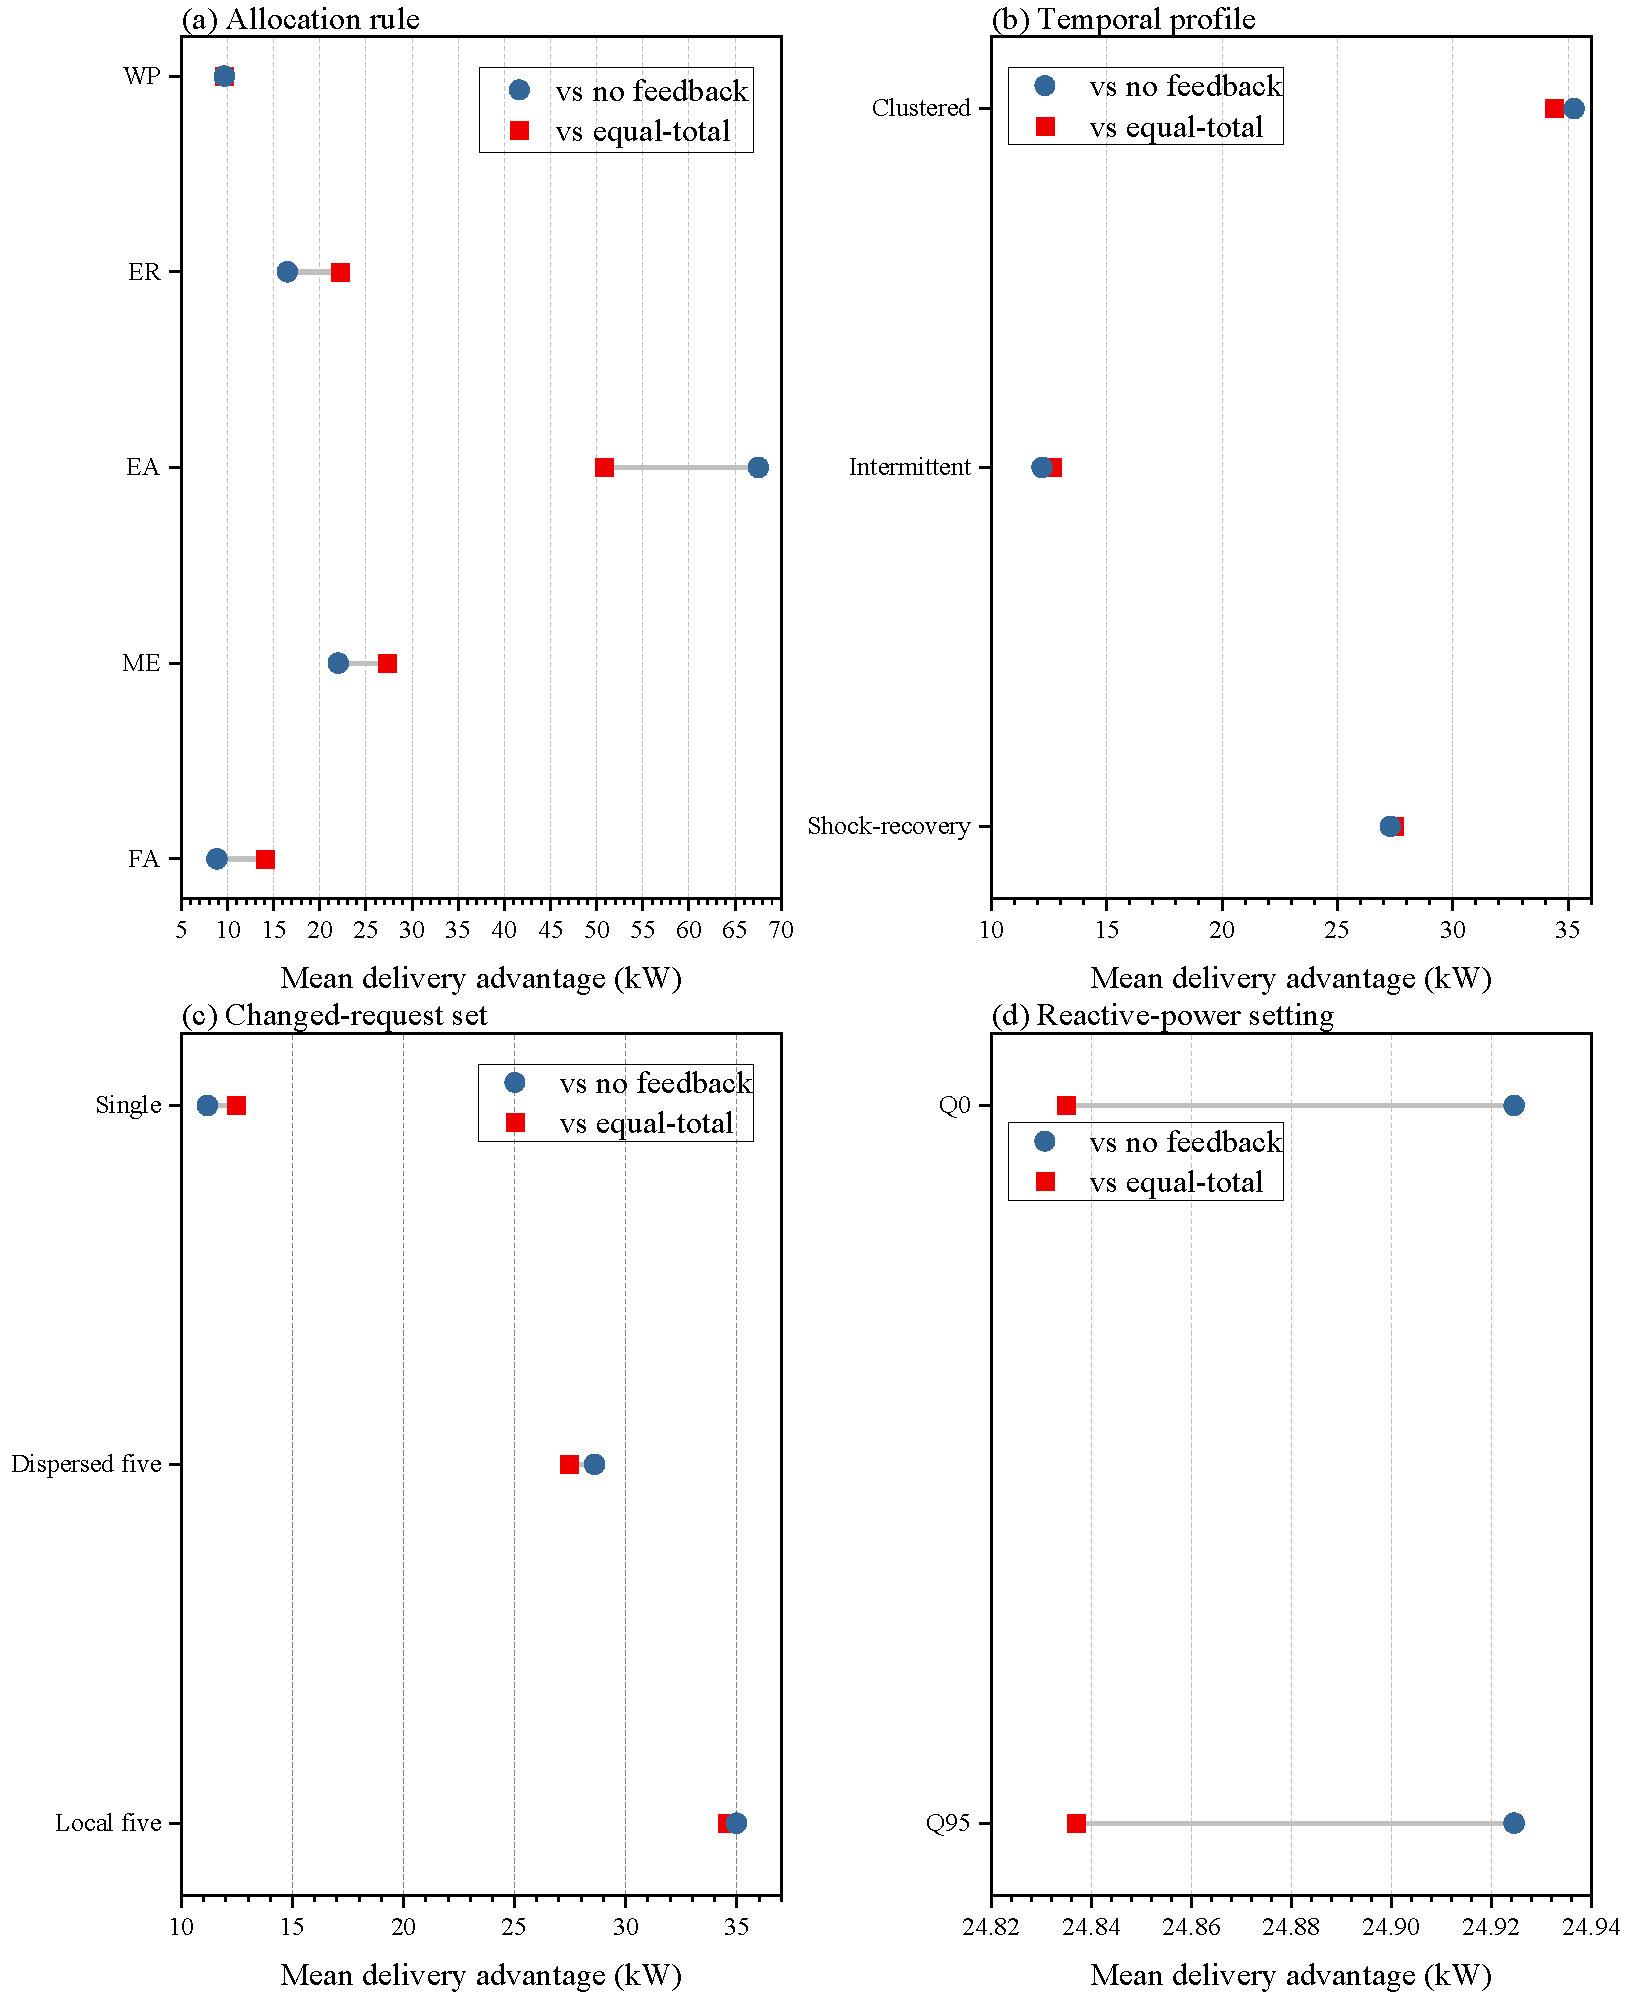
\includegraphics[width=\columnwidth]{figures/fig07_temporal_spatial_scaling.pdf}
\caption{Mean ECF delivery advantage at $\vartheta=0$ and
$\beta_{\mathrm{ECF}}=0.5$. Results are grouped by (a) allocation rule,
(b) temporal profile, (c) changed-request set, and (d) reactive-power setting. Blue circles
compare ECF with no feedback. Red squares compare ECF with the equal-total
control. WP, ER, EA, ME, and FA denote weighted proportional, equal reduction,
equal access, maximum export, and fairness-aware allocation, respectively. Q0
sets participant reactive power to zero, whereas Q95 uses 0.95-power-factor
absorption.}
\label{fig:temporal_spatial_scaling}
\end{figure}

\subsubsection{Feasible delivery gains do not imply equal access}

The delivery comparisons remain within the declared physical envelope. Both
sides of all 25,920 matched allocation comparisons pass nonlinear AC checks
for convergence, active- and reactive-power balance, voltage, and two-ended
branch apparent power. Since delivery can be below the award, we separately
check the resulting connection injections. All 22,520 distinct observed- and
replay-delivery states pass the same checks, with maximum branch utilization
of 90.91\% and no excess above the fixed synthetic ratings. Section S3.5 of
the \suppref{} gives the state counts and voltage extrema.
Fig.~\ref{fig:behavior_linked_physical_fairness}(a) shows the voltage margin:
the minimum bus-voltage magnitude minus the 0.95-per-unit (pu) lower limit.
Physical feasibility thus holds for both authorized and delivered export, including
cases where feedback reduces delivery.

More delivery does not automatically mean more equal access.
Fig.~\ref{fig:behavior_linked_physical_fairness} therefore reports both outcomes.
The Jain index measures capacity-normalized allocation equality, not broader
social fairness. At $\vartheta=0$, ECF yields a higher mean Jain-index change
than no feedback under all five rules, but most changes remain negative
relative to the forecast-based reference allocation. For EA, the change moves from $-2.4$ percentage
points without feedback to $0.1$ percentage points with ECF. The ECF values for
WP, ER, ME, and FA range approximately from $-0.8$
to $-0.5$ percentage points: ECF reduces the decline rather than producing
an absolute increase under these four rules. ECF also exceeds the equal-total control on
this mean metric for every rule. Panel (c) shows that mean delivery and
allocation-equality outcomes vary across rule--control combinations. Delivery
and allocation equality can therefore move in different directions. The
\suppref{} reports the corresponding unused-award, allocation-movement, and
total-authorization results.

\begin{figure}[!t]
\centering
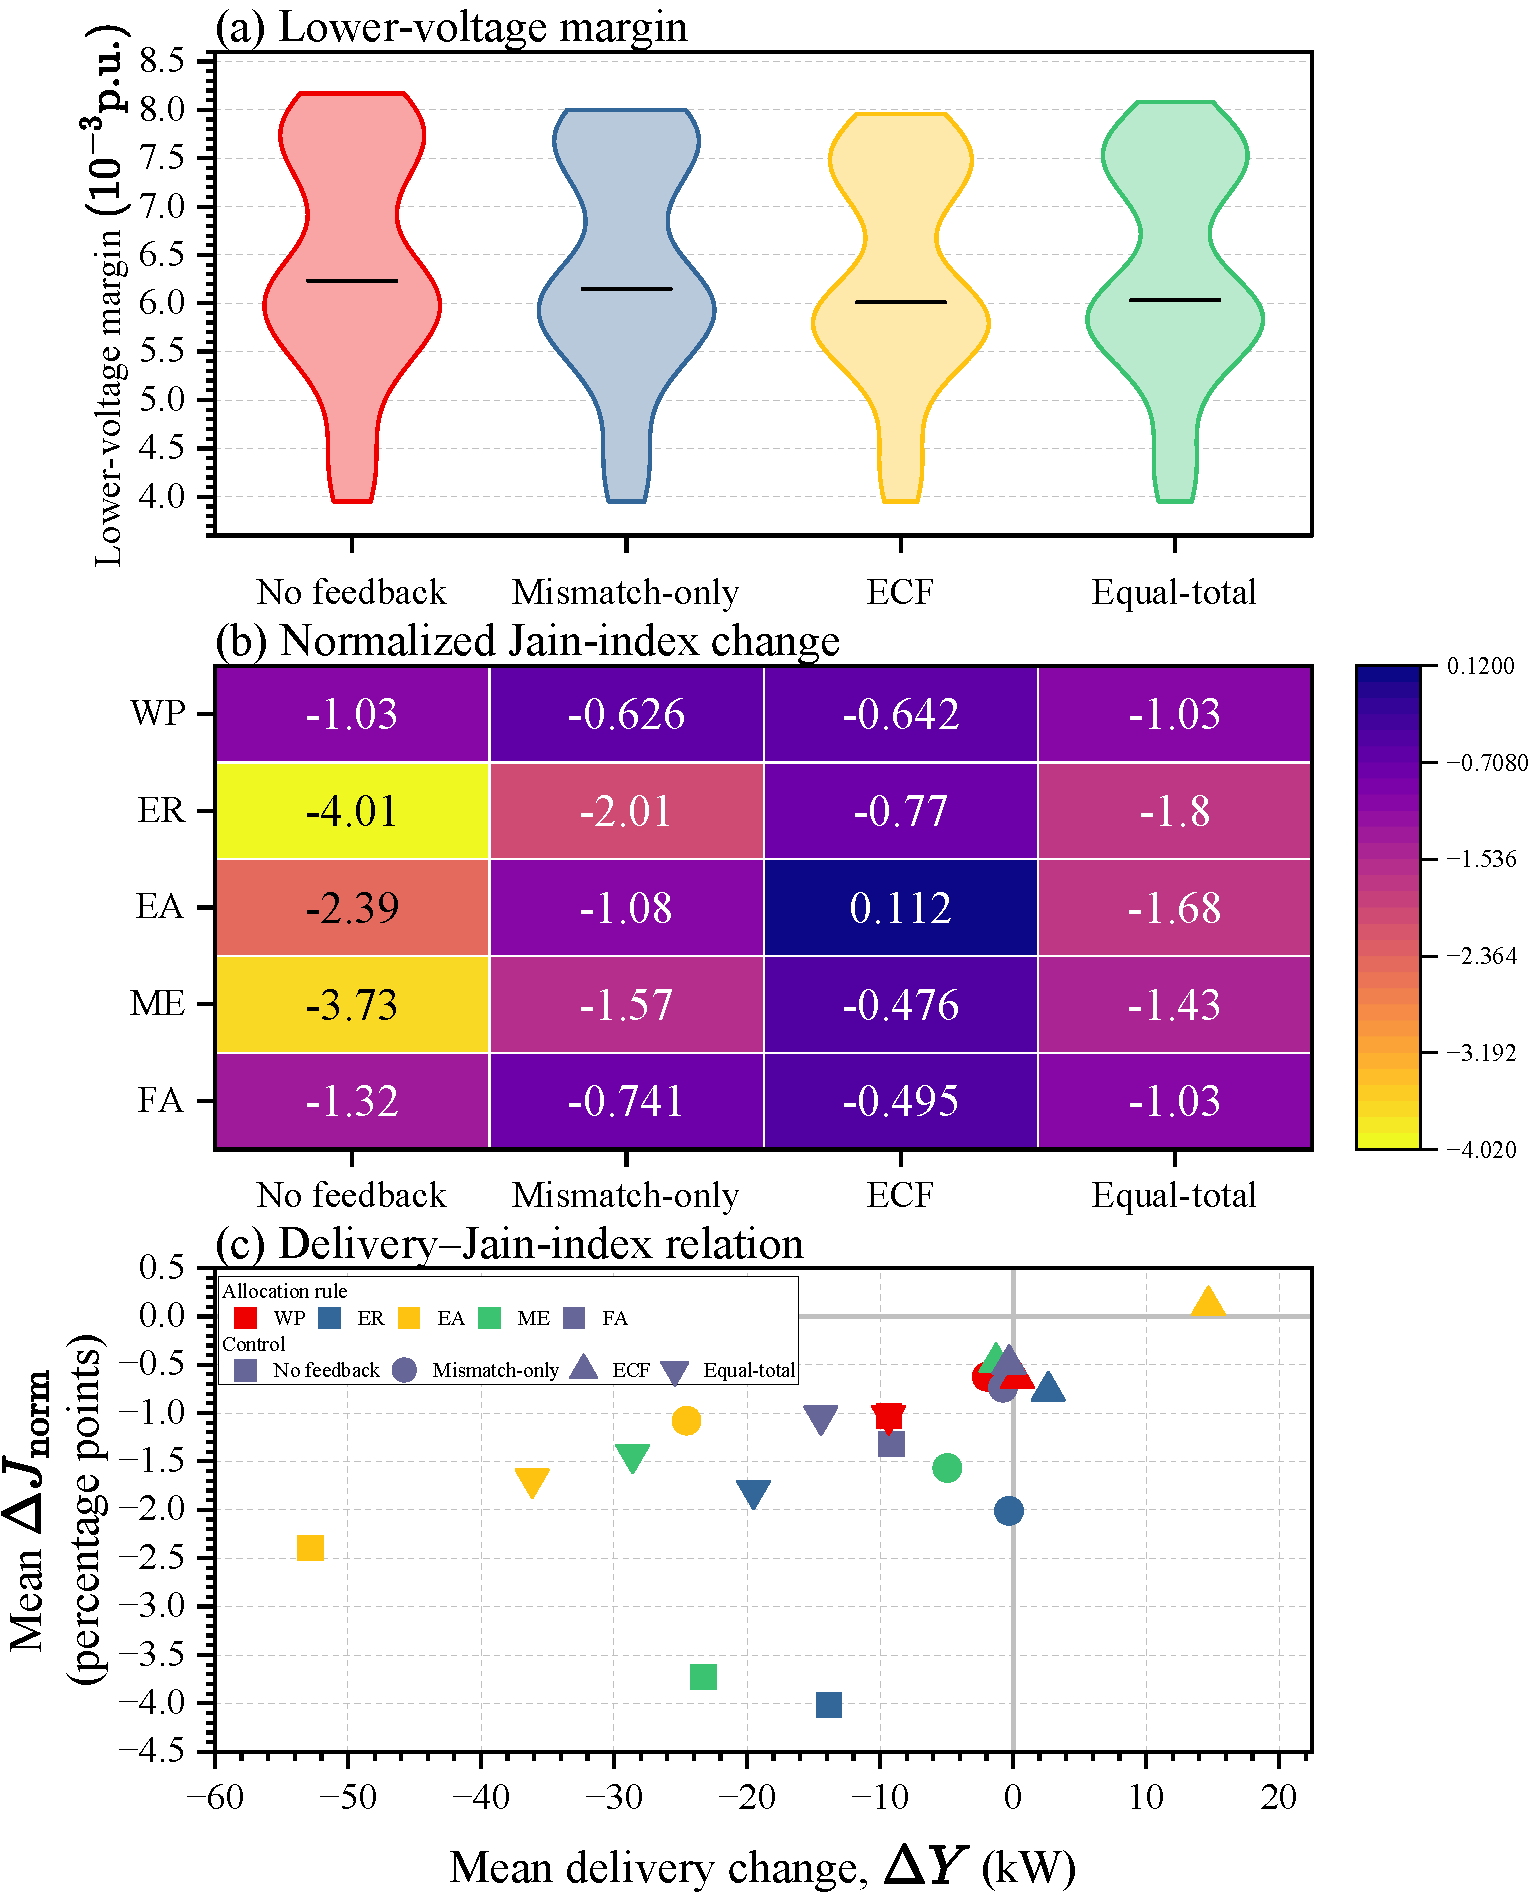
\includegraphics[width=\columnwidth]{figures/fig08_behavior_linked_ac_fairness.pdf}
\caption{Network-limit and allocation-equality outcomes for the AC-validated
controlled states. (a) Lower-voltage margin at $\vartheta=0$, where
the margin is the minimum bus-voltage magnitude minus the 0.95-pu lower limit.
Violin width shows empirical density, and the black segment
shows the median. (b) Mean change in the capacity-normalized Jain index, in
percentage points, relative to the forecast-based reference allocation, by
rule and control. Negative values indicate lower allocation equality than
that reference. (c) Mean total-delivery change plotted
against the corresponding Jain-index change. Colors identify allocation rules,
and marker shapes identify no feedback, mismatch-only feedback, ECF, and the
equal-total control. ECF and equal-total use $\beta_{\mathrm{ECF}}=0.5$.}
\label{fig:behavior_linked_physical_fairness}
\end{figure}

Thus physical feasibility, delivered electricity, and allocation equality
answer different questions. The observed gain in delivery is not a claim that
ECF maximizes every sharing objective. The \suppref{} reports secondary
allocation-formulation analyses under the same operating limits.

\subsection{Public-data replay gains delivery through a different allocation of access}
\label{sec:australian_results}

\subsubsection{Better use of access increases delivery, not just utilization}

ECF also outperforms equal-total reduction when requests and available output
follow public household profiles. Across 80 assessed network-days, it delivers
239.36~MWh of modeled export, 1.39~MWh (0.59\%) more than each of no feedback
and the equal-total control (Fig.~\ref{fig:australian_external_replay}).
The simulation combines a published Australian MV/LV network with measured
PV and load chronology. Available export and requests are constructed from
these profiles, rather than taken from linked operating records. Allocation
uses a common proportional scale, with daily ceiling initialization in the
primary comparison. Methods specifies the construction; the following
comparisons examine what changes the delivery gain.

More delivery here accompanies more authorization, rather than a smaller total
award. Relative to no feedback, authorization increases by 1.206~MWh and
unused authorization falls by 0.186~MWh. Together these changes account for
the 1.392-MWh delivery gain in
\eqref{eq:delivery_advantage_decomposition}. Selective request reduction
therefore improves delivery without requiring a reduction in total
authorization. Section S10 gives the complete energy balance, including the
almost identical contrast with the equal-total control.

Increased authorization is the larger term in this energy balance. Equal
admitted-request totals do not fix the total award: different request
distributions can admit different proportional allocation factors. Conversely,
uniformly scaling requests preserves their relative sizes. If the network
constraint still binds, the allocation factor can compensate for that scaling
and leave awards unchanged. The near-equality of no-feedback and equal-total
delivery is consistent with this property, derived in Section S4. Selective
updates change relative requests instead. The energy balance describes their
resulting delivery gain without assigning independent causal effects to
increased authorization and reduced unused awards.

The gain is uneven over time. ECF delivers more on 44 days, less on 32,
and the same amount on four against each control. Its mean daily gain is
17.4~kWh, with dependence-adjusted 95\% intervals of 5.1--29.7~kWh against
no feedback and 4.9--29.9~kWh against equal-total reduction. Only 483 of
3,840 half-hours (12.6\%) qualify for tightening. This frequency describes
how often the model finds a recoverable opportunity, not detection accuracy
or a guarantee of improvement on every day.

The connection-point gain also appears at the source terminal. Net source
exchange increases by 1.377~MWh against each control, retaining about 98.9\%
of the respective delivery gains. The feeder remains a net importer, so this
change means reduced upstream import. It includes the small increase in
circuit losses and changes in voltage-dependent passive-element exchange;
Section S10 separates those quantities. The delivery gain is therefore
visible at the feeder boundary, not only in the connection-level allocation totals.

Authorization utilization, $E_Y/E_X$, is 72.6\% under ECF and 72.4\%
under each of no feedback and the equal-total control. Here $E_Y$ and $E_X$
are delivered and authorized export energy over the assessed days.
Previous-day persistence gives a useful contrast: it omits the forecast
increment and uses 89.0\% of its authorization, yet delivers 50.33~MWh
less than ECF. A high utilization ratio alone can therefore conceal delivery
lost through an overly restrictive request. This contrast makes utilization
insufficient as an operating objective: withdrawing access can improve the
ratio even while reducing delivered energy.

All primary control trajectories satisfy the specified allocation and delivery
checks. Network limits nevertheless reduce the admitted-request scale in
44.4\% of ECF half-hours. The comparison therefore concerns how constrained
access is used, rather than a benefit obtained by allowing infeasible delivery.
Fig.~\ref{fig:australian_external_replay} reports the daily differences and
aggregate energy changes.

\begin{figure}[!t]
\centering
% Author-refined Origin export, 8 September 2026.
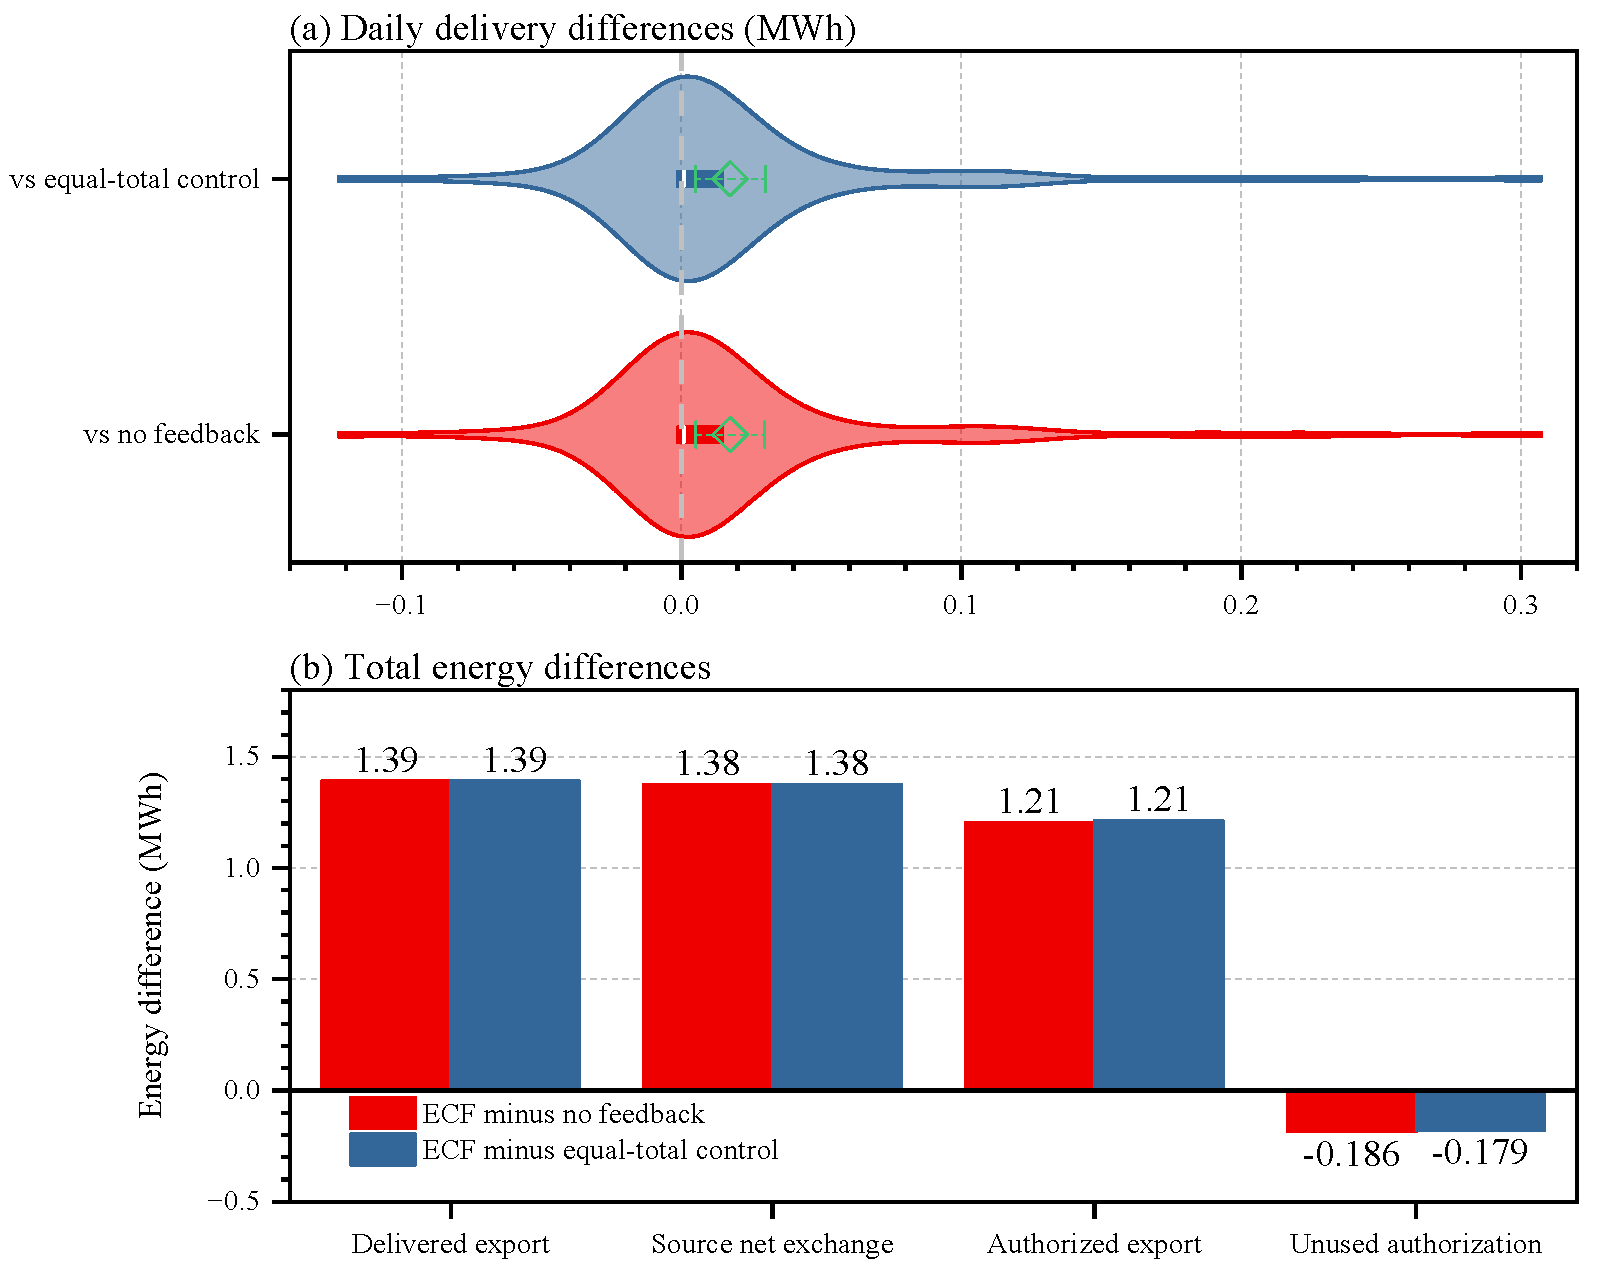
\includegraphics[width=\columnwidth]{figures/fig09_australian_external_replay.pdf}
\caption{Modeled delivery and authorization changes in the Australian
public-data replay. Available export is constructed from PV and load profiles.
(a) Paired daily delivery differences for ECF against no feedback and
the equal-total control. Violin width shows empirical density.
Dark boxes span the 25th--75th percentiles, and white ticks show medians. Green
diamonds show means; capped green lines show 95\% intervals adjusted for
short-range dependence between neighboring dates. (b) Aggregate 80-day
differences in delivered export, source-terminal net exchange, authorization,
and unused authorization. Each difference is ECF minus the indicated control.
Delivery equals authorization minus its unused portion. Here the delivery
gain accompanies increased authorization and reduced unused authorization.
Positive source-terminal differences indicate reduced net upstream import
over the assessed period.}
\label{fig:australian_external_replay}
\end{figure}

\subsubsection{Replay checks and update weight have distinct effects on delivery}
\label{sec:qualification_results}

A same-update comparison isolates the value of checking recoverable delivery.
Removing the replay test while keeping the update formula and gain unchanged reduces modeled
delivery from 239.36 to 232.93~MWh. ECF therefore delivers 6.42~MWh (2.76\%)
more, with higher delivery on 75 of 80 days. Its mean daily advantage is
80.3~kWh, with a dependence-adjusted 95\% interval of 69.3--91.2~kWh.

The control that skips these checks leaves 18.11~MWh less authorization unused,
but also grants 24.54~MWh less authorization. Reducing unused awards more
aggressively therefore sacrifices useful delivery. This comparison attributes
the difference to applying the replay criterion within the same recursive
update, rather than to a different smoothing formula. Both controls pass the
specified physical checks. Section S10.6 reports their energy totals,
participant-level differences, and the additional computation needed for replay.

Qualification determines whether to tighten the unused group's ceilings;
gain determines how strongly they respond. At $\beta_{\mathrm{ECF}}=0.25$, ECF
gains 1.34~MWh over each of no feedback and the equal-total control,
slightly less than at the primary gain of
0.5. At $\beta_{\mathrm{ECF}}=1$, it loses 3.04~MWh relative to no feedback
and 0.54~MWh relative to the equal-total control. The first mean-difference
interval is below zero; the second includes zero. Full replacement of the
ceiling by the latest target therefore offers no delivery advantage here.
Relative to no feedback, unit gain reduces total authorization by 14.55~MWh
and unused authorization by 11.51~MWh. Their difference explains the delivery
loss: some of the authorization removed would have been used.

After a qualifying replay, unit gain sets each unused-award participant's
next ceiling to its completed delivery. The largest net losses relative to
gain 0.5 occur at connections whose available output then rises while the new ceiling
still limits their request (Section S10 of the \suppref{}).
Together with the controlled gain sweep, this separates two requirements:
the completed-state comparison must be valid, and the later update must suit
the evolution of available export. Satisfying the first does not ensure the second.

The gain reversal persists when ceilings carry across midnight. In ten
consecutive-date blocks totaling 80 days, the longest spanning 35 days,
total delivery at each of the three gains differs from daily initialization
by less than 0.1~kWh. The primary advantage and the unit-gain loss are
therefore not explained by the daily reset. Section S10.8 relates ceiling
recovery to the update law and reports every block, including three in which
gain 0.5 delivers less than no feedback.

ECF also retains its aggregate delivery advantage when participants adjust
requests from their own past delivery. Each participant chooses among smaller
and larger requests, with preferences and ceilings carried across consecutive
days. Across the 80 dates and three random seeds, ECF delivers 1.44~MWh more
than no feedback and 4.53~MWh more than the same update without qualification;
both controls develop their own request histories. The equal-total shadow,
which follows ECF's history rather than learning independently, delivers
1.50~MWh less than ECF. These totals average the seeds within each date.
Compared with keeping request-choice probabilities fixed, preference updates
increase the advantage of retaining the replay checks, but do not establish a
larger advantage over no feedback. Section S10.15 reports the request model,
paired uncertainty, and daily variation. Thus ECF's mean benefit survives
experience-based request adjustment, without requiring requests to remain fixed.

\subsubsection{Record quality affects qualification and later delivery differently}
\label{sec:record_results}

The mean delivery gain tolerates several record perturbations, but this does
not establish that every replay remains correct. The four perturbations
scale the post-event record by $\pm10\%$, delay it by one interval, or
make a deterministic 10\% pattern of participant records unavailable and
substitute modeled delivery for those entries. Mean gains range from
16.4 to 18.0~kWh per network day against no feedback and from 16.3 to
18.0~kWh against the equal-total control. Every dependence-adjusted 95\%
interval remains above zero. The delivery comparison is therefore less
sensitive to these record changes than to the gain change. A separate
lower-bound calculation shows that individual completed-interval comparisons
have widely varying margins to record error (Section S10 of the \suppref).
Thus robustness of the mean gain does not imply equal robustness of each
replay decision.

Using a delivery lower bound protects the recovery test, but does not always
increase later delivery. A separate comparison runs both record treatments
at error radii of 1\%, 5\%, and 10\% of registered capacity, under common
overestimation and underestimation. Point-record control tightens after 11,
28, and 33 intervals in the three overestimation cases even though the
unperturbed model does not meet the recovery criteria. Lower-bound control
has no such interval in any of the six cases.

Underestimation creates the
opposite tradeoff: at the largest radius, lower-bound control misses 258 of
496 feasible recovery opportunities and delivers 269~kWh less than point-record
control. The mean daily difference is $-3.36$~kWh, with a 95\% interval of
$-6.39$ to $-0.34$~kWh. Across all six error cases, lower-bound control still
delivers 0.95--1.46~MWh more than no feedback, with positive mean-difference
intervals. All resulting allocation, delivery, and reference replay states
pass the specified physical checks. Section S10.9 of the \suppref{} gives
the complete comparisons. A reliable basis for an update and a beneficial
future response are thus separate requirements, even when the record error is bounded.

Fig.~\ref{fig:australian_sensitivity} collects the gain and record responses,
together with the complete-customer cohort. The latter broadens the calendar
to 361 days at the same load multiplier of 0.30. ECF gains 10.96~MWh over
each of no feedback and equal-total reduction, or 30.4~kWh per network day;
both mean-difference intervals remain above zero and all specified physical
checks pass. This result extends the positive comparison to a different
customer cohort and fuller calendar. It does not isolate record coverage,
because customer composition changes as well (Section S10).

\begin{figure}[!t]
\centering
% Author-refined Origin export, 8 September 2026.
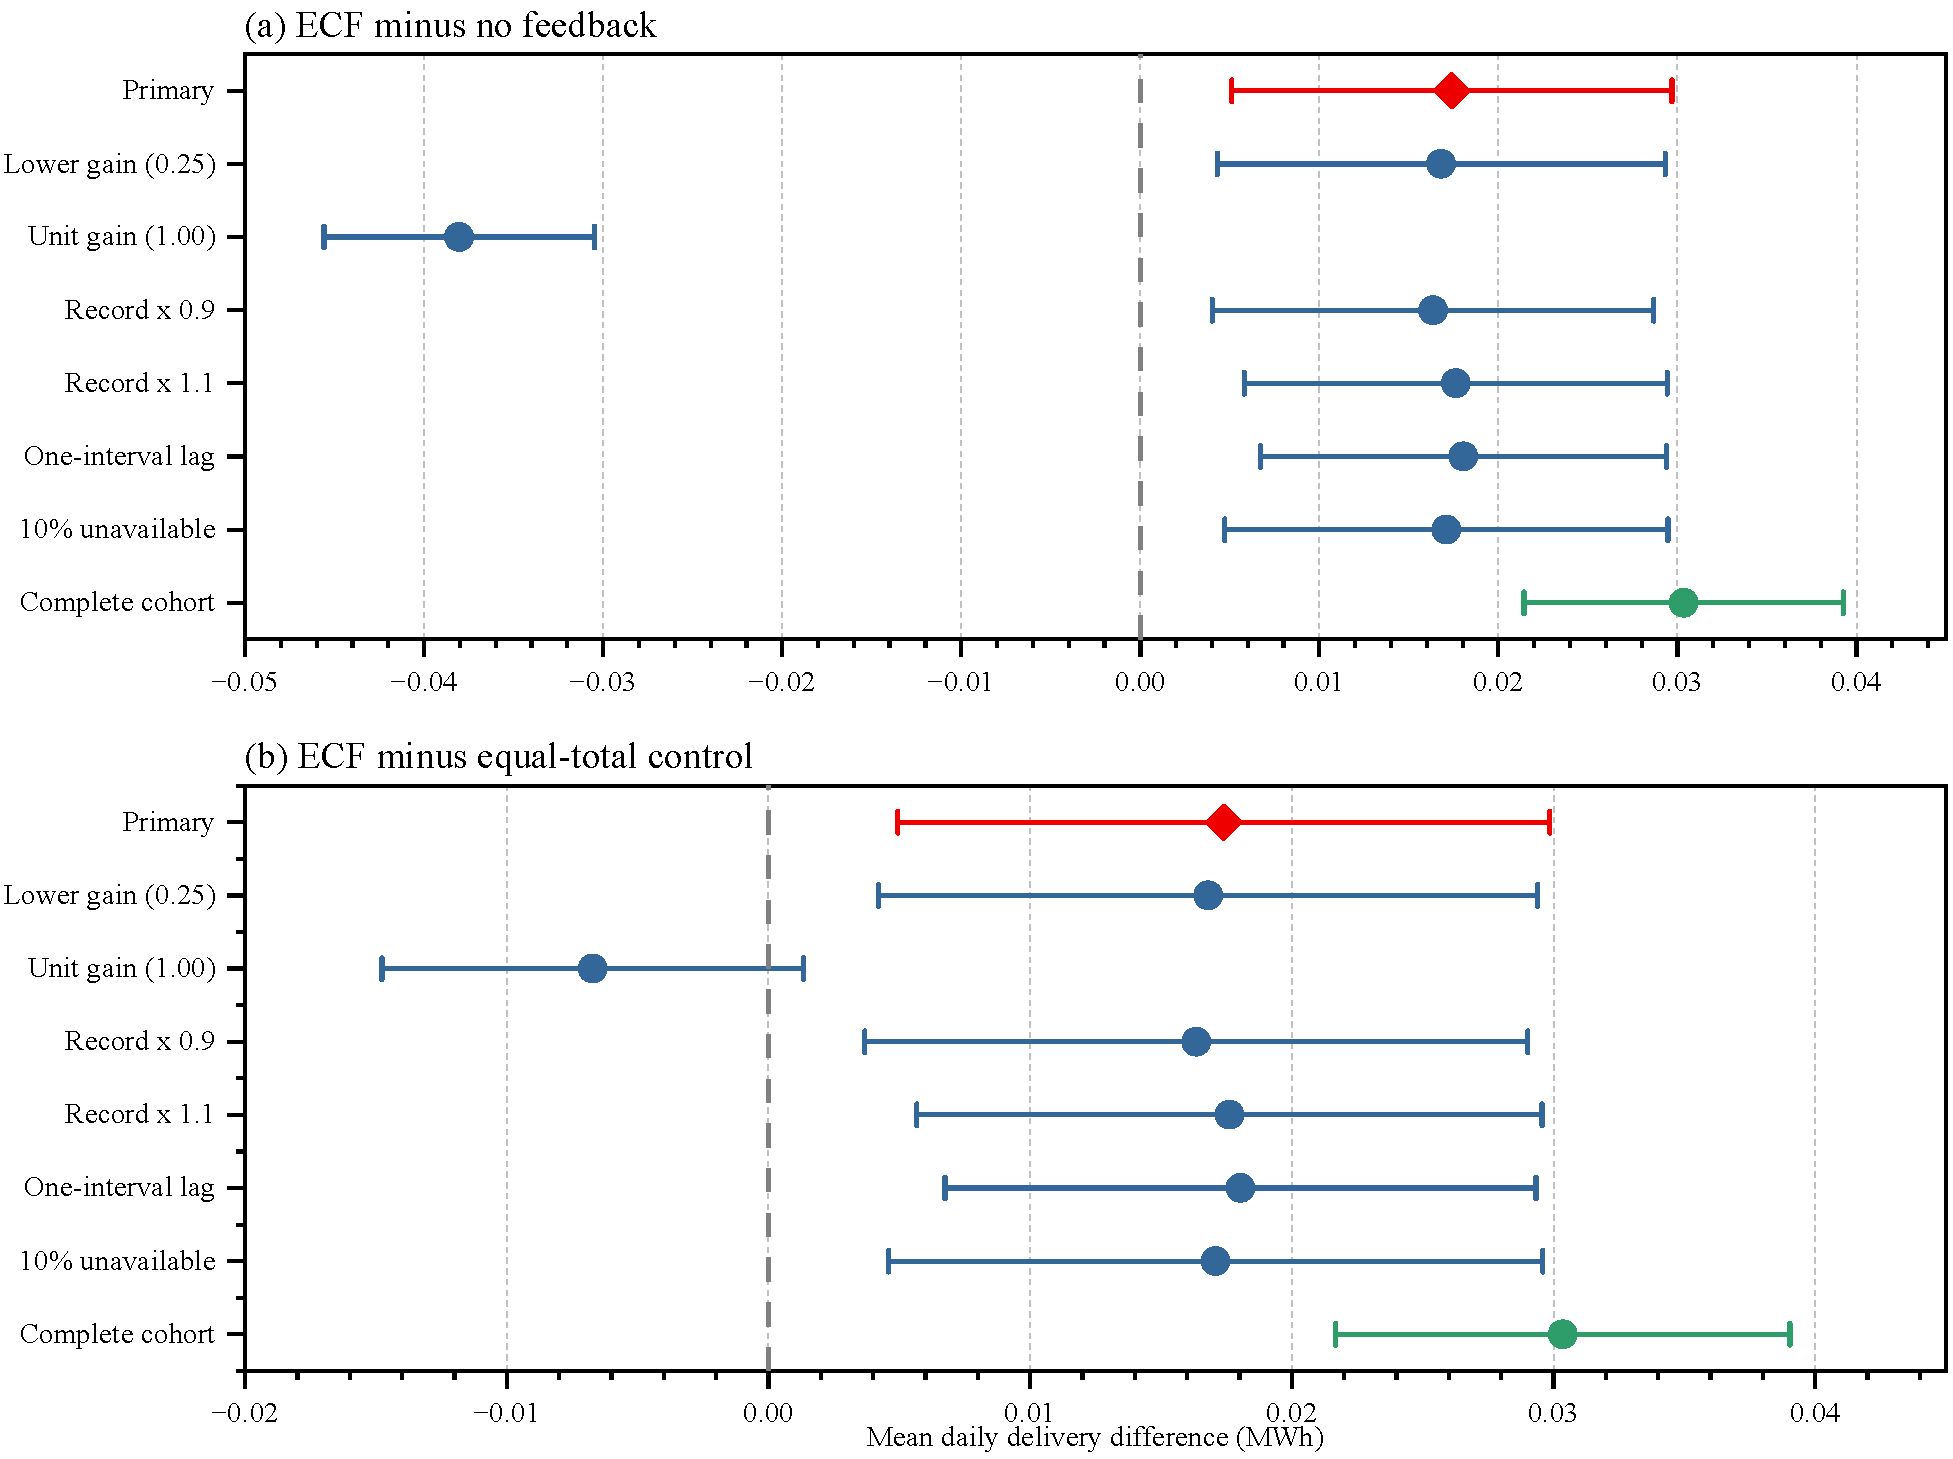
\includegraphics[width=\columnwidth]{figures/fig10_australian_sensitivity_forest.pdf}
\caption{Sensitivity of the Australian replay to feedback gain, post-event
record, and customer cohort. Markers show paired mean delivery differences per
network day. Bars show 95\% intervals adjusted for short-range dependence
between neighboring dates. (a) ECF minus no feedback. (b) ECF minus the
equal-total control. The red diamond denotes the primary unperturbed-proxy
result, and blue circles denote gain or record changes. Green markers denote
the complete-customer cohort, which uses the same load multiplier but changes
customer composition and calendar coverage. Every transformed available-export
record is floored at modeled delivery. All settings pass the specified
allocation and delivery checks; the zero line separates positive from
negative mean delivery differences.}
\label{fig:australian_sensitivity}
\end{figure}

\subsubsection{Spatial placement and available generation shape the benefit}
\label{sec:spatial_results}

The delivery advantage persists when the same household profiles occupy
different service connections. Across five alternative mappings, ECF gains
about 0.9--5.1~MWh over either no feedback or the equal-total control during
the same 80 days. All ten pointwise 95\% intervals for mean daily
differences are above zero. The positive aggregate comparison therefore
extends beyond the primary profile assignment, although its size varies
substantially with placement.

The smallest aggregate gain also illustrates why unused authorization alone
cannot measure success. In that mapping, ECF grants more authorization than
no feedback and leaves 0.35~MWh more unused, yet delivers 0.86~MWh more.
It gains delivery on 24 days and loses on 43, with no change on 13;
larger positive days outweigh the more frequent losses. Section S10.10 of
the \suppref{} gives each mapping's energy totals, daily differences, and
qualifying intervals. All allocation, delivery, and replay states pass the
specified physical checks.

The advantage also persists across PV capacities. At five levels spanning
half to one-and-a-half times the primary capacity, ECF gains 1.39--1.88~MWh
over either no feedback or the equal-total control during the same 80 dates.
Every pointwise mean-difference interval is above zero. The gain does not
increase monotonically with installed capacity, even though network limits
restrict requests more often. Relative to no feedback, delivery gained per
installed MW falls from 0.81 to 0.27~MWh across the smallest and largest
capacities. More PV therefore does not imply a proportionally larger benefit
from this feedback.

Capacity also changes the balance between authorization and its use. At half
the primary capacity, ECF grants 2.26~MWh more authorization and leaves
0.60~MWh more unused, yet delivers 1.66~MWh more than no feedback. At the
primary capacity, unused authorization instead decreases. Both responses
improve delivery, but only one reduces unused authorization.
Section S10.11 of the \suppref{} gives all four controls, daily comparisons,
and their satisfactory physical checks. Together, the placement and capacity
comparisons show why delivered energy is the relevant outcome: unused
authorization can rise or fall while delivery improves.

Changing the network section gives a related spatial comparison. ECF delivers
more than the equal-total control in all 13 published LV
sections. The 80-day differences range from 71.2 to 1,311.6~kWh.
Relative to no feedback, 12 sections gain delivery; LV26 loses 3.7~kWh.
All sections contain qualifying replay intervals. Selecting where requests
are reduced therefore improves on uniform reduction throughout this panel,
but it does not always improve on leaving requests unchanged.

All section trajectories satisfy the specified allocation and delivery checks.
Each section uses its own published model with the
primary chronology, profile mapping, load multiplier, authorization voltage
ceiling, and $\beta_{\mathrm{ECF}}=0.5$. These 13 sections belong to one
parent network collection. Their separate-model gains are not added to
estimate the coupled feeder's gain. The \suppref{} reports every section's
delivery difference, activation count, and physical-check status.

The representative-topology panel also contains null responses.
Six of the nine representative LV models contain qualifying replay intervals
and show positive aggregate delivery differences against both controls.
The models---G, J, L, M, N, O, P, Q, and R---come from the National
Low-Voltage Feeder Taxonomy Study \cite{geth2021lvtaxonomy}.
All four control trajectories pass the specified physical checks in every
model. J and Q have the largest gains: 543.0 and 960.5~kWh against no
feedback, and 611.7 and 982.1~kWh against the equal-total control.

G, M, P, and R also have positive differences, although M qualifies only
twice and gains just 0.1~kWh over no feedback. L, N, and O have no
qualifying intervals and remain unchanged. The common feedback setting
therefore produces substantially different responses across the published
structures. These results extend the positive comparison beyond one topology
while identifying models where no update is warranted by the replay.
Methods gives the electrical inclusion criteria.
Fig.~\ref{fig:taxonomy_panel} and the \suppref{} report each model separately.

Spatially uneven gains also appear within the primary feeder. Of its 418
participants, 330 deliver more over the 80 days than without feedback and
88 deliver less; the largest individual loss is 7.3~kWh. Section S10.14
reports the cumulative and daily distributions. A positive feeder total
therefore does not imply that every connection benefits, just as a favorable
mean across days does not imply improvement on every day.

\begin{figure}[!t]
\centering
% Author-refined Origin export, 8 September 2026.
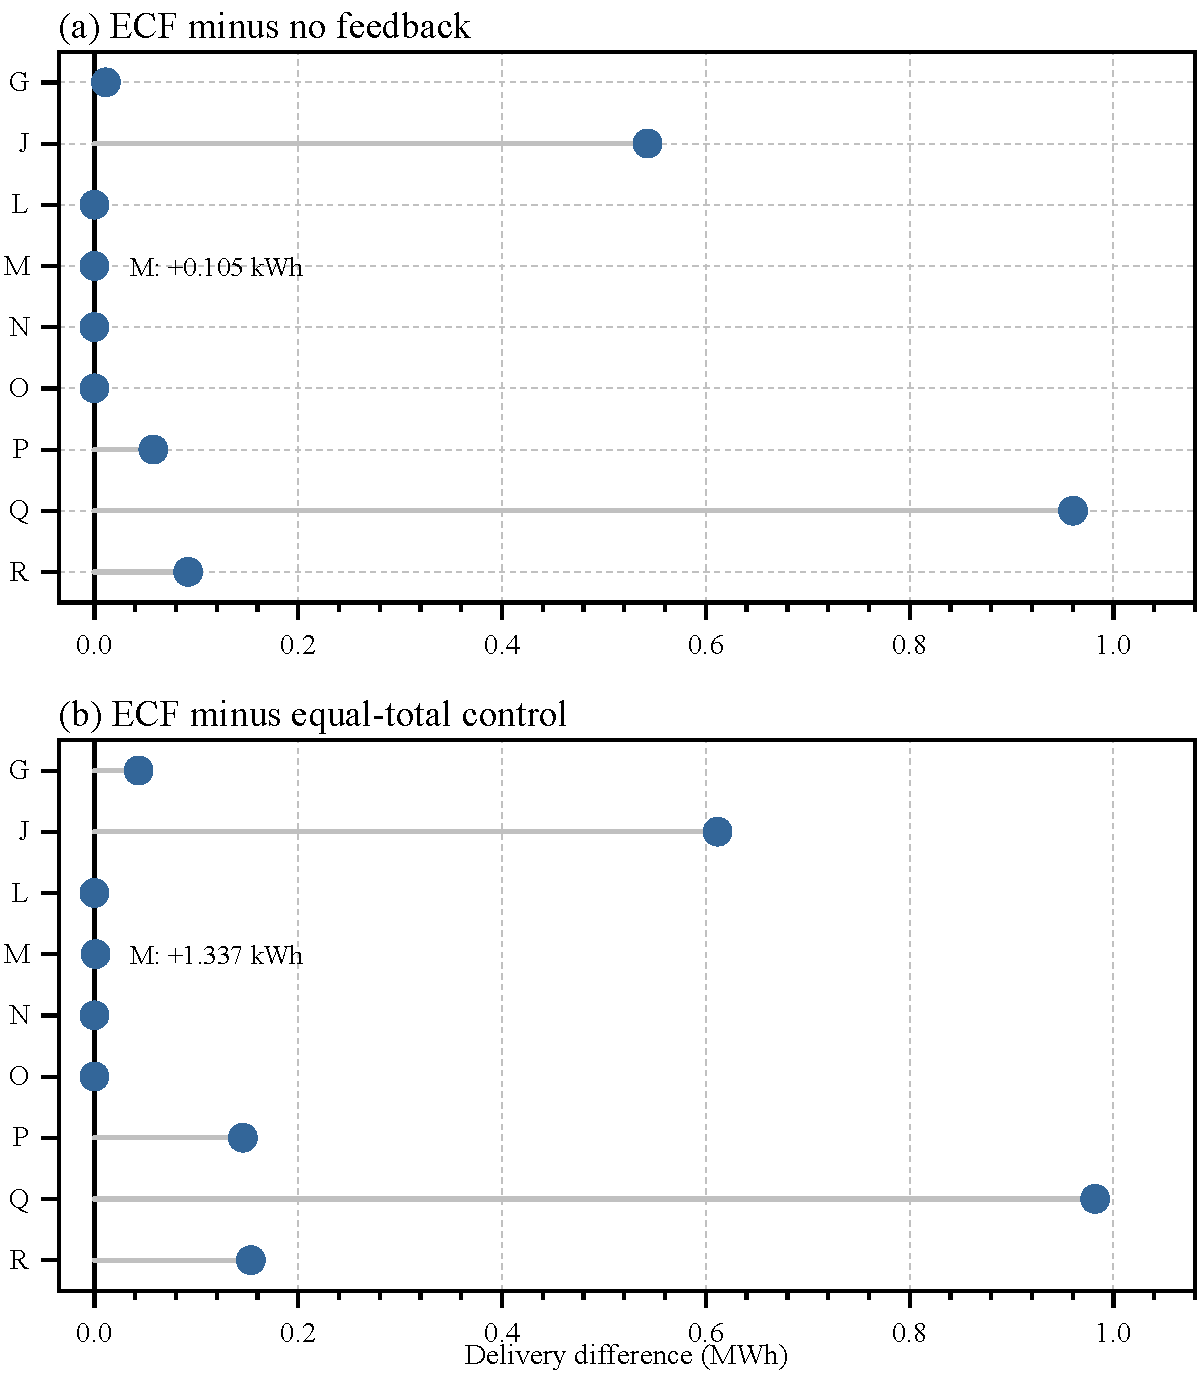
\includegraphics[width=\columnwidth]{figures/fig11_public_lv_taxonomy_panel.pdf}
\caption{Delivery differences across nine published representative low-voltage
models. Each marker is the 80-day ECF-minus-control total for one model;
horizontal stems connect zero to that total.
(a) ECF minus no feedback. (b) ECF minus the equal-total control.
All models pass the specified voltage and transformer checks across the four
controls. Six models have positive totals; L, N, and O have no qualifying
interval and zero difference. Qualifying-interval counts are reported
separately in the SI. Results are not pooled across models.}
\label{fig:taxonomy_panel}
\end{figure}

\subsection{Implications for the use of constrained export access}
\label{sec:discussion}
\label{sec:policy_implications}

The findings suggest that export-access arrangements should be evaluated by
the electricity delivered as well as the permission allocated. Persistence
uses a larger fraction of its award but delivers substantially less electricity.
The same update without replay qualification removes more unused authorization
than ECF, yet also delivers less. Neither minimizing unused awards nor
maximizing authorization utilization is therefore a sufficient operating objective.
A useful adjustment must preserve access that can be used when output recovers.

\paragraph{Use completed records to complement allocation and settlement.}
Network-aware allocation already accounts for electrical location. The
equal-total comparison shows why later request adjustments also need to
consider where available electricity remains: an identical aggregate request
reduction can produce different awards and delivery. Completed records provide
a way to test that opportunity while retaining the chosen sharing rule.
This is a distinct role from shortfall settlement, which changes the incentive
to request access. The state-dependent relationship in
Fig.~\ref{fig:endogenous_request_choice}(d) explains why one shortfall cost
cannot represent every loss of delivery elsewhere.

Flexible export arrangements provide a relevant setting for this use of
operating information
\cite{sapn2024dapr,cpuc2022e5230,eu2024flexibleconnections}.
The proposed addition is a basis for updating requests, not a replacement
for network limits or a new financial settlement. Source-terminal accounting
shows that the resulting connection-level gain can also reduce upstream
import after network losses and passive-element exchange are included.
This connects the allocation decision to feeder energy exchange.

\paragraph{Separate the reason to tighten from the speed of response.}
A favorable replay identifies a missed opportunity in the completed interval.
It does not determine how much access the same participants will need next.
The gain reversals, recovery trajectories, and cross-day comparison show why
these are different questions. A large response to low completed delivery can
restrict export when available output rises. Gain selection should therefore
use subsequent delivered energy and ceiling recovery, rather than the
frequency of qualifying replays. Evaluation against both no feedback and
equal-total reduction is important: the LV26 comparison improves on uniform
reduction but not on leaving requests unchanged.

\paragraph{Track who gains and who loses.}
The spatial comparisons show variation in both aggregate benefit and its
distribution. The primary feeder gains delivery overall, but some participants
lose cumulative delivery. Operational assessment should therefore retain
participant-level delivery and the duration of restrictive ceilings alongside
the feeder total. Replay qualifies the unused-award group collectively;
it does not identify each member's causal contribution. Its output supports
an operational update, not individual blame or a charge for displaced energy.

\paragraph{Match the information requirement to the intended use.}
A pilot needs linked requests, awards, metered delivery, and available-export
records, with connection identities and the applicable network model.
It need not reveal participants' private forecast distributions. However,
available export must remain valid for the alternative allocation; responses
of storage, demand, or local controllers must be modeled when access changes
them. Independently validated error bounds can make the recovery comparison
conservative, while AC feasibility is checked separately. When increased
replay delivery cannot be established, ECF lets ceilings recover toward
registered capacity. The bounded-record results also show the cost of caution:
rejecting more doubtful updates can forgo later delivery gains. Record
validation, communication, and replay computation must therefore be assessed
against the additional energy delivered, rather than inferred from the
activation rate.

\paragraph{Scope and next evidence.}
The controlled study connects request incentives to delivery under five rules
within a declared synthetic medium-voltage envelope. The public simulations
add measured household chronology, customer-voltage limits, and native
transformer ratings, but construct the profile mapping, requests, and
available-export record. Spatial and capacity comparisons vary these
conditions without estimating the prevalence of opportunities across feeders.
The primary calendar covers 80 seasonally incomplete days; continuous memory
is tested within observed date blocks of up to 35 days. Experience-based
request adjustment is included, whereas anticipation of future ceilings and
strategic manipulation of availability records are not. Linked field records
and longer operating histories would test those behaviors and the cost of
implementation. Annual energy, market value, household welfare, generation
displacement, and emissions require their own calendar coverage and models.
The SI reports the physical-check coverage separately from these inference
limits: a feasible trajectory can still have an unfavorable delivery outcome.

\FloatBarrier

\section{Methods}
\label{sec:methods}

\EESsystemmethod
\EESbehaviormethod
\EESallocationmethod
\EESfeedbackmethod
\EESphysicalmethod
\EESexperimentalmethod
\EESaustralianmethod

\section{Conclusions}
\label{sec:conclusion}

An unused export award does not, by itself, establish that another participant
could have delivered more electricity. Larger requests can also protect useful
delivery when output is uncertain. ECF therefore tests whether an alternative
allocation of a completed interval would have enabled more delivery elsewhere
and in total before adjusting later request ceilings.

The results show that reducing the same total request can produce different
delivery outcomes depending on whose requests are reduced. Network location
and available output determine whether released access can be used. Less
unused authorization is not, by itself, a sufficient measure of improvement.
Selective updates can increase delivered electricity by changing the
distribution of access, without requiring a reduction in total authorization.

Finding that others could have delivered more in a completed interval does
not determine how strongly future access should change. An update that follows the latest
shortfall too closely can restrict export when output recovers. Effective
feedback must therefore combine a justified reason to adjust requests with an
update that preserves access for later recovery.

Completed operating records can thus support better use of existing export
capacity while retaining the network limits, allocation rule and settlement
arrangements. The objective is to deliver more available electricity, rather
than minimize unused permission. Field evaluation should validate the
available-export records and examine how participants alter requests when they
anticipate future ceiling adjustments.

\section*{Author contributions}
Junjie Huang: conceptualization, methodology, software, formal analysis,
investigation, visualization, data curation, and writing---original draft.
Tao Yu and Yusheng Xue: conceptualization, supervision, funding acquisition, and
writing---review and editing. Zhenning Pan, Yufeng Wu, and Wencong Xiao:
methodology, validation, and writing---review and editing. Rankai Zhu:
validation, data curation, and writing---review and editing. Jie Huang:
validation and writing---review and editing.

\section*{Conflicts of interest}
There are no conflicts to declare.

\section*{Data availability}
The SI, simulation and analysis code, calculated result tables, figure data,
and computational environment specification are deposited in the project
repository\textsuperscript{\dag}. The repository is currently private for author
review; access for editors and reviewers will be arranged before submission.
The cited 141-bus case, CSIRO/GridQube network collection (DOI
10.25919/ghnz-bk28), and Ausgrid Solar Home Electricity Data are obtained from
their original distributors under the applicable terms. The repository provides
source identifiers, preprocessing code, parameter files, date selections,
mapping tables, file hashes, and reproduction instructions. It distinguishes
checks of saved results from full simulation reruns and identifies the
external inputs and auxiliary caches needed for the latter.

\section*{Acknowledgements}
This work was funded by State Grid Electric Power Research Institute
Co., Ltd., Project ``Interaction and Coordination Technology of
Cyber-Physical-Social Elements (II)'' (SGNR0000KJJS2505736).

\vfuzz=2pt
\begingroup
\setstretch{1.0}
\setlength{\bibsep}{0pt}
% Start column balancing on the final reference page, not at the start of the list.
% Recheck this anchor if preceding text changes pagination.
\let\ECForiginalbibitem\bibitem
\renewcommand{\bibitem}[2][]{%
  \def\ECFcurrentkey{#2}\def\ECFbalancekey{mallaki2021strategic}%
  \ifx\ECFcurrentkey\ECFbalancekey\balance\fi
  \ECForiginalbibitem[#1]{#2}}
\bibliographystyle{rsc}
\bibliography{references}
\endgroup

\end{document}
